%
% Honours Thesis template that uses the memoir package
%
\documentclass[a4paper,12pt]{memoir}


\usepackage{amsmath,amssymb,amsthm}
\usepackage{graphicx,color,xcolor}
\usepackage{thmtools}
\usepackage[linktocpage=true]{hyperref}


\usepackage{tikz}
\usetikzlibrary{calc,backgrounds}
\usepackage{amsmath}
\usepackage{amssymb}
\usepackage{float}
\usepackage{graphicx}
\usepackage{svg}
\usepackage{pgfplots}
\usepackage{xcolor}
\usepackage{subcaption}

\setcounter{MaxMatrixCols}{20} % Increase max allowed columns

\usetikzlibrary{fadings}
\tikzfading
  [name=fadeLR,
   left color=transparent!100,  % fully transparent at the left
   right color=transparent!0]   % fully opaque at the right
\tikzfading
   [name=fadeRL,
    right color=transparent!100,  % fully transparent at the left
    left color=transparent!0]   % fully opaque at the right

\definecolor{pale_yellow}{HTML}{ffef96}

\definecolor{col1}{HTML}{7570B3}
\definecolor{col2}{HTML}{D95F02}
\definecolor{col3}{HTML}{1B9E77}
\definecolor{col4}{HTML}{E7298A}
\definecolor{col5}{HTML}{66A61E}
\definecolor{col6}{HTML}{E6AB02}

\definecolor{col1_light}{HTML}{8f8ac0}
\definecolor{col2_light}{HTML}{d88a5f}
\definecolor{col3_light}{HTML}{6fb89f}
\definecolor{col4_light}{HTML}{e08fb5}
\definecolor{col5_light}{HTML}{8fb87f}
\definecolor{col6_light}{HTML}{e0c15a}



\hypersetup{
    colorlinks,
    linkcolor={blue!90!black},
    citecolor={blue!90!black},
    urlcolor={blue!90!black}
}

\newtheorem{theorem}{Theorem}[section] 
\newtheorem{lemma}[theorem]{Lemma}    
\newtheorem{propn}[theorem]{Proposition}    
\newtheorem{corollary}[theorem]{Corollary}    
\newtheorem{example}[theorem]{Example}    
\newtheorem{question}[theorem]{Question}    
\newtheorem{exercise}[theorem]{Exercise}    
\newtheorem{conjecture}[theorem]{Conjecture}
\newtheorem{definition}[theorem]{Definition}
\newtheorem{property}[theorem]{Property}
\newtheorem{claim}{Claim}
\newtheorem{fact}{Fact}
\newtheorem{remark}[theorem]{Remark}
\newtheorem{problem}[theorem]{Problem}


\declaretheoremstyle[
  headfont=\normalfont\bfseries,
  numbered=unless unique,
  bodyfont=\normalfont,
  spaceabove=1em plus 0.75em minus 0.25em,
  spacebelow=1em plus 0.75em minus 0.25em,
  qed=$\bullet$,
]{exmpstyle2}

\declaretheorem[
  style=exmpstyle2,
  title=Example,
  refname={example,examples},
  Refname={Example,Examples}
]{example2}

\renewcommand{\le}{\leqslant}
\renewcommand{\ge}{\geqslant}
\renewcommand{\leq}{\leqslant}
\renewcommand{\geq}{\geqslant}

% \setlrmarginsandblock{4cm}{2cm}{*}
\setlrmarginsandblock{3cm}{3cm}{*}
\setulmarginsandblock{3.5cm}{3cm}{*}
\checkandfixthelayout

\chapterstyle{ger}   % you can easily change the chapter style here
\nouppercaseheads
\tightlists

\graphicspath{ {Images/} }

\makeindex

\begin{document}

\begin{titlingpage}

\vspace*{0.4cm}
\begin{center}
{ \huge \bfseries Feature Selection of Ordinal Partitions for Echo State Networks  \\[0.4cm] }
\vspace{1cm}
\end{center}
\begin{center}
\large
by\\
\vspace{1.5cm}
\textbf{Hector Morlet}\\
BSc\\
\vspace{1cm}
\end{center}
\vspace{3cm}

\begin{tabular}{ p{2.2cm}l } 
Supervisors: & Professor Michael Small\\
			&  Doctor Eugene Tan
\end{tabular}

\vfill
\begin{center}
This thesis is presented for the partial requirements of the degree of\\ Bachelor of Science with honours
of the University of Western Australia.\\
\today
\end{center}
\vspace{2.5cm}
\end{titlingpage}

\frontmatter
\chapter*{Abstract}
\addcontentsline{toc}{chapter}{Abstract}

This thesis will present research into the use of the ordinal partitioning of time series data to inform the creation of an Echo State Network to predict this data.
\chapter*{Acknowledgements}
\addcontentsline{toc}{chapter}{Acknowledgements}

This thesis is the result of the many patient meetings and helpful guidance provided by Eugene and Michael, and I am very grateful for their support.

\tableofcontents
\newpage
\listoffigures 
\newpage
\listoftables

\mainmatter
% !TEX root = ../HonoursThesisTemplate.tex

\chapter{Chapter title}

In David Hilbert's\index{Hilbert, David} paper \cite{Hilbert:1901aa}, it was shown that \dots

\begin{theorem}
All roads lead to Rome.
\end{theorem}
% !TEX root = ../HonoursThesisTemplate.tex

\chapter{Ordinal Partitions}

    
`Ordinal analysis', first introduced by Bandt and Pompe (2002), proposed using the ordering of data points to partition a time series. Each data point in the timeseries is partitioned according to the ordering of its preceding points, and assigned a unique `ordinal symbol', for example numbers from 1 to 6.

The probabilities of the timeseries transitioning from one partition to another can be calculated, giving the `ordinal transition probabilities'.

\begin{figure}
    \centering
    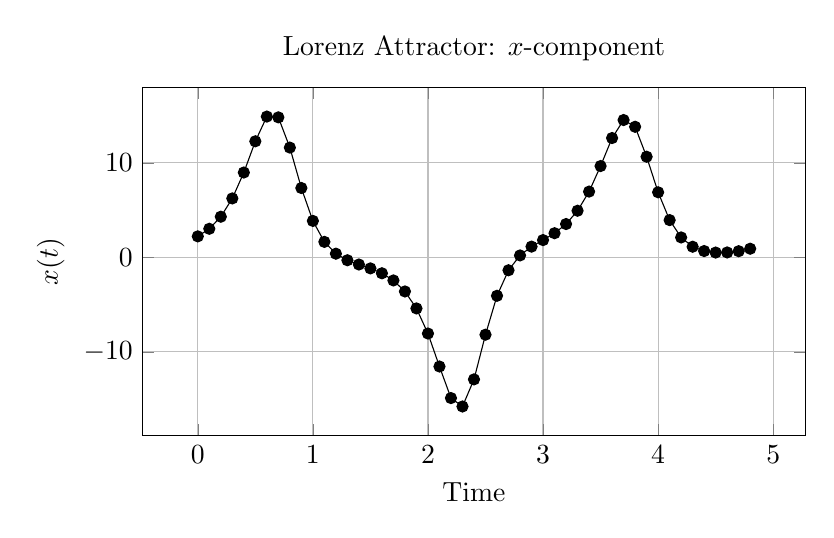
\begin{tikzpicture}
        \begin{axis}[
            xlabel={Time},
            ylabel={$x(t)$},
            title={Lorenz Attractor: $x$-component},
            width=10cm, height=6cm,
            grid=major
        ]
        % Data generated by solving dx/dt = sigma(y - x), etc. in Python
        \addplot[black, mark=*, mark options={black}] coordinates {
            (0.0, 2.2165566502619796)
            (0.1, 3.0181360987381685)
            (0.2, 4.2948078524935065)
            (0.3, 6.231121537780632)
            (0.4, 8.970926893912857)
            (0.5, 12.272230400810887)
            (0.6, 14.887997312478161)
            (0.7, 14.803117347063516)
            (0.8, 11.606868473299526)
            (0.9, 7.330990437181266)
            (1.0, 3.85191889651296)
            (1.1, 1.6347534154776406)
            (1.2, 0.3853895148599277)
            (1.3, -0.30838099414996695)
            (1.4, -0.7586726217449103)
            (1.5, -1.1695821908357407)
            (1.6, -1.6858338981790886)
            (1.7, -2.443141458426554)
            (1.8, -3.6086854451117074)
            (1.9, -5.40339197322587)
            (2.0, -8.058505977971057)
            (2.1, -11.547145254692042)
            (2.2, -14.884182443761347)
            (2.3, -15.775516623377253)
            (2.4, -12.908181797239536)
            (2.5, -8.181376578133673)
            (2.6, -4.06724026097539)
            (2.7, -1.3665393788429014)
            (2.8, 0.20110496364168012)
            (2.9, 1.1324784341364973)
            (3.0, 1.8245674314417792)
            (3.1, 2.5516132966355554)
            (3.2, 3.5214281335608555)
            (3.3, 4.926987945369609)
            (3.4, 6.951562500713474)
            (3.5, 9.654345729238477)
            (3.6, 12.617195234374243)
            (3.7, 14.521825487882024)
            (3.8, 13.806356286601272)
            (3.9, 10.64113968132102)
            (4.0, 6.880279139891668)
            (4.1, 3.9367704788159394)
            (4.2, 2.1029851064946445)
            (4.3, 1.121305395878461)
            (4.4, 0.665491176850325)
            (4.5, 0.5051437108082056)
            (4.6, 0.5156168027361644)
            (4.7, 0.6490783162490397)
            (4.8, 0.9105168761220792)
        };
        \end{axis}
    \end{tikzpicture}
    \caption{This is the caption}
    \label{fig:label}
\end{figure}

\begin{figure}
    \begin{center}
        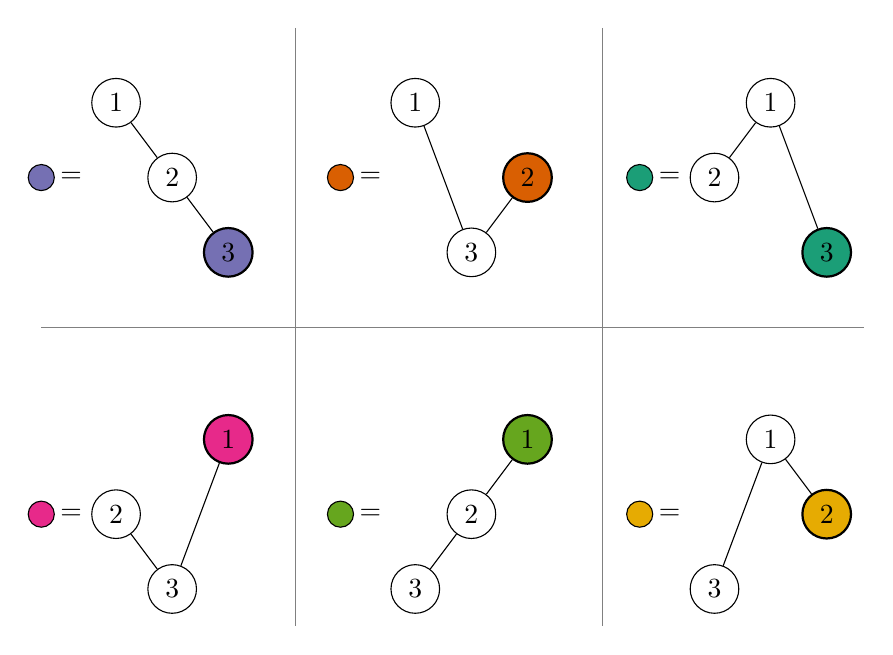
\begin{tikzpicture}[scale=0.95]
            % partition 1

            \node[circle, draw, fill=col1] (topleft) at (-5.0, 3) {};

            % Draw the equality sign
            \node at (-4.6, 3) {$=$};
            
            % Draw the nodes in the lower part
            \node[circle, draw] (1_2) at (-4.0, 4) {1};
            \node[circle, draw] (1_1) at (-3.25, 3) {2};
            \node[circle, draw, thick, fill=col1] (1_3) at (-2.5, 2) {3};
            
            % Draw edges
            \draw (1_1) -- (1_2);
            \draw (1_1) -- (1_3);

            % Draw dividing line
            \draw[gray, very thin] (-1.6, 5) -- (-1.6, -3);

            % partition 2

            \node[circle, draw, fill=col2] (topcentre) at (-1, 3) {};

            % Draw the equality sign
            \node at (-0.6, 3) {$=$};
            
            % Draw the nodes in the lower part
            \node[circle, draw] (2_2) at (0, 4) {1};
            \node[circle, draw] (2_1) at (0.75, 2) {3};
            \node[circle, draw, thick, fill=col2] (2_3) at (1.5, 3) {2};
            
            % Draw edges
            \draw (2_1) -- (2_2);
            \draw (2_1) -- (2_3);

            % Draw dividing line
            \draw[gray, very thin] (2.5, 5) -- (2.5, -3);

            % partition 3

            \node[circle, draw, fill=col3] (topleft) at (3.0, 3) {};

            % Draw the equality sign
            \node at (3.4, 3) {$=$};
            
            % Draw the nodes in the lower part
            \node[circle, draw] (3_2) at (4.0, 3) {2};
            \node[circle, draw] (3_1) at (4.75, 4) {1};
            \node[circle, draw, thick, fill=col3] (3_3) at (5.5, 2) {3};
            
            % Draw edges
            \draw (3_1) -- (3_2);
            \draw (3_1) -- (3_3);

            % Draw dividing line
            \draw[gray, very thin] (-5, 1) -- (6, 1);

            % partition 4

            \node[circle, draw, fill=col4] (bottomleft) at (-5.0, -1.5) {};

            % Draw the equality sign
            \node at (-4.6, -1.5) {$=$};
            
            % Draw the nodes in the lower part
            \node[circle, draw] (4_2) at (-4.0, -1.5) {2};
            \node[circle, draw] (4_1) at (-3.25, -2.5) {3};
            \node[circle, draw, thick, fill=col4] (4_3) at (-2.5, -0.5) {1};
            
            % Draw edges
            \draw (4_1) -- (4_2);
            \draw (4_1) -- (4_3);

            % Draw dividing line
            % \draw[gray, very thin] (-2.25, -3) -- (-2.25, -5);

            % partition 5

            \node[circle, draw, fill=col5] (bottomcentre) at (-1, -1.5) {};

            % Draw the equality sign
            \node at (-0.6, -1.5) {$=$};
            
            % Draw the nodes in the lower part
            \node[circle, draw] (5_2) at (0, -2.5) {3};
            \node[circle, draw] (5_1) at (0.75, -1.5) {2};
            \node[circle, draw, thick, fill=col5] (5_3) at (1.5, -0.5) {1};
            
            % Draw edges
            \draw (5_1) -- (5_2);
            \draw (5_1) -- (5_3);

            % partition 6

            \node[circle, draw, fill=col6] (bottomright) at (3.0, -1.5) {};

            % Draw the equality sign
            \node at (3.4, -1.5) {$=$};
            
            % Draw the nodes in the lower part
            \node[circle, draw] (6_2) at (4.0, -2.5) {3};
            \node[circle, draw] (6_1) at (4.75, -0.5) {1};
            \node[circle, draw, thick, fill=col6] (6_3) at (5.5, -1.5) {2};
            
            % Draw edges
            \draw (6_1) -- (6_2);
            \draw (6_1) -- (6_3);
        \end{tikzpicture}
    \end{center}
    \caption{this is the caption}
    \label{fig:labelhere}
\end{figure}

\begin{figure}
    \centering
    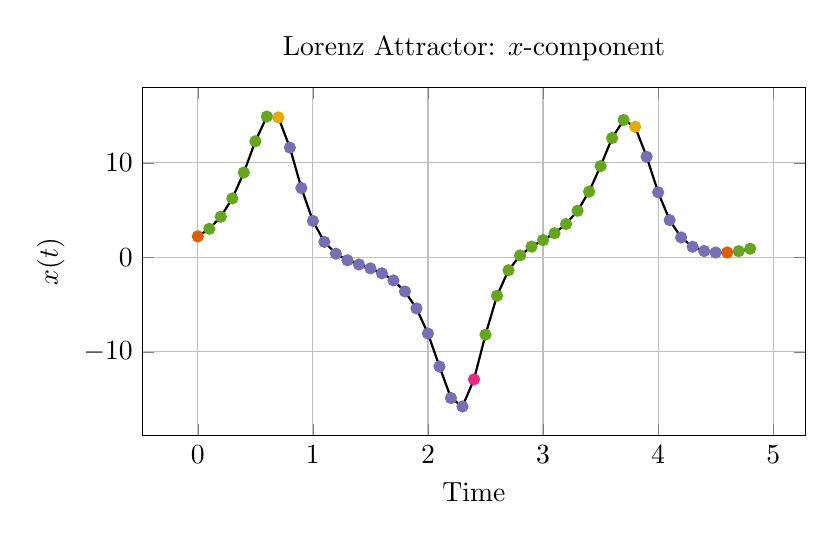
\begin{tikzpicture}
    \begin{axis}[
        xlabel={Time},
        ylabel={$x(t)$},
        title={Lorenz Attractor: $x$-component},
        width=10cm, height=6cm,
        grid=major
    ]


    \addplot [
        thick, % or any style you like
    ] coordinates {
        (0.0, 2.2165566502619796)
        (0.1, 3.0181360987381685)
        (0.2, 4.2948078524935065)
        (0.3, 6.231121537780632)
        (0.4, 8.970926893912857)
        (0.5, 12.272230400810887)
        (0.6, 14.887997312478161)
        (0.7, 14.803117347063516)
        (0.8, 11.606868473299526)
        (0.9, 7.330990437181266)
        (1.0, 3.85191889651296)
        (1.1, 1.6347534154776406)
        (1.2, 0.3853895148599277)
        (1.3, -0.30838099414996695)
        (1.4, -0.7586726217449103)
        (1.5, -1.1695821908357407)
        (1.6, -1.6858338981790886)
        (1.7, -2.443141458426554)
        (1.8, -3.6086854451117074)
        (1.9, -5.40339197322587)
        (2.0, -8.058505977971057)
        (2.1, -11.547145254692042)
        (2.2, -14.884182443761347)
        (2.3, -15.775516623377253)
        (2.4, -12.908181797239536)
        (2.5, -8.181376578133673)
        (2.6, -4.06724026097539)
        (2.7, -1.3665393788429014)
        (2.8, 0.20110496364168012)
        (2.9, 1.1324784341364973)
        (3.0, 1.8245674314417792)
        (3.1, 2.5516132966355554)
        (3.2, 3.5214281335608555)
        (3.3, 4.926987945369609)
        (3.4, 6.951562500713474)
        (3.5, 9.654345729238477)
        (3.6, 12.617195234374243)
        (3.7, 14.521825487882024)
        (3.8, 13.806356286601272)
        (3.9, 10.64113968132102)
        (4.0, 6.880279139891668)
        (4.1, 3.9367704788159394)
        (4.2, 2.1029851064946445)
        (4.3, 1.121305395878461)
        (4.4, 0.665491176850325)
        (4.5, 0.5051437108082056)
        (4.6, 0.5156168027361644)
        (4.7, 0.6490783162490397)
        (4.8, 0.9105168761220792)
    };
    
    
    % Define how each "class" (symbolic label) is colored and drawn:
    \addplot[
        scatter,
        only marks,
        scatter src=explicit symbolic,
        scatter/classes={
            1={mark=*,draw=col1,fill=col1},
            2={mark=*,draw=col2,fill=col2},
            3={mark=*,draw=col3,fill=col3},
            4={mark=*,draw=col4,fill=col4},
            5={mark=*,draw=col5,fill=col5},
            6={mark=*,draw=col6,fill=col6}
        }
    ] 
    coordinates {
        (0.0, 2.2165566502619796)[2]
        (0.1, 3.0181360987381685)[5]
        (0.2, 4.2948078524935065)[5]
        (0.3, 6.231121537780632)[5]
        (0.4, 8.970926893912857)[5]
        (0.5, 12.272230400810887)[5]
        (0.6, 14.887997312478161)[5]
        (0.7, 14.803117347063516)[6]
        (0.8, 11.606868473299526)[1]
        (0.9, 7.330990437181266)[1]
        (1.0, 3.85191889651296)[1]
        (1.1, 1.6347534154776406)[1]
        (1.2, 0.3853895148599277)[1]
        (1.3, -0.30838099414996695)[1]
        (1.4, -0.7586726217449103)[1]
        (1.5, -1.1695821908357407)[1]
        (1.6, -1.6858338981790886)[1]
        (1.7, -2.443141458426554)[1]
        (1.8, -3.6086854451117074)[1]
        (1.9, -5.40339197322587)[1]
        (2.0, -8.058505977971057)[1]
        (2.1, -11.547145254692042)[1]
        (2.2, -14.884182443761347)[1]
        (2.3, -15.775516623377253)[1]
        (2.4, -12.908181797239536)[4]
        (2.5, -8.181376578133673)[5]
        (2.6, -4.06724026097539)[5]
        (2.7, -1.3665393788429014)[5]
        (2.8, 0.20110496364168012)[5]
        (2.9, 1.1324784341364973)[5]
        (3.0, 1.8245674314417792)[5]
        (3.1, 2.5516132966355554)[5]
        (3.2, 3.5214281335608555)[5]
        (3.3, 4.926987945369609)[5]
        (3.4, 6.951562500713474)[5]
        (3.5, 9.654345729238477)[5]
        (3.6, 12.617195234374243)[5]
        (3.7, 14.521825487882024)[5]
        (3.8, 13.806356286601272)[6]
        (3.9, 10.64113968132102)[1]
        (4.0, 6.880279139891668)[1]
        (4.1, 3.9367704788159394)[1]
        (4.2, 2.1029851064946445)[1]
        (4.3, 1.121305395878461)[1]
        (4.4, 0.665491176850325)[1]
        (4.5, 0.5051437108082056)[1]
        (4.6, 0.5156168027361644)[2]
        (4.7, 0.6490783162490397)[5]
        (4.8, 0.9105168761220792)[5]
    };
    
    \end{axis}
    \end{tikzpicture}
    \caption{this is the caption}
    \label{fig:labelhere}
\end{figure}

\begin{table}[]
    \centering
    \begin{tabular}{c|cccccc}
        & \tikz\draw[fill=col1,draw=col1] (0,0) circle (0.9ex); 
        & \tikz\draw[fill=col2,draw=col2] (0,0) circle (0.9ex); 
        & \tikz\draw[fill=col3,draw=col3] (0,0) circle (0.9ex); 
        & \tikz\draw[fill=col4,draw=col4] (0,0) circle (0.9ex); 
        & \tikz\draw[fill=col5,draw=col5] (0,0) circle (0.9ex); 
        & \tikz\draw[fill=col6,draw=col6] (0,0) circle (0.9ex); \\ \hline
        \tikz\draw[fill=col1,draw=col1] (0,0) circle (0.9ex); & 0.7 & 0.1 & 0.1 & 0.05 & 0.05 & 0.0 \\
        \tikz\draw[fill=col2,draw=col2] (0,0) circle (0.9ex); & 0.0 & 0.0 & 0.0 & 0.0 & 0.9 & 0.1 \\
        \tikz\draw[fill=col3,draw=col3] (0,0) circle (0.9ex); & 0.7 & 0.1 & 0.1 & 0.05 & 0.05 & 0.0 \\
        \tikz\draw[fill=col4,draw=col4] (0,0) circle (0.9ex); & 0.0 & 0.0 & 0.0 & 0.0 & 0.9 & 0.1 \\
        \tikz\draw[fill=col5,draw=col5] (0,0) circle (0.9ex); & 0.0 & 0.0 & 0.0 & 0.0 & 0.9 & 0.1 \\
        \tikz\draw[fill=col6,draw=col6] (0,0) circle (0.9ex); & 0.7 & 0.05 & 0.05 & 0.05 & 0.05 & 0.1 \\
    \end{tabular}
    \caption{Transition probabilities between ordinal partitions.}
    \label{tab:transition_probabilities}
\end{table}

% !TEX root = ../HonoursThesisTemplate.tex

\chapter{Echo State Network with Ordinal Partition based readout switching}


Switch the readout ($C_{out}$) vector based on the ordinal partition.

When fitting the readout vectors, for each partition $p$:
\[
    (\mathbf{C_{out}})_p = (\mathbf{S}_p^T \mathbf{S}_p + \beta \mathbf{I}) \ \mathbf{S}_p^T \mathbf{Y}_p
\]
Where
\begin{itemize}
    \item $\mathbf{S}_p$ is $\mathbf{S}$ filtered to the states that results from data points with partition $p$. 
    \item $\mathbf{Y}_{p}$ is $\mathbf{Y}$ filtered to data points that follow immediately from data points with partition $p$.
\end{itemize}
And when infering the prediction at partition $p$:
\[
    \mathbf{y}(t) = (\mathbf{C}_{out})_{P(t)}\mathbf{s}(t)
\]
Where $P(t)$ is the partition of $x(t)$.

\begin{figure}
        
\centering
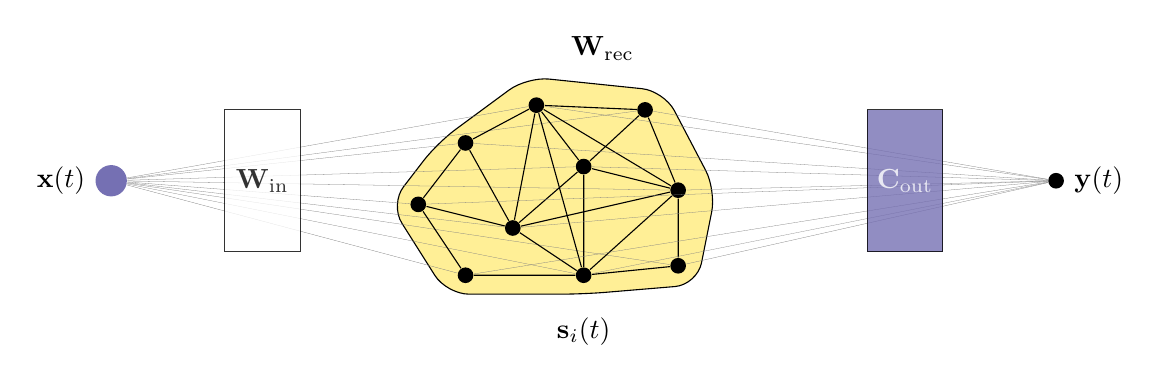
\begin{tikzpicture}[scale=1.2]
    \node[fill=col1,circle,inner sep=4pt,label=left:$\mathbf{x}(t)$] (input) at (0,0) {};
    \node[fill=black,circle,inner sep=2pt,label=right:$\mathbf{y}(t)$] (output) at (10,0) {};
    
    
    \coordinate (res_anchor) at (2,3);
    \node[fill=black,circle,inner sep=2pt] (res1) at ({5-0.5},{0.8}) {};
    \node[fill=black,circle,inner sep=2pt] (res2) at ({5},{-1}) {};
    \node[fill=black,circle,inner sep=2pt] (res3) at ({5},{0.15}) {};
    \node[fill=black,circle,inner sep=2pt] (res4) at ({5+1},{-0.1}) {};
    \node[fill=black,circle,inner sep=2pt] (res5) at ({5-0.75},{-0.5}) {};
    \node[fill=black,circle,inner sep=2pt] (res6) at ({5-1.25},{0.4}) {};
    \node[fill=black,circle,inner sep=2pt] (res7) at ({5+0.65},{0.75}) {};
    \node[fill=black,circle,inner sep=2pt] (res8) at ({5+1},{-0.9}) {};
    \node[fill=black,circle,inner sep=2pt] (res9) at ({5-1.25},{-1}) {};
    \node[fill=black,circle,inner sep=2pt] (res10) at ({5-1.75},{-0.25}) {};

    \foreach \i in {1,...,10}
        \draw[gray,line width=0.1] (input) -- (res\i);
    
    \foreach \i in {1,...,5}
        \foreach \j in {1,...,5} {
            \ifnum\i<\j
                \draw (res\i) -- (res\j);
            \fi
        }
    
    \draw (res6) -- (res5);
    \draw (res6) -- (res1);
    \draw (res6) -- (res10);
    \draw (res10) -- (res5);
    \draw (res9) -- (res10);
    \draw (res9) -- (res2);
    \draw (res7) -- (res1);
    \draw (res7) -- (res3);
    \draw (res7) -- (res4);
    \draw (res8) -- (res4);
    \draw (res8) -- (res2);
    
    \foreach \i in {1,...,10}
        \draw[gray,line width=0.1] (res\i) -- (output);
    
    \begin{scope}[on background layer]
    \draw[draw=black,fill=pale_yellow,rounded corners=8pt]  ($(res1)+(-0.1,0.3)$) -- ($(res7)+(+0.2,+0.2)$) -- ($(res4)+(0.4,0)$) -- ($(res8)+(0.2,-0.2)$) -- ($(res2)+(0,-0.2)$) -- ($(res9)+(-0.2,-0.2)$) -- ($(res10)+(-0.3,0)$) -- ($(res6)+(-0.3,0)$) -- cycle;
    \end{scope}
    \node at (5.2, 1.4) {$\mathbf{W}_{\text{rec}}$};
    \node at (5, -1.6) {$\mathbf{s}_i(t)$};
    
    \draw[fill=white,opacity=0.8] (1.2,-0.75) rectangle (2.0,0.75) node[midway] {$\mathbf{W}_{\text{in}}$};
    \draw[fill=col1,opacity=0.8] (8, -0.75) rectangle (8.8,0.75) node[midway, text=white] {$\mathbf{C}_{\text{out}}$};
\end{tikzpicture}

    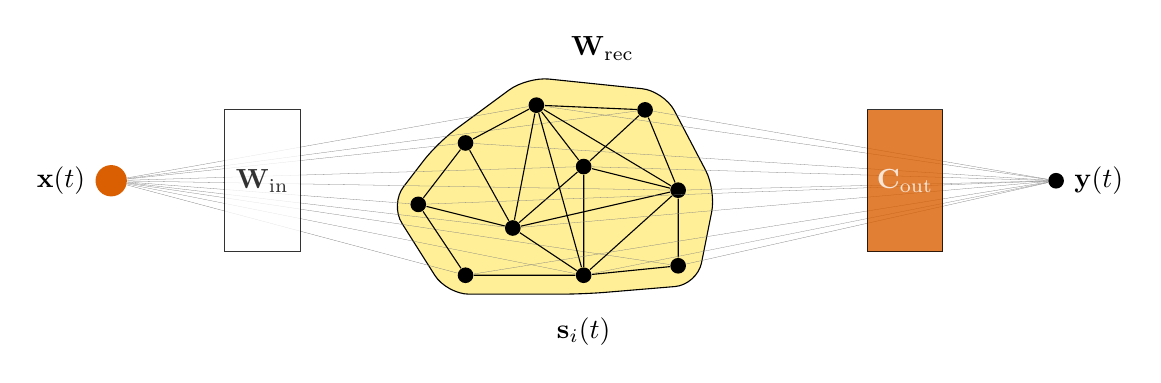
\begin{tikzpicture}[scale=1.2]
        \node[fill=col2,circle,inner sep=4pt,label=left:$\mathbf{x}(t)$] (input) at (0,0) {};
        \node[fill=black,circle,inner sep=2pt,label=right:$\mathbf{y}(t)$] (output) at (10,0) {};
        
        
        \coordinate (res_anchor) at (2,3);
        \node[fill=black,circle,inner sep=2pt] (res1) at ({5-0.5},{0.8}) {};
        \node[fill=black,circle,inner sep=2pt] (res2) at ({5},{-1}) {};
        \node[fill=black,circle,inner sep=2pt] (res3) at ({5},{0.15}) {};
        \node[fill=black,circle,inner sep=2pt] (res4) at ({5+1},{-0.1}) {};
        \node[fill=black,circle,inner sep=2pt] (res5) at ({5-0.75},{-0.5}) {};
        \node[fill=black,circle,inner sep=2pt] (res6) at ({5-1.25},{0.4}) {};
        \node[fill=black,circle,inner sep=2pt] (res7) at ({5+0.65},{0.75}) {};
        \node[fill=black,circle,inner sep=2pt] (res8) at ({5+1},{-0.9}) {};
        \node[fill=black,circle,inner sep=2pt] (res9) at ({5-1.25},{-1}) {};
        \node[fill=black,circle,inner sep=2pt] (res10) at ({5-1.75},{-0.25}) {};
    
        \foreach \i in {1,...,10}
            \draw[gray,line width=0.1] (input) -- (res\i);
        
        \foreach \i in {1,...,5}
            \foreach \j in {1,...,5} {
                \ifnum\i<\j
                    \draw (res\i) -- (res\j);
                \fi
            }
        
        \draw (res6) -- (res5);
        \draw (res6) -- (res1);
        \draw (res6) -- (res10);
        \draw (res10) -- (res5);
        \draw (res9) -- (res10);
        \draw (res9) -- (res2);
        \draw (res7) -- (res1);
        \draw (res7) -- (res3);
        \draw (res7) -- (res4);
        \draw (res8) -- (res4);
        \draw (res8) -- (res2);
        
        \foreach \i in {1,...,10}
            \draw[gray,line width=0.1] (res\i) -- (output);
        
        \begin{scope}[on background layer]
        \draw[draw=black,fill=pale_yellow,rounded corners=8pt]  ($(res1)+(-0.1,0.3)$) -- ($(res7)+(+0.2,+0.2)$) -- ($(res4)+(0.4,0)$) -- ($(res8)+(0.2,-0.2)$) -- ($(res2)+(0,-0.2)$) -- ($(res9)+(-0.2,-0.2)$) -- ($(res10)+(-0.3,0)$) -- ($(res6)+(-0.3,0)$) -- cycle;
        \end{scope}
        \node at (5.2, 1.4) {$\mathbf{W}_{\text{rec}}$};
        \node at (5, -1.6) {$\mathbf{s}_i(t)$};
        
        \draw[fill=white,opacity=0.8] (1.2,-0.75) rectangle (2.0,0.75) node[midway] {$\mathbf{W}_{\text{in}}$};
        \draw[fill=col2,opacity=0.8] (8, -0.75) rectangle (8.8,0.75) node[midway, text=white] {$\mathbf{C}_{\text{out}}$};
    \end{tikzpicture}
    \caption{Echo State Network with readout switching.}
    \label{fig:ESN}
\end{figure}
% !TEX root = ../HonoursThesis.tex

\renewcommand{\chapterlabel}{Chapter}
\chapter{Testing methods}
\label{chap:testing_methods}

\subsection{Prediction and error}

To evaluate each proposed architecture, we tested its ability to predict multiple steps of a time series and measured the resulting degree of error. The predictions take two forms: iterative prediction (a.k.a. generative, closed-loop) and direct prediction (a.k.a. teacher forced, open-loop)~\cite{lukosevicius_2012_practical_guide}. \textbf{Iterative prediction} has the readout of the ESN fitted to predict a single step into the future, and the predicted output is used as the input to derive a prediction for the following time step. \textbf{Direct prediction} has the ESN predict $n$ time steps in advance in a single shot. This can be achieved by fitting a readout matrix rather than a readout vector to predict a vector of values rather than a single value. Each of the values in the vector represent the prediction for a different value of $n$ time steps into the future. The two types of multi-step prediction are visualised in the diagrams in Figure \ref{fig:iterative_vs_direct_prediction}.
% \begin{figure}[h]
%     \centering
%     \begin{subfigure}[b]{\textwidth}
%         \centering
%         \begin{tikzpicture}
%             % Dashed lines for time steps
%             \draw[dashed] (1.5, 3.5) -- (1.5, 6.5);
%             \draw[dashed] (4.5, 3.5) -- (4.5, 6.5);
%             \draw[dashed] (7.5, 3.5) -- (7.5, 6.5);
%             \draw[dashed] (10.5, 3.5) -- (10.5, 6.5);

%             % Iterative Prediction
%             % Time series line
%             \draw[thick] (0, 4) -- (12, 4);
%             \foreach \x in {0, 3, 6, 9, 12} {
%                 \filldraw[col2] (\x, 4) circle (2pt);
%             }
%             \filldraw (0, 4) circle (2pt); % First point in black
            
%             % ESN boxes and arrows
%             \node[draw, minimum width=1cm, minimum height=0.5cm] (esn1) at (0, 6) {ESN};
%             \node[draw, minimum width=1cm, minimum height=0.5cm] (esn2) at (3, 6) {ESN};
%             \node[draw, minimum width=1cm, minimum height=0.5cm] (esn3) at (6, 6) {ESN};
%             \node[draw, minimum width=1cm, minimum height=0.5cm] (esn4) at (9, 6) {ESN};

%             \draw[->] (esn1.east) -- (esn2.west) node[midway, above] {states};
%             \draw[->] (esn2.east) -- (esn3.west) node[midway, above] { };
%             \draw[->] (esn3.east) -- (esn4.west) node[midway, above] { };
            
%             \draw[->] (0, 4.1) -- (esn1) node[midway, left] {input};
%             \draw[->] (3, 4.1) -- (esn2);
%             \draw[->] (6, 4.1) -- (esn3);
%             \draw[->] (9, 4.1) -- (esn4);
            
%             \draw[->] (esn1) -- (3, 4.1) node[midway, midway, fill=white, fill opacity=0.8, text opacity=1] {output};
%             \draw[->] (esn2) -- (6, 4.1);
%             \draw[->] (esn3) -- (9, 4.1);
%             \draw[->] (esn4) -- (12, 4.1);

%             % time step labels
%             \node at (0, 3.5) {$t$};
%             \node at (3, 3.5) {$t+1$};
%             \node at (6, 3.5) {$t+2$};
%             \node at (9, 3.5) {$t+3$};
%             \node at (12, 3.5) {$t+4$};
%         \end{tikzpicture}
%         \caption{Iterative Prediction.}
%     \end{subfigure}
    
%     \vspace{0.3cm} % Adjust vertical spacing between subfigures
    
%     \begin{subfigure}[b]{\textwidth}
%         \centering
%         \begin{tikzpicture}
%             % Direct Prediction
%             % Time series line
%             \draw[thick] (0, 0) -- (12, 0);
%             \foreach \x in {0, 3, 6, 9, 12} {
%                 \filldraw[col2] (\x, 0) circle (2pt);
%             }
%             \filldraw (0, 0) circle (2pt); % First point in black
            
%             % ESN box and arrow
%             \node[draw, minimum width=1cm, minimum height=0.5cm] (esn5) at (0, 2) {ESN};
            
%             % \draw[->] (0, 0.1) -- (esn5) node[midway, left] {input};
%             % \draw[->] (esn5) -- (2, 0.1);
%             % \draw[->] (esn5) -- (4, 0.1);
%             % \draw[->] (esn5) -- (6, 0.1);
%             % \draw[->] (esn5) -- (8, 0.1);
%             % \draw[->] (esn5) -- (10, 0.1);
%             % \draw[->] (esn5) -- (12, 0.1) node[midway, above] {outputs};
%             \draw[->] (0, 0.1) -- (esn5) node[midway, left] {input};
%             \draw[->] (esn5) -- (3, 0.1);
%             \draw[->] (esn5) -- (6, 0.1);
%             \draw[->] (esn5) -- (9, 0.1);
%             \draw[->] (esn5) -- (12, 0.1) node[midway, above] {outputs};

%             \node at (0, -0.4) {$t$};
%         \end{tikzpicture}
%         \caption{Direct Prediction.}
%     \end{subfigure}
%     \caption{Illustration of (a) Iterative and (b) Direct Prediction using an ESN, where the input data point is coloured black and the predictions are orange.}
%     \label{fig:iterative_vs_direct_prediction}
% \end{figure}
\begin{figure}[h]
    \centering
    \begin{subfigure}[b]{\textwidth}
        \centering
        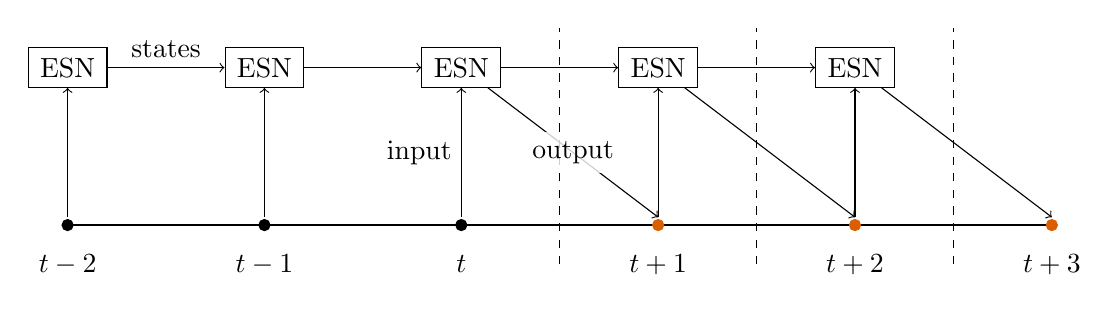
\begin{tikzpicture}
            % Dashed lines for time steps
            \draw[dashed] (1.25, 3.5) -- (1.25, 6.5);
            \draw[dashed] (3.75, 3.5) -- (3.75, 6.5);
            \draw[dashed] (6.25, 3.5) -- (6.25, 6.5);

            % Iterative Prediction
            % Time series line
            \draw[thick] (-5, 4) -- (7.5, 4);
            \foreach \x in {2.5, 5, 7.5} {
                \filldraw[col2] (\x, 4) circle (2pt);
            }
            \foreach \x in {-5, -2.5, 0} {
                \filldraw (\x, 4) circle (2pt); % First point in black
            }
            
            % ESN boxes and arrows
            \node[draw, minimum width=1cm, minimum height=0.5cm] (esn-1) at (-5, 6) {ESN};
            \node[draw, minimum width=1cm, minimum height=0.5cm] (esn0) at (-2.5, 6) {ESN};
            \node[draw, minimum width=1cm, minimum height=0.5cm] (esn1) at (0, 6) {ESN};
            \node[draw, minimum width=1cm, minimum height=0.5cm] (esn2) at (2.5, 6) {ESN};
            \node[draw, minimum width=1cm, minimum height=0.5cm] (esn3) at (5, 6) {ESN};

            \draw[->] (esn-1.east) -- (esn0.west) node[midway, above] {states};
            \draw[->] (esn0.east) -- (esn1.west);
            \draw[->] (esn1.east) -- (esn2.west);
            \draw[->] (esn2.east) -- (esn3.west);
            
            \draw[->] (-5, 4.1) -- (esn-1);
            \draw[->] (-2.5, 4.1) -- (esn0);
            \draw[->] (0, 4.1) -- (esn1) node[midway, left] {input};
            \draw[->] (2.5, 4.1) -- (esn2);
            \draw[->] (5, 4.1) -- (esn3);
            
            \draw[->] (esn1) -- (2.5, 4.1) node[midway, midway, fill=white, fill opacity=0.8, text opacity=1] {output};
            \draw[->] (esn2) -- (5, 4.1);
            \draw[->] (esn3) -- (7.5, 4.1);

            % time step labels
            \node at (-5, 3.5) {$t-2$};
            \node at (-2.5, 3.5) {$t-1$};
            \node at (0, 3.5) {$t$};
            \node at (2.5, 3.5) {$t+1$};
            \node at (5, 3.5) {$t+2$};
            \node at (7.5, 3.5) {$t+3$};
        \end{tikzpicture}
        \caption{Iterative Prediction.}
    \end{subfigure}
    
    \vspace{0.3cm} % Adjust vertical spacing between subfigures
    
    \begin{subfigure}[b]{\textwidth}
        \centering
        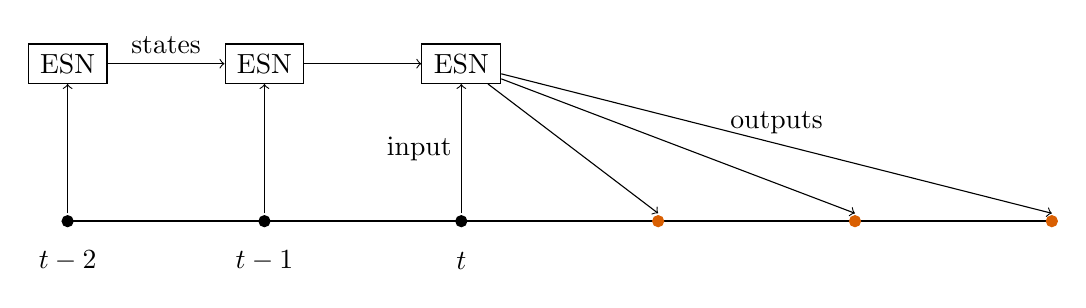
\begin{tikzpicture}
            % Direct Prediction
            % Time series line
            \draw[thick] (-5, 0) -- (7.5, 0);
            \foreach \x in {2.5, 5, 7.5} {
                \filldraw[col2] (\x, 0) circle (2pt);
            }
            \foreach \x in {-5, -2.5, 0} {
                \filldraw (\x, 0) circle (2pt); % First point in black
            }
            
            % ESN box and arrow
            \node[draw, minimum width=1cm, minimum height=0.5cm] (esn3) at (-5, 2) {ESN};
            \node[draw, minimum width=1cm, minimum height=0.5cm] (esn4) at (-2.5, 2) {ESN};
            \node[draw, minimum width=1cm, minimum height=0.5cm] (esn5) at (0, 2) {ESN};
            
            % \draw[->] (0, 0.1) -- (esn5) node[midway, left] {input};
            % \draw[->] (esn5) -- (2, 0.1);
            % \draw[->] (esn5) -- (4, 0.1);
            % \draw[->] (esn5) -- (6, 0.1);
            % \draw[->] (esn5) -- (8, 0.1);
            % \draw[->] (esn5) -- (10, 0.1);
            % \draw[->] (esn5) -- (12, 0.1) node[midway, above] {outputs};

            \draw[->] (-5, 0.1) -- (esn3);
            \draw[->] (-2.5, 0.1) -- (esn4);
            \draw[->] (0, 0.1) -- (esn5) node[midway, left] {input};

            \draw[->] (esn3) -- (esn4) node[midway, above] {states};
            \draw[->] (esn4) -- (esn5);

            \draw[->] (esn5) -- (2.5, 0.1);
            \draw[->] (esn5) -- (5, 0.1);
            \draw[->] (esn5) -- (7.5, 0.1) node[midway, above] {outputs};

            \node at (-5, -0.5) {$t-2$};
            \node at (-2.5, -0.5) {$t-1$};
            \node at (0, -0.5) {$t$};
            % \node at (2.5, -0.5) {$t+1$};
            % \node at (5, -0.5) {$t+2$};
            % \node at (7.5, -0.5) {$t+3$};
        \end{tikzpicture}
        \caption{Direct Prediction.}
    \end{subfigure}
    \caption{Illustration of (a) Iterative and (b) Direct Prediction using an ESN, where the input data points are coloured black and the predictions are orange.}
    \label{fig:iterative_vs_direct_prediction}
\end{figure}

To test the ability for an architecture to perform multi-step prediction, we will split the time series into non-overlapping chunks and perform multi-step predictions from the beginning of each chunk. For recursive predictions, the ESN will change from being driven by the true signal to being driven by its own predictions at the start of each chunk. For direct predictions, all of the values within the chunk will be predicted in one shot after being driven by the true signal up to the start of the chunk. Concatenating each of these chunks will produce discontinuous predictions over the whole time series. To achieve this, we first feed the time series into the ESN and collect the reservoir states at each time step. To generate the predictions for each chunk, we look up the reservoir state at the beginning of the chunk from the collected reservoir states. We then derive predictions for the length of the chunk starting from this state by iterative or direct prediction, yielding a series of predictions $\mathbf{\hat y}$. An example of a true time series $\mathbf{y}$ and a predicted time series $\mathbf{\hat y}$ are shown in Figure \ref{fig:predicted_chunks}. Comparing these predictions with the true values, we can calculate the Root Mean Squared Error (RMSE):
\[
  \mathrm{RMSE}
  = \sqrt{\frac{1}{n}\sum_{i=1}^n \bigl(y_i - \hat y_i\bigr)^2}.
\]

% In the time series that we measured, most of the data points belong to either the monotonically increasing partition or the monotonically decreasing partition, making the other partitions rarer - these being the `turning partitions'. To calculate the error of just these rare turning partitions, we can calculate the `turning partition RMSE', which uses the same calculation as the RMSE but filters the time steps to those in which the true values belong to a turning partition.

Using prediction error metrics such as RMSE provide a quantified means to compare the efficacy of different ESN architectures and parameter settings. Although some measurements such as memory capacity are helpful, prediction error directly reflects how well a model accomplishes the task of forecasting future time series values. A lower error signifies a more accurate prediction, indicating that the model has more effectively captured the underlying dynamics of the data. RMSE represents an average magnitude of prediction error but penalizes larger errors more heavily due to the squaring operation, making it sensitive to both the magnitude of error and the variance of the predictions.

\begin{figure}[h]
    \centering
    \begin{tikzpicture}
        \begin{axis}[
            width=\textwidth,
            height=0.3\textheight,
            xlabel={Time step},
            ylabel={x component},
            grid=major,
            grid style={gray!30, dashed},
            tick align=outside,
            xmajorgrids=true,
            ymajorgrids=true,
            legend pos=north east,
        ]
        % first series
        \addplot [col1, thick] table[
            x expr=\coordindex+1,
            y index=0
        ] {
            -7.396096508092025
            -6.861331452241957
            -6.24654642613075
            -5.556343142660912
            -4.7961801092973175
            -3.9723348591387153
            -3.091859713872994
            -2.1625265510299285
            -1.1927661001233658
            -0.19159961726161312
            0.8314359764321038
            1.8663640388207898
            2.902850544865883
            3.930278123170828
            4.937817917547159
            5.914477090775335
            6.849114329620174
            7.730377011479792
            8.546512406014008
            9.28491042719792
            9.931166901880726
            10.467234387508439
            10.867939442332478
            11.09484842529874
            11.086818184172397
            10.749857288233814
            9.959891086802305
            8.611072281223342
            6.733929065667193
            4.598225909057093
            2.6112708460638716
            1.0530118737483842
            -0.04073289738452005
            -0.7791799105487875
            -1.2910168864683638
            -1.6704435463260245
            -1.9735024345377865
            -2.2295816785884504
            -2.45248938034873
            -2.647773504057217
            -2.8169031591342404
            -2.959480280931587
            -3.0743560044046303
            -3.1601780018798156
            -3.2156556794885813
            -3.2396897286316
            -3.231437979141229
            -3.190351028531407
            -3.116193061358003
            -3.0090545160851554
            -2.869359501636886
            -2.6978689681102233
            -2.495680153051379
            -2.2642227622022926
            -2.0052509829389584
            -1.7208331476856606
            -1.413336497683052
            -1.0854105933844524
            -0.7399651495442215
            -0.3801476675590322
            -0.009314942148778507
            0.36899438242074417
            0.7510937577818644
            1.133180382870339
            1.5113734825686167
            1.88174892738536
            2.240381097518485
            2.583378769660128
            2.906929376221273
            3.2073356131323694
            3.481059794940485
            3.7247614734047247
            3.9353395637964015
            4.109970885308872
            4.246148538980052
            4.3417199850700925
            4.394920044011022
            4.4044052458184275
            4.3692784904864626
            4.2891133199460585
            4.163965515557074
            3.994379246983481
            3.781380426142671
            3.5264615878611414
            3.2315569029221423
            2.899012712429728
            2.53155384390679
            2.1322550245866085
            1.7045120331983317
            1.252021327206582
            0.7787611148498773
            0.28897188790037365
            -0.21286213958420896
            -0.722043261783661
            -1.2336920062784342
            -1.7427886867398066
            -2.2442213721515194
            -2.732836494799075
            -3.2034925165711123
            -3.651115126027906
            -4.070752281491882
            -4.457628677447651
            -4.807198839966164
            -5.1151987208186025
            -5.377695235260869
            -5.591133359345259
            -5.752379954987815
            -5.858764076128841
            -5.908113779187988
            -5.898788501706019
            -5.829705935124233
            -5.700365218975399
            -5.510863352586611
            -5.2619066040887805
            -4.954816274764559
            -4.5915272731812
            -4.174582281223459
            -3.7071174442088095
            -3.192844540888709
            -2.6360240997472797
            -2.041435705165566
            -1.4143393984874584
            -0.7604351887311834
            -0.08581372470342866
            0.603092967255068
            1.299569859994485
            1.9966742378151108
            2.6873001371022323
            3.3642362325076225
            4.020231769653453
            4.6480520486126755
            5.240538317894463
            5.790653484179682
            6.2915260831472555
            6.736474568969565
            7.119024225965137
            7.432901648545579
            7.672025525636459
            7.830497066012714
            7.902628536831873
            7.883067784815519
            7.767096030672384
            7.551188885225362
            7.233903906095832
            6.816992583099039
            6.306448592908437
            5.712985578775046
            5.051401651420454
            4.3386752327902185
            3.5912715129376838
            2.8226666776646288
            2.0420528792880575
            1.2545753539399793
            0.46271556623987947
            -0.33195597063982063
            -1.127343523959916
            -1.920039395871976
            -2.705156513704118
            -3.476565692053726
            -4.227290068346756
            -4.949892371256707
            -5.6367813018981225
            -6.2804307728143165
            -6.873534483951402
            -7.409120531017614
            -7.880644336610527
            -8.282069850727668
            -8.607943406953376
            -8.853461720468228
            -9.014534127582214
            -9.087838667705672
            -9.070871388939759
            -8.961988455898853
            -8.760440541151308
            -8.466398241296694
            -8.080969538755438
            -7.606207995622861
            -7.045110630247198
            -6.401608561049777
            -5.680545008782908
            -4.8876470832188215
            -4.029485801668654
            -3.1134282082669555
            -2.1475816313080265
            -1.1407282361208144
            -0.10225514973422133
            0.9579231335119591
            2.0294448728455508
            3.101581632245292
            4.163317154695597
            5.2034116780830715
            6.210445563385217
            7.172808896736733
            8.07860265709465
            8.915341926839472
            9.669313064115922
            10.324208367624527
            10.858408350579182
            11.23976598986951
            11.416329857680902
            11.3024212850999
            10.766599294757865
            9.649691443890664
            7.867323652359783
            5.589884615445816
            3.2766531677329787
            1.380132785106338
            0.056232791703295024
            -0.7919100912380274
            -1.329173440294901
            -1.6857661007092588
            -1.9408479458260801
            -2.136479531206684
            -2.293081355571852
            -2.419726254719428
            -2.519922919107634
            -2.5946139366972547
            -2.643660612136656
            -2.666558489593934
            -2.6627768269967236
            -2.631919048466718
            -2.5737991854672924
            -2.48847888071175
            -2.3762852822613625
            -2.2378190267934785
            -2.07395631008147
            -1.8858466929713105
            -1.6749077365226335
            -1.4428162190079865
            -1.1914967343094078
            -0.9231074451923874
            -0.6400229205144317
            -0.3448150245563004
            -0.04023054004027646
            0.27083233086557085
            0.5853507760686197
            0.9002045646383525
            1.2122064091421454
            1.5181319384869962
            1.8147525736813077
            2.0988675683023463
            2.367337630047389
            2.6171189463074693
            2.8452953675885553
            3.0491141124096313
            3.2260149944797494
            3.373666254780228
            3.489990391252424
            3.5731968206014457
            3.621804963724474
            3.6346689692713663
            3.6109974330140577
            3.5503673403591094
            3.452736092633235
            3.318444517241951
            3.148217463161521
            2.9431562351102576
            2.704728370180026
            2.4347521091999673
            2.1353790381040616
            1.8090757246671372
            1.4586025620755936
            1.0869962668626643
            0.6975462494979143
            0.2937745111071812
            -0.12058967682017309
            -0.5416386163609112
            -0.9653158812942618
            -1.387452020442244
            -1.8038039696275774
            -2.210093923375732
            -2.60205365216642
            -2.9754681895282165
            -3.326219612454469
            -3.650331967204639
            -3.9440150937506604
            -4.203706644262557
            -4.426113390692141
            -4.60825066203126
            -4.74747843810255
            -4.8415353345492695
            -4.888569871541362
            -4.887166725504471
            -4.836370725172766
            -4.735705735217822
            -4.585188976904356
            -4.385341748961086
            -4.137193441310793
            -3.842282920291269
            -3.5026519977709363
            -3.1208368691067303
            -2.699851110584447
            -2.2431668880710833
            -1.754688120494503
            -1.2387216150963267
            -0.6999412883886329
            -0.14335016900372038
            0.42576314641813534
            1.0018703082781808
            1.5792526873399777
            2.152053255137486
            2.7143296567768975
            3.2601101868295332
            3.783447536991531
            4.278476218728446
            4.739464912022299
            5.160872062307513
            5.537396164720593
            5.864028152257837
            6.136102567125602
            6.3493512483380945
            6.4999668321516175
            6.584673428118075
            6.600824677849305
            6.546515905850497
            6.420730954965775
            6.223493621496039
            5.956011203205806
            5.620761945505625
            5.22147910802633
            4.762992287567513
            4.25093012046693
            3.6913320497845272
            3.0902647954319673
            2.4535531953552034
            1.7866924476710255
            1.0949424096470635
            0.38354089388570267
            -0.3420631973112844
            -1.076036390058153
            -1.812092711355816
            -2.5435237711179983
            -3.2632966648424535
            -3.964181413907237
            -4.638880810487975
            -5.2801485791466325
            -5.8808930584740295
            -6.434268858991435
            -6.933759884648678
            -7.373256263808548
            -7.747126499509461
            -8.050285190133012
            -8.278256102391108
            -8.427230117502384
            -8.494117535059218
            -8.476594202878472
            -8.373140439702501
            -8.183072890434062
            -7.906568977696387
            -7.544681999564055
            -7.099349145660523
            -6.573389808493353
            -5.970495152739064
            -5.295209710934485
            -4.552902111335496
            -3.7497299844550467
            -2.8925934283167685
            -1.9890830713324636
            -1.0474193338452686
            -0.07638506109284685
            0.9147452380776678
            1.916283973972553
            2.9182051741617525
            3.9102234040486903
            4.881859522196724
            5.822494774774458
            6.72138792877968
            7.567637239182163
            8.35001920711162
            9.056631446604579
            9.674139545724154
            10.186334288286341
            10.571489800501663
            10.79784514275587
            10.816822854532223
            10.555716789805897
            9.918264573337886
            8.81349110487454
            7.233093903071334
            5.340479732915809
            3.4474764819419135
            1.8376119212548883
            0.6189396449110495
            -0.25586893617059187
            -0.8900998548341339
            -1.375656479276715
            -1.7737993796270544
            -2.1192358277078944
            -2.4292164782683288
            -2.710967465708411
            -2.966446905067794
            -3.195055831155762
            -3.395080747997942
            -3.564427733274559
            -3.700987072677495
            -3.802814769266202
            -3.8682262396309017
            -3.8958489256434166
            -3.884655122010877
            -3.8339845355303175
            -3.7435605320303793
            -3.6135015293975115
            -3.444328281666954
            -3.2369670846161713
            -2.992748493350548
            -2.7134027866698682
            -2.4010500042722094
            -2.0581876032848916
            -1.6876719227136014
            -1.29269827687254
            -0.8767742721650653
            -0.4436928730676188
            0.0025016555452202142
            0.4575468083513791
            0.91700222240304
            1.3762876955259649
            1.8307285295780351
            2.275596892532985
            2.706161219182819
            3.11772879520624
            3.5056977368317
            3.8656001112348894
            4.193154513367069
            4.4843095228931835
            4.735296182478027
            4.9426719152976775
            5.103373543491249
            5.214762178749549
            5.274677081691406
            5.281480480941951
            5.234107886083136
            5.132105252992437
            4.97566073881508
            4.765616075092398
            4.503457188171087
            4.191279706976005
            3.831730710910728
            3.4279340467074726
            2.9834139070560375
            2.5020249746332817
            1.9879090104733965
            1.4454705627302449
            0.8793777547674209
            0.2945693027211369
            -0.30373998131733715
            -0.9100691130848559
            -1.5186996328918754
            -2.123722026166143
            -2.7190954467221715
            -3.2987153726282443
            -3.8564841785882673
            -4.38638168631783
            -4.882534095316639
            -5.339280736433374
            -5.751238410871965
            -6.11336314866123
            -6.421009129265768
            -6.669984409097591
            -6.856602998802089
            -6.977732553673773
            -7.030837454025051
            -7.0140168971440655
            -6.926037163929942
            -6.766357327189573
            -6.535149548123476
            -6.233311447187571
            -5.86247215926009
            -5.424991123206696
            -4.923948750389981
            -4.36313132999403
            -3.7470062309743084
            -3.080692803408184
            -2.3699230161865295
            -1.6209990941097072
            -0.8407409855931645
            -0.036432169956123424
            0.7842431486637602
            1.6132635826402173
            2.442339623764592
            3.2629812781084526
            4.066566726399407
            4.844404854718961
            5.587789258094579
            6.288036141897227
            6.936493782287796
            7.524509511606392
            8.043326445632376
            8.483882105748613
            8.836455492013261
            9.090145108849168
            9.232160781774297
            9.24708897342554
            9.116558908095724
            8.820254296014905
            8.339730045882721
            7.666265702921442
            6.811671647653022
            5.816348787533623
            4.745957839691597
            3.6735327145823176
            2.6562910249615697
            1.7219973280172574
            0.8709730216281464
            0.08769597138904799
            -0.6472167528581492
            -1.3495802959917857
            -2.02897443640829
            -2.689052669206035
            -3.32905079039029
            -3.945404863650343
            -4.5330198759879226
            -5.086113009347103
            -5.598719616734639
            -6.064982121329375
            -6.4793180232234535
            -6.836526754906759
            -7.131867759202054
            -7.361124313372444
            -7.520659172896184
            -7.607464004419815
            -7.619203005683116
            -7.554250267789292
            -7.411720748858491
            -7.191494579654525
            -6.894233849729034
            -6.5213917101450045
            -6.075214734133178
            -5.558735325652912
            -4.975759024144955
            -4.330840566562098
            -3.6292550765958644
            -2.8769594986469644
            -2.080547462445707
            -1.2471979938699036
            -0.38461584256615444
            0.49903041325790237
            1.3951789478479717
            2.294943604835933
            3.1891885497669845
            4.068597042695082
            4.92373752989793
            5.745114740473685
            6.523198676995644
            7.248411696917967
            7.911046163916741
            8.501063266250108
            9.007694533351042
            9.418743311874525
            9.719419460577367
            9.890611175874895
            9.906693848590875
            9.733739953699777
            9.33062739959564
            8.657809979470741
            7.698514296049501
            6.488233006233911
            5.129835545270621
            3.7668540273955284
            2.523353587729627
            1.4589207131761928
            0.5694842831558906
            -0.18293393324093002
            -0.8416747547789684
            -1.4407505765805022
            -2.0015259503579053
            -2.5347750580428325
            -3.0440503555743774
            -3.5285946540399498
            -3.985359644454659
            -4.410239565415787
            -4.798765571527368
            -5.146478555438499
            -5.449129081921403
            -5.702791550448796
            -5.903937727273476
            -6.0494910834822635
            -6.136871061857738
            -6.164030697835843
            -6.129488700978248
            -6.032356342304665
            -5.872358443678261
            -5.649848699763408
            -5.365819498696942
            -5.021904247598893
            -4.62037500285764
            -4.164131842502035
            -3.6566874994652516
            -3.102144100009856
            -2.505164523404777
            -1.8709376405741107
            -1.2051368260201387
            -0.5138750185158993
            0.19634803163668355
            0.9186989420084758
            1.646072460317327
            2.371149821250802
            3.0864656879788748
            3.784467644281785
            4.457581906291181
            5.098267474709328
            5.699070432608697
            6.252661025331669
            6.751861160041427
            7.189645414806263
            7.5591218273867815
            7.853480113636897
            8.065923735586868
            8.189607191046887
            8.217638920349806
            8.14326227915589
            7.960375881162427
            7.6645644522297065
            7.254701175032213
            6.734878534767123
            6.1159709094209855
            5.41576386794923
            4.656883245182037
            3.8627812889362234
            3.05330479415744
            2.241776599118178
            1.4346447937898972
            0.6333319897853195
            -0.16299723200648822
            -0.9550009007736938
            -1.7417017802725874
            -2.520039994190614
            -3.2851045815075604
            -4.030659916670965
            -4.7496908740622406
            -5.434837692032996
            -6.078699544725634
            -6.674035827160324
            -7.213903693643309
            -7.6917607535042976
            -8.101550061850963
            -8.437775280515764
            -8.695569197419344
            -8.87075636574291
            -8.959909723756658
            -8.960400589527934
            -8.870441513849558
            -8.689121626287823
            -8.416434000927534
            -8.053293615835061
            -7.601547726866943
            -7.0639759371655835
            -6.444281305938126
            -5.747072783323798
            -4.977836413027253
            -4.1429000026916105
            -3.2493862538161493
            -2.3051591049384856
            -1.3187620353375769
            -0.2993479768242967
            0.7433938781193455
            1.7993188950733492
            2.8579059857047957
            3.9083368997564794
            4.939565485468307
            5.940367229779519
            6.899349866100953
            7.804885138964935
            8.644895930044418
            9.406350605038657
            10.074215662882184
            10.629346514066054
            11.044449106822686
            11.276813825628313
            11.256884426111016
            10.87587638707581
            9.990122056567065
            8.484763547043947
            6.422647563698681
            4.149861111022549
            2.1275687501323945
            0.6176045851558069
            -0.39444589594943946
            -1.0510375940253223
            -1.4909822110010262
            -1.8074400183347457
            -2.0529257303709927
            -2.2540085600650213
            -2.4229061192111008
            -2.5645219072467094
            -2.6802619294600674
            -2.769982689477447
            -2.832949398258732
            -2.8682970378632042
            -2.875250535706721
            -2.8532306163248164
            -2.8019062429963633
            -2.721221536148972
            -2.6114099264510973
            -2.473001134966312
            -2.3068232824827835
            -2.114001280909338
            -1.8959519263604516
            -1.6543754154444636
            -1.3912445745181543
            -1.1087898630259265
            -0.809483160616639
            -0.4960166388679021
            -0.17128159051496764
            0.16165821430016905
            0.4995920297411621
            0.8391934211757658
            1.1770492962699923
            1.5096949034640157
            1.8336451544378256
            2.145432621130641
            2.4416397680314024
            2.718938673532908
            2.9741237902423237
            3.20415089411391
            3.406170972528778
            3.577565435553505
            3.7159810818088945
            3.819359756805601
            3.8859719950617198
            3.914440384308632
            3.9037671690628195
            3.8533503407045115
            3.7629994448836235
            3.6329421134679745
            3.463824653094563
            3.256706499780123
            3.013046403825484
            2.734686676392727
            2.4238302770962132
            2.083021318533591
            1.7151198701265522
            1.3232839157132956
            0.9109460654096122
            0.4817931566766648
            0.039743865446442074
            -0.4110794239917672
            -0.8663801090670229
            -1.321722892799363
            -1.7725745676517124
            -2.2143460976508176
            -2.6424386862897054
            -3.0522914715648137
            -3.439429505395385
            -3.7995115947690925
            -4.128378036086235
            -4.422097241312322
            -4.677010629159925
            -4.889775323511156
            -5.057404823321077
            -5.1773069691948725
            -5.2473178058035375
            -5.2657324617073265
            -5.2313323117293455
            -5.143406363026918
            -5.001769815291969
            -4.806775992729643
            -4.559324275987273
            -4.260862054876429
            -3.913381489723183
            -3.519410576662779
            -3.081998983579548
            -2.6046977713251107
            -2.0915347151215196
            -1.5469831703901167
            -0.9759273314707573
            -0.38362149246285643
            0.22435368778690198
            0.8421400916389513
            1.4636528710743864
            2.0826357211141415
            2.692715763176079
            3.2874629444626873
            3.860445623252189
            4.405290473670829
            4.915735636821259
            5.385686346241047
            5.809263038368363
            6.180849121113483
            6.495134681275236
            6.747159848979476
            6.932367045010044
            7.046663055628635
            7.086519065407552
            7.049107892742522
            6.932510870506065
            6.7359841821834765
            6.460260210081611
            6.107828311837552
            5.683075565053195
            5.192185200088587
            4.642719723297308
            4.042934725613215
            3.4009898862643677
            2.7242994099950555
            2.0192239221540054
            1.2911665009978717
            0.544974929780568
            -0.21454764777076968
            -0.9822151556919649
            -1.7522222729752996
            -2.518111731760845
            -3.272885422782383
            -4.009182257583405
            -4.719464648258854
            -5.396181805025817
            -6.031903919767473
            -6.619432360400211
            -7.15189348432177
            -7.622822394508429
            -8.02624005435296
            -8.35672516764257
            -8.609481065535647
            -8.78039727864807
            -8.866105288703523
            -8.86402792057296
            -8.772421418706651
            -8.590410101153171
            -8.318013306549576
            -7.956163122062785
            -7.506713747982632
            -6.972442271923079
            -6.357038502209698
            -5.6650882596181384
            -4.902044126020501
            -4.074190193058977
            -3.1885958839345467
            -2.253061922533438
            -1.2760597653571009
            -0.26666160897314867
            0.7655323228115852
            1.8104734684904424
            2.857744095376678
            3.896635253103686
            4.9162169577806525
            5.905387551940879
            6.852887828576188
            7.747238035833139
            8.576542104550526
            9.32801397442611
            9.9870063863459
            10.535065839538671
            10.946240081524294
            11.18049371409666
            11.173411288627321
            10.824928148622298
            10.002113433784274
            8.592781076587837
            6.636600553325218
            4.433381814733946
            2.4177362997471725
            0.8688021286585401
            -0.19621479450143264
            -0.9016929595340593
            -1.3824163971375998
            -1.7333667444126166
            -2.00971231670381
            -2.239927204307435
            -2.437271147179097
            -2.6070829898682466
            -2.750846456105503
            -2.8683048678127374
            -2.9585154719475497
            -3.0203618634028664
            -3.052800344150161
            -3.054979603094141
            -3.0263006333439324
            -2.9664485108802188
            -2.8754101648039545
            -2.753484374438082
            -2.6012866829311383
            -2.4197504147939632
            -2.2101238281225233
            -1.9739644008658064
            -1.7131292121840676
            -1.4297626591782522
            -1.126280597733309
            -0.8053516727068805
            -0.469875660948903
            -0.1229590098265966
            0.23211213296238614
            0.5919012319173876
            0.9528529766845553
            1.3113263416509064
            1.6636299561399326
            2.006057552602377
            2.3349264147485047
            2.6466134228041533
            2.9375960881912038
            3.204487508246936
            3.4440789743890288
            3.6533732162154373
            3.8296263357568328
            3.970379597368076
            4.073497700933891
            4.13719872095775
            4.160085102382612
            4.141169387504423
            4.079893942285346
            3.976146838640761
            3.830267081946862
            3.6430445836012053
            3.415709178217821
            3.1499146205204607
            2.8477145778507733
            2.511538421607292
            2.1441627996399264
            1.7486895208419353
            1.3285215346710975
            0.8873426349861743
            0.4290986611531567
            -0.042027539208346634
            -0.5216398010155797
            -1.0051621196141767
            -1.4878766502214658
            -1.9649653405317902
            -2.4315574028903506
            -2.8827789112047975
            -3.313803616934396
            -3.7199043768507987
            -4.096504609505318
            -4.439228852289568
            -4.743952059675206
            -5.006846823031341
            -5.224428581386037
            -5.393598278258507
            -5.511681882660716
            -5.5764658204978295
            -5.586229104904532
            -5.539771153681826
            -5.436433844062936
            -5.276120194606818
            -5.059306090971527
            -4.787047794280836
            -4.460982901506906
            -4.0833259733647544
            -3.656857989405192
            -3.184910274702364
            -2.6713421248535307
            -2.120513338847935
            -1.5372508055574223
            -0.9268100930734543
            -0.29483235396535157
            0.352703685382713
            1.0095329625874692
            1.6691593020451132
            2.3249125881913604
            2.9700082055393198
            3.5976068866054485
            4.200874202931939
            4.7730382597409164
            5.307444590027983
            5.7976048494123535
            6.2372415243321235
            6.620321746350478
            6.941089210555457
            7.194086634304772
            7.37419121435758
            7.476664841799803
            7.497260159462166
            7.432413246431775
            7.27955438535331
            7.0375768156854965
            6.707400761142245
            6.292523323665984
            5.799336112839675
            5.23695052483962
            4.616398637641727
            3.949315100701007
            3.246490008130999
            2.5167985932281325
            1.7668566298448958
            1.0014280137895435
            0.22429683698222688
            -0.5607979566415261
            -1.3494784701722933
            -2.1364188248352214
            -2.915360063487481
            -3.6793193198766363
            -4.420860616070394
            -5.132346813612325
            -5.806140754857656
            -6.434758019572599
            -7.010984663262542
            -7.527974039673608
            -7.979331453358625
            -8.359191321879802
            -8.662288647700974
            -8.884025103075558
            -9.020529436418183
            -9.06871157659954
            -9.026309822405107
            -8.891930628719624
            -8.66508073896938
            -8.346190197700059
            -7.936626963051646
            -7.438702952982263
            -6.855668843128395
            -6.191702392607251
            -5.4518838046669895
            -4.642164746147486
            -3.7693263791194025
        };
        \addlegendentry{True values}

        % second series
        \addplot [col2, thick, dashed, mark=*, mark repeat=101] table[
            x expr=\coordindex+1,
            y index=0
        ] {
            % (the same sequence of values as before; unmodified)
            -7.22737835401972
            -6.7170191564231345
            -6.227298531377528
            -5.633061313786811
            -4.9512351770531495
            -4.206576455136201
            -3.427168935011423
            -2.552564392838349
            -1.67589371567135
            -0.7913787358413629
            0.07621126036877968
            0.9509726816996817
            1.8328892903645624
            2.7039934227094022
            3.5208534699998495
            4.267796382884342
            4.979816181912497
            5.704664152647695
            6.437336853627357
            7.139733669455211
            7.783025230180954
            8.349807153784809
            8.83188506513602
            9.227039710516635
            9.53023164869245
            9.7281704915398
            9.802333395177754
            9.732343370791398
            9.49855798502989
            9.082907725123164
            8.467486666180662
            7.636388233334685
            6.593304078190613
            5.401553913598093
            4.190273979772201
            3.0435448936364082
            1.9428155232881181
            0.8938817053893331
            -0.0162020500916924
            -0.7575244187402177
            -1.393622108279601
            -1.959725334927839
            -2.4692248487315283
            -2.9246629603362635
            -3.331543845316105
            -3.689841755721318
            -3.9992572545844496
            -4.262477002787364
            -4.481540425333833
            -4.658650011828968
            -4.794888818373465
            -4.891719720195624
            -4.9496983662644425
            -4.969263891160381
            -4.9504179017822025
            -4.892960182675438
            -4.796364304341523
            -4.659856851827044
            -4.482532476181632
            -4.263488371444851
            -4.002246014619459
            -3.6992881749597473
            -3.3568768604568504
            -2.9797753902169006
            -2.5755564883338593
            -2.153866408855947
            -1.7245396136352156
            -1.2951388211488393
            -0.8690213918270615
            -0.4446734948739959
            -0.01636390442757829
            0.4240828268677319
            0.8844941266850128
            1.3687252680621782
            1.8732157881390208
            2.3861766117549337
            2.892045756084542
            3.3799474733885972
            3.8491480661445507
            4.305608886536447
            4.753522727621316
            5.1909889952317485
            5.611225263943481
            6.004171782501203
            6.357394100257352
            6.657949569229402
            6.894278423599133
            7.0567181443629465
            7.137029281615241
            7.127828871762517
            7.02241054406943
            6.81526521543384
            6.503522644841155
            6.08915032885443
            5.580886378814341
            4.993810563197087
            4.345091155623265
            3.6485480605342104
            2.914104489817703
            2.154620597322946
        };
        \addplot [col2, thick, dashed, mark=*, mark repeat=101] table[
            x expr=\coordindex+101,
            y index=0
        ] {
            -4.046409638877208
            -4.249441910525775
            -4.386355294100554
            -4.488465167465847
            -4.577575192342124
            -4.615412176849418
            -4.596761181713873
            -4.5607838844712205
            -4.470566182629227
            -4.347959531792526
            -4.177549506853211
            -3.972330140413078
            -3.7224768849929433
            -3.435684974948458
            -3.113127554235689
            -2.7610885559814733
            -2.3876738824963013
            -2.001009562198192
            -1.610225971111504
            -1.2201440616477157
            -0.8334720678805638
            -0.44779795854714166
            -0.05803262341305526
            0.34336276687895406
            0.7636731763361695
            1.2074972046631274
            1.6737053442706156
            2.153929973701736
            2.634610815238318
            3.103066798142436
            3.5537698400893873
            3.9889223884929947
            4.41284780332046
            4.826372480197449
            5.225776308646289
            5.603997883915156
            5.95136548199855
            6.2565478104569365
            6.508154591697348
            6.6959077008907
            6.810930264343767
            6.8455806161488795
            6.793293517141308
            6.648771652551204
            6.408778134191664
            6.073503901504125
            5.647962917954942
            5.142237493902655
            4.5694254835141805
            3.9419650577856373
            3.2696109238751774
            2.562147601199797
            1.836355086546689
            1.1218595008883199
            0.4547921767646699
            -0.14404180025820779
            -0.6800417313006619
            -1.1692317528309673
            -1.6239031274585045
            -2.049797667805592
            -2.4471479434711227
            -2.812174948191796
            -3.13974072652843
            -3.426127910009882
            -3.669696794602487
            -3.870230740779334
            -4.028151455041211
            -4.144138231126021
            -4.218868829386452
            -4.2528634139044925
            -4.2464489777280505
            -4.199785325985204
            -4.112936503307196
            -3.985998079396495
            -3.8193185396357876
            -3.61381322154557
            -3.3713704640654214
            -3.095277425362383
            -2.7905118125404442
            -2.4636715040305717
            -2.1223582706691104
            -1.7740402485283084
            -1.4247054472629088
            -1.0777568411699576
            -0.7334633559921713
            -0.3890266795622779
            -0.039178009102101896
            0.32276143945568947
            0.703339619955841
            1.1069397563131247
            1.5335216010586237
            1.97708112809471
            2.426425129981965
            2.8691868826670657
            3.297222181439963
            3.709090816410651
            4.107358954192932
            4.493759271613726
            4.866738553701623
            5.221707752759016
            };
            \addplot [col2, thick, dashed, mark=*, mark repeat=101] table[
                x expr=\coordindex+201,
                y index=0
            ] {
            10.644331104260516
            9.623557383533694
            8.081276536972268
            6.042793830399603
            3.8653321558816742
            2.143039211412429
            0.9346532073040521
            -0.12808019517422053
            -1.0558826729165958
            -1.7546047174212163
            -2.370164004031551
            -2.9037973110122266
            -3.3874848230387897
            -3.80088369056557
            -4.167622001740028
            -4.487796673775506
            -4.761782149640794
            -4.995519886577313
            -5.188669108286831
            -5.345105563271545
            -5.462800897933221
            -5.544469260457163
            -5.588855206694234
            -5.596886558217079
            -5.5678969677790064
            -5.501989050571638
            -5.398567008973032
            -5.256898258970523
            -5.075977696500786
            -4.8543062085434485
            -4.590321396505487
            -4.2824193248411575
            -3.9299454698629006
            -3.5340220054492875
            -3.098989179755449
            -2.63304369920354
            -2.1476028619417775
            -1.6545681064405926
            -1.1626233898863916
            -0.6745140991329208
            -0.1865948864435154
            0.309412683983453
            0.8229166078834282
            1.3595091894673033
            1.9159387999756063
            2.478543472023091
            3.029231423819283
            3.5570884366232463
            4.064905999769337
            4.56252373826851
            5.054622567924241
            5.536729688099001
            5.99866881269395
            6.426933474688099
            6.8062455077702
            7.12258487865455
            7.365033184450567
            7.525053977301354
            7.594987247669053
            7.567122118095028
            7.433508783765717
            7.1866947118154485
            6.8217783097904885
            6.33992668478345
            5.7522325400164505
            5.080165713867473
            4.348622870645272
            3.5757124398684255
            2.7718425484101203
            1.9518031518472299
            1.1481164387568015
            0.40652464437124536
            -0.2462747646982848
            -0.8211931171334754
            -1.3406736274183686
            -1.8190875730928724
            -2.26215417990295
            -2.67014654645277
            -3.0398429224488837
            -3.3671997566252685
            -3.650191183783477
            -3.8886628973318693
            -4.083379834890707
            -4.235300658208416
            -4.345423001153108
            -4.414562796373502
            -4.4432509482890055
            -4.431751103558781
            -4.3800925374430335
            -4.288134949705864
            -4.155676734927283
            -3.982669043099918
            -3.7695237052141692
            -3.517556420748633
            -3.2295025733678813
            -2.909961910222023
            -2.565498130040396
            -2.204117277790374
            -1.8340521547468143
            -1.4621635629424645
            };
            \addplot [col2, thick, dashed, mark=*, mark repeat=101] table[
                x expr=\coordindex+301,
                y index=0
            ] {
            2.3003873898896927
            2.799101636581838
            3.2506751610215474
            3.651278747530341
            4.1327402347063185
            4.5477124275152505
            4.954629473880686
            5.354626076660111
            5.731467114861971
            6.071707927174543
            6.36245545082113
            6.60246191084309
            6.770996356599028
            6.865629931693093
            6.876254711569288
            6.798386303953862
            6.625722559688882
            6.356242444078987
            5.99137269590301
            5.537474171161705
            5.006301632848533
            4.411401560727768
            3.7650104884306757
            3.0763984743539368
            2.356648316319024
            1.6259932433617337
            0.9178053898458529
            0.2666466764646316
            -0.3145908272508109
            -0.8369474936650931
            -1.3164246991685786
            -1.763431736663449
            -2.1819197174376654
            -2.570740869648489
            -2.925389101530527
            -3.2409930297301344
            -3.5145614210564418
            -3.7450417491243115
            -3.932522831866436
            -4.077557495239148
            -4.180868111343557
            -4.243100906280574
            -4.264720178382731
            -4.245993819704836
            -4.187036486198394
            -4.087892315529871
            -3.9486883720209107
            -3.769883581855197
            -3.55261285250981
            -3.299113874316504
            -3.0131386009435346
            -2.700169876040036
            -2.367206920926037
            -2.021978092630661
            -1.671688563042835
            -1.3216863033696313
            -0.9744893116673552
            -0.6294183945893224
            -0.28283473657216973
            0.07111309339217087
            0.43927498207943927
            0.8277861496029004
            1.2398922552603153
            1.6737586016604382
            2.121472273401423
            2.5708538210794813
            3.010315378618543
            3.4338434308360775
            3.8418247082807397
            4.237078569169569
            4.620389680665198
            4.98912441559213
            5.337834700279529
            5.658782296467962
            5.942545378757586
            6.179120532182253
            6.3589486339648715
            6.47345429456891
            6.515232080443752
            6.4781284884142
            6.357458774898589
            6.150552867139538
            5.857602016849455
            5.482416044063939
            5.0323851842438785
            4.517093004854132
            3.946081127107334
            3.327630417862565
            2.6705000338623677
            1.9888495213538704
            1.3073297770259842
            0.658448098125973
            0.06660097891693795
            -0.4658764282203265
            -0.9512796224878457
            -1.4022250751116303
            -1.8261432837787765
            -2.2249396726170403
            -2.5959142426435164
            -2.933792136375814
            };
            \addplot [col2, thick, dashed, mark=*, mark repeat=101] table[
                x expr=\coordindex+401,
                y index=0
            ] {
            -3.667128787876095
            -3.5230927210011487
            -3.341941795086086
            -3.1234703155015495
            -2.87152466752741
            -2.599344998507263
            -2.3126803243480936
            -2.0090398178442683
            -1.705076130641146
            -1.398277353161859
            -1.0954402495004274
            -0.7940277479290785
            -0.4937580634229448
            -0.18949331602760822
            0.12391228272173294
            0.45239233703205173
            0.8011976868351098
            1.1730023903790538
            1.5667287619143622
            1.976153493812717
            2.3912097483016055
            2.8009259071208135
            3.197718066723553
            3.579137576705591
            3.9461697482852856
            4.299694123098334
            4.638478503908118
            4.959005672875492
            5.255835331274284
            5.521918684683385
            5.749204206152228
            5.929419007391914
            6.054695563849009
            6.117991164379077
            6.113371256089749
            6.036264376020938
            5.883793295776343
            5.655214297847806
            5.352296968398434
            4.9793176944034485
            4.542390701312911
            4.048294513429084
            3.503618833335281
            2.91539222611965
            2.29388512930376
            1.6567211118393743
            1.0301970465153545
            0.4415623283307468
            -0.09519072188061273
            -0.5835788263701147
            -1.0347780277790548
            -1.4584981325724016
            -1.8598994611502349
            -2.2392411316704397
            -2.59269880850934
            -2.9145895986798678
            -3.1998901546489833
            -3.44543581787309
            -3.6497858133900536
            -3.8125704093026798
            -3.9339743549600144
            -4.014401056542738
            -4.0542713452883845
            -4.053934467169711
            -4.013669353987893
            -3.933751645673624
            -3.81458568625078
            -3.656918293565923
            -3.4621316042006356
            -3.232589809242995
            -2.971960061594359
            -2.6853669365679025
            -2.3792079773782007
            -2.06052628728537
            -1.7360148294881128
            -1.4109237833526436
            -1.0882027768064972
            -0.7680872510942436
            -0.4481557635369313
            -0.12378630727170048
            0.21104448407959353
            0.5626047415472613
            0.9358440228581344
            1.3325030158409845
            1.7494046064857685
            2.1780646730920807
            2.606855045171187
            3.025447472908411
            3.4287181975819294
            3.816840884168016
            4.191734147637874
            4.553550434911244
            4.899664888262748
            5.225085386524711
            5.522833953102122
            5.784468083776233
            6.000970487997961
            6.1635879962970535
            6.2643553791860995
            6.296382535056466
            };
            \addplot [col2, thick, dashed, mark=*, mark repeat=101] table[
                x expr=\coordindex+501,
                y index=0
            ] {
            2.169612500669757
            1.3182769248876411
            0.5289395497201212
            -0.19135099159564106
            -0.8231118395863746
            -1.4253303153876686
            -1.877115791444055
            -2.3860850161299254
            -2.7818256174202816
            -3.183013126584001
            -3.507309905417742
            -3.8029924740643537
            -4.046593304167573
            -4.246013591314181
            -4.405795215443959
            -4.520147300495864
            -4.597921621963565
            -4.632184861826204
            -4.629624409203302
            -4.585283788262018
            -4.502359433614743
            -4.378188356874944
            -4.213597243531012
            -4.007720129859763
            -3.7611052266662455
            -3.475391314829153
            -3.1536735834528145
            -2.801772866052488
            -2.4271275754731505
            -2.0388394893966506
            -1.6451765658811155
            -1.252295194699002
            -0.8625291721515396
            -0.4742315998283857
            -0.08221342281581201
            0.3208939508539288
            0.7425673533192594
            1.1876382282964073
            1.6552970519124983
            2.1374277582721106
            2.6204735183866887
            3.091514106812838
            3.544716572845118
            3.982202785047548
            4.408445875210134
            4.824453159329494
            5.226570862975848
            5.607730429291166
            5.958210920081001
            6.2665891439298775
            6.52136906406281
            6.7121908489496604
            6.830122935598126
            6.867473831177108
            6.8176095355668735
            6.6751247478107985
            6.436628549681643
            6.10213470730389
            5.676526226216822
            5.169900876469683
            4.5955660240143175
            3.9662603624446433
            3.2919243961603684
            2.5822906089196636
            1.8539080995476525
            1.1362575649532687
            0.4657875756373073
            -0.13603506749257122
            -0.6743196365501944
            -1.1652396463109653
            -1.6212752271270574
            -2.048290504103761
            -2.4466039287446506
            -2.812498745951416
            -3.1408569397098063
            -3.427968555992038
            -3.6722065001825968
            -3.873369470823718
            -4.031891859179495
            -4.148462405006626
            -4.223766899724751
            -4.258330325006
            -4.252481774442117
            -4.206379762040228
            -4.1200829929840665
            -3.9936757472312365
            -3.8274875658026986
            -3.6224056358703365
            -3.3802810402560226
            -3.104358258912157
            -2.79957556157251
            -2.472507503635825
            -2.1307607422088495
            -1.7818406960610673
            -1.4317972766923504
            -1.0841039263308403
            -0.7390923063826449
            -0.39400817036988656
            -0.04360317859482166
            0.31880526996195613
            };
            \addplot [col2, thick, dashed, mark=*, mark repeat=101] table[
                x expr=\coordindex+601,
                y index=0
            ] {
            6.068908098528368
            6.571865263548375
            6.951530579176449
            7.375376312338915
            7.754914908007947
            8.017060846958486
            8.160016517938857
            8.253113716700511
            8.219438387502692
            8.077627232210489
            7.805758468715169
            7.401270074351487
            6.855067250956267
            6.17619292056861
            5.393941915591313
            4.548671791399158
            3.673236804410749
            2.7783383278999736
            1.876646747099528
            1.005846206181161
            0.22146169279523065
            -0.4539203883181244
            -1.0442741514207228
            -1.5761784491534172
            -2.0632063584213824
            -2.509630292848442
            -2.9157818089556713
            -3.278953888027786
            -3.596542982866822
            -3.868283572041946
            -4.095146706900891
            -4.278494443601403
            -4.41951893080568
            -4.519364558954294
            -4.578811633693022
            -4.598323820456812
            -4.578053841525957
            -4.517900920654029
            -4.417547981758958
            -4.276570040096544
            -4.094638006235527
            -3.871821348123717
            -3.609063683492309
            -3.3087598568193926
            -2.975310432294691
            -2.615328791914635
            -2.237165773901779
            -1.84959894165047
            -1.4600177050297134
            -1.0727894552249495
            -0.6883921637361823
            -0.3034788505999586
            0.08824075548886867
            0.4943978343993649
            0.9216473216622489
            1.3727846474092757
            1.8441177397486967
            2.324981374320032
            2.8013456748640237
            3.262584719092615
            3.7062185584242116
            4.135945235141207
            4.555228335311995
            4.963200650532144
            5.354870425977708
            5.722250001620694
            6.0549916262100965
            6.341618781989666
            6.571086840125361
            6.733630525247918
            6.8208429827708414
            6.825481950793687
            6.741406000148345
            6.563957821331485
            6.2909732219239345
            5.924230091331708
            5.470566943360382
            4.941385153813542
            4.3498313421649755
            3.7073168312195435
            3.022983076895059
            2.3081517381320396
            1.583740797891096
            0.883230337306145
            0.24001543558244975
            -0.33458236847150147
            -0.8519421020069444
            -1.3276019531214729
            -1.7715556253026534
            -2.1874712099441354
            -2.5739946038383437
            -2.926494601455829
            -3.240084950360938
            -3.5117689696609204
            -3.7404750432849596
            -3.9262633201790322
            -4.069663702223352
            -4.171378630187405
            -4.23203734580261
            -4.252094205274034
            };
            \addplot [col2, thick, dashed, mark=*, mark repeat=101] table[
                x expr=\coordindex+701,
                y index=0
            ] {
            -0.8268221068742037
            -0.6265787605766491
            -0.44550800237050225
            -0.2509024012902046
            -0.04111530072691494
            0.1801305591371829
            0.40664831443461935
            0.6606689457141215
            0.9299474340608072
            1.2229799760746687
            1.5326302925361688
            1.8580790943606758
            2.1895398828374937
            2.52043112259679
            2.843041783746571
            3.153222635433167
            3.4484048784134984
            3.727609021806927
            3.9895534606309297
            4.232295812679411
            4.453026863425293
            4.648145366622543
            4.81346158065719
            4.944397959245578
            5.036349457504173
            5.0849158902044
            5.086200709189029
            5.037010132628552
            4.93504769006438
            4.779020357866557
            4.568677757846672
            4.304747996019557
            3.9888033287837743
            3.6231707610298827
            3.211107297608976
            2.757523648600227
            2.270386019118689
            1.7623285708613707
            1.2508450013378365
            0.7548619956234575
            0.2881537294415466
            -0.14513940111470447
            -0.5488173425003424
            -0.9297359880855538
            -1.2940379503729673
            -1.6451528396619324
            -1.9829367695904807
            -2.3039165745830132
            -2.6025997268253604
            -2.8731992473623222
            -3.110965103534454
            -3.3126965544738596
            -3.476576139816302
            -3.6017485682557435
            -3.687943129689188
            -3.7352184608255357
            -3.743816536430927
            -3.7141143134967933
            -3.646660101133193
            -3.5422824507538735
            -3.4022630239952605
            -3.228557416460376
            -3.0240230697211246
            -2.792580055345411
            -2.539204893074043
            -2.2696666709618967
            -1.9899830007916535
            -1.7056856794781652
            -1.4210781796800234
            -1.1386728558481423
            -0.858914888469883
            -0.5801987762208114
            -0.29912640963573267
            -0.010959486672902585
            0.2897369954052351
            0.6082127396894066
            0.9483562886653658
            1.31128375623382
            1.6940649371125005
            2.0893962703722195
            2.487113072280806
            2.877474220209649
            3.2544000303923326
            3.61623368172053
            3.9636009198550255
            4.29660280050723
            4.613484523479656
            4.910626213064575
            5.18278881543398
            5.423418194964768
            5.625193587541787
            5.780663693585836
            5.882767014406966
            5.925221034499259
            5.902826488746541
            5.811743798854707
            5.649801629455908
            5.416814774448369
            5.1147517081368505
            4.747526758669721
            };
            \addplot [col2, thick, dashed, mark=*, mark repeat=101] table[
                x expr=\coordindex+801,
                y index=0
            ] {
            -2.3925803780441015
            -2.773909115810966
            -3.135948103977853
            -3.4266996440125013
            -3.7009317083804945
            -3.9463015555393213
            -4.104536612243578
            -4.260971011906804
            -4.348659369062943
            -4.414664955488092
            -4.4250306811986775
            -4.406300821659215
            -4.341114455952152
            -4.238187931677999
            -4.094098014944507
            -3.9092866409032467
            -3.6855690708056272
            -3.4227212197341714
            -3.1262745491147825
            -2.79942144483789
            -2.4508442438350357
            -2.0876002527236324
            -1.7183314063146327
            -1.3487204613646782
            -0.9819583456469445
            -0.6174633752023055
            -0.2513438859178905
            0.12264350537537894
            0.5118080840516086
            0.9222659595000664
            1.3565536448276703
            1.8111833765477172
            2.2762489720161625
            2.7384505233450795
            3.1871202472011646
            3.618762655141211
            4.0359209663581055
            4.441702190356523
            4.835738174005201
            5.213904161537471
            5.569236880538824
            5.892476222265429
            6.173019596686061
            6.4002849668893305
            6.5646314794116165
            6.657648238242189
            6.672138186043753
            6.6021270365909
            6.443182553628276
            6.193217117101028
            5.853625108810547
            5.430138099223257
            4.932418629756853
            4.371866800897976
            3.75883454797912
            3.1019860202680434
            2.4116958031205513
            1.7064367267835223
            1.016559634425164
            0.37539422613036777
            -0.20105571833357772
            -0.7199258266882111
            -1.1960416950407193
            -1.640340643305251
            -2.057694883788315
            -2.4477133435912037
            -2.8061866014234056
            -3.127837389923002
            -3.4088733902998456
            -3.6475415035808965
            -3.8434967571400875
            -3.9970595856144655
            -4.108832753081401
            -4.179433128807204
            -4.209345692037914
            -4.198884903127691
            -4.148225074211268
            -4.057477352942328
            -3.926830805178838
            -3.7567855677343687
            -3.5484764938175886
            -3.304074601290722
            -3.0271806225291584
            -2.723048043570202
            -2.3984176858919
            -2.0608194559828235
            -1.717416815342176
            -1.373728622388228
            -1.0326455367351173
            -0.6939965749507451
            -0.3546889273177385
            -0.009333214081095775
            0.3486991578918719
            0.7257608837078919
            1.1259457674649411
            1.5489179939800124
            1.9884951433500646
            2.433524518192712
            2.87186946505318
            3.2956084137810535
            3.531068336169369
            3.3030298107567546
            3.0307916349153174
            2.725662514907924
            2.365313488945958
            1.9927983441443757
            1.607105501086778
            1.2122332443352661
            0.8280848742355715
            0.45872579038541517
            0.11176480869528405
            -0.21786202478602945
            -0.5300624183005311
            -0.8312317842805896
            -1.1239905812349775
            -1.4111274217959817
            -1.6924574049564285
            -1.9657190894460541
            -2.2271090097919455
            -2.4713424280553227
            -2.6935182881403534
            -2.8890043818967115
            -3.0545316570647856
            -3.187690568444623
            -3.287100653768789
            -3.351993425391811
            -3.382132565626307
            -3.377680494291667
            -3.3391515832618097
            -3.267471925894597
            -3.1640235281877267
            -3.030787233484034
            -2.8704216828591598
            -2.686342242581304
            -2.482665014143322
            -2.264030851925895
            -2.0352672597009587
            -1.8009497285086127
            -1.5649411146773105
            -1.3300048216989921
            -1.097561645279029
            -0.8676054802381259
            -0.6387620245176322
            -0.40845110856196243
            -0.17312660345470476
            0.07141209908462542
            0.32960917960127745
            0.6055894015769923
            0.9023915980943116
            1.2210178759147539
            1.559500577810013
            1.912458750957569
            2.271752898466218
            2.6284571736090356
            2.9753688035308414
            3.3084916481377036
            3.6265191478782413
            3.9290233602470153
            4.214925185828349
            4.481947184324156
            4.726628988025084
            4.94447199735373
            5.130200523297333
            5.278145970638718
            5.382648427374363
            5.4384158932255104
            5.440838745994483
            5.386258402336978
            5.272190878510173
            5.097496881445636
            4.862452591601198
            4.568653788124948
            4.218737784511461
            3.8160531519496317
            3.364601635737813
            2.8697007960926726
            2.339677218170607
            1.7881604275834206
            1.2349052179738464
            0.7018405343803238
            0.20446790831999806
            -0.2538426015594837
            -0.678837675239663
            -1.078746561018022
            -1.4600113657822362
            -1.825480012433161
            -2.173924199587759
            -2.500842919659874
            -2.8003519955452703
            -3.067096384263891
            -3.2972910924065673
            -3.4887759249853616
            -3.640567924809943
            -3.7523874958571923
            -3.824322635779936
            -3.8566254462868983
            -3.8496150405674143
            -3.8036743079833286
            -3.7193230535096973
            -3.5973621097380146
            -3.346966212885036
        };
        \addlegendentry{Predicted values}

        % Place legend below axes and remove background grids
        \pgfkeysalso{
            /pgfplots/legend style={at={(0.5,-0.2)},anchor=north},
            /pgfplots/grid=none
        }

        % % Add a vertical dashed black line at time index 100
        % % Start of Selection
        % \draw [white, ultra thick] 
        %     (axis cs:0.5,\pgfkeysvalueof{/pgfplots/ymin}) -- 
        %     (axis cs:0.5,\pgfkeysvalueof{/pgfplots/ymax});
        % \draw [white, ultra thick] 
        %     (axis cs:100.5,\pgfkeysvalueof{/pgfplots/ymin}) -- 
        %     (axis cs:100.5,\pgfkeysvalueof{/pgfplots/ymax});
        % \draw [white, ultra thick] 
        %     (axis cs:200.5,\pgfkeysvalueof{/pgfplots/ymin}) -- 
        %     (axis cs:200.5,\pgfkeysvalueof{/pgfplots/ymax});
        % \draw [white, ultra thick] 
        %     (axis cs:300.5,\pgfkeysvalueof{/pgfplots/ymin}) -- 
        %     (axis cs:300.5,\pgfkeysvalueof{/pgfplots/ymax});
        % \draw [white, ultra thick] 
        %     (axis cs:400.5,\pgfkeysvalueof{/pgfplots/ymin}) -- 
        %     (axis cs:400.5,\pgfkeysvalueof{/pgfplots/ymax});
        % \draw [white, ultra thick] 
        %     (axis cs:500.5,\pgfkeysvalueof{/pgfplots/ymin}) -- 
        %     (axis cs:500.5,\pgfkeysvalueof{/pgfplots/ymax});
        % \draw [white, ultra thick] 
        %     (axis cs:600.5,\pgfkeysvalueof{/pgfplots/ymin}) -- 
        %     (axis cs:600.5,\pgfkeysvalueof{/pgfplots/ymax});
        % \draw [white, ultra thick] 
        %     (axis cs:700.5,\pgfkeysvalueof{/pgfplots/ymin}) -- 
        %     (axis cs:700.5,\pgfkeysvalueof{/pgfplots/ymax});
        % \draw [white, ultra thick] 
        %     (axis cs:800.5,\pgfkeysvalueof{/pgfplots/ymin}) -- 
        %     (axis cs:800.5,\pgfkeysvalueof{/pgfplots/ymax});
        % \draw [white, ultra thick] 
        %     (axis cs:900.5,\pgfkeysvalueof{/pgfplots/ymin}) -- 
        %     (axis cs:900.5,\pgfkeysvalueof{/pgfplots/ymax});
        % % End of Selectio
        
        % % Add a vertical dashed black line at time index 100
        % \draw [black, dashed, thick] 
        %     (axis cs:0.5,\pgfkeysvalueof{/pgfplots/ymin}) -- 
        %     (axis cs:0.5,\pgfkeysvalueof{/pgfplots/ymax});
        % \draw [black, dashed, thick] 
        %     (axis cs:100.5,\pgfkeysvalueof{/pgfplots/ymin}) -- 
        %     (axis cs:100.5,\pgfkeysvalueof{/pgfplots/ymax});
        % \draw [black, dashed, thick] 
        %     (axis cs:200.5,\pgfkeysvalueof{/pgfplots/ymin}) -- 
        %     (axis cs:200.5,\pgfkeysvalueof{/pgfplots/ymax});
        % \draw [black, dashed, thick] 
        %     (axis cs:300.5,\pgfkeysvalueof{/pgfplots/ymin}) -- 
        %     (axis cs:300.5,\pgfkeysvalueof{/pgfplots/ymax});
        % \draw [black, dashed, thick] 
        %     (axis cs:400.5,\pgfkeysvalueof{/pgfplots/ymin}) -- 
        %     (axis cs:400.5,\pgfkeysvalueof{/pgfplots/ymax});
        % \draw [black, dashed, thick] 
        %     (axis cs:500.5,\pgfkeysvalueof{/pgfplots/ymin}) -- 
        %     (axis cs:500.5,\pgfkeysvalueof{/pgfplots/ymax});
        % \draw [black, dashed, thick] 
        %     (axis cs:600.5,\pgfkeysvalueof{/pgfplots/ymin}) -- 
        %     (axis cs:600.5,\pgfkeysvalueof{/pgfplots/ymax});
        % \draw [black, dashed, thick] 
        %     (axis cs:700.5,\pgfkeysvalueof{/pgfplots/ymin}) -- 
        %     (axis cs:700.5,\pgfkeysvalueof{/pgfplots/ymax});
        % \draw [black, dashed, thick] 
        %     (axis cs:800.5,\pgfkeysvalueof{/pgfplots/ymin}) -- 
        %     (axis cs:800.5,\pgfkeysvalueof{/pgfplots/ymax});
        % \draw [black, dashed, thick] 
        %     (axis cs:900.5,\pgfkeysvalueof{/pgfplots/ymin}) -- 
        %     (axis cs:900.5,\pgfkeysvalueof{/pgfplots/ymax});

        \end{axis}
    \end{tikzpicture}
    \caption{Time series plot of some true and predicted values. The start of each chunk is marked with a dot, where the ESN changes from being driven by the true signal to being driven by its own predictions.}
    \label{fig:predicted_chunks}
\end{figure}


\subsection{Testing data}

The different ESN architectures were tested on single-component time series data generated from three well-known dynamical systems: the Lorenz~\cite{lorenz}, Rössler~\cite{rossler}, and Mackey-Glass~\cite{mackey_glass} systems. Each of these systems exhibits distinct dynamical characteristics, making them suitable benchmarks for evaluating prediction performance.

%
% Dynamical systems used to generate the benchmark time series
%

\noindent\textbf{The Lorenz system} is a set of three coupled ordinary differential equations
\begin{equation*}
  \begin{aligned}
    \frac{dx}{dt} &= \sigma\,(y-x),\\
    \frac{dy}{dt} &= x\,(\rho-z) - y,\\
    \frac{dz}{dt} &= x\,y - \beta\,z,
  \end{aligned}
  \label{eq:lorenz}
\end{equation*}
for parameters $\sigma, \rho, \beta > 0$.
We used the common chaotic values
$\sigma = 10$, $\rho = 28$ and $\beta = \tfrac{8}{3}$.

\noindent\textbf{The R\"ossler system} is described by
\begin{equation*}
  \begin{aligned}
    \frac{dx}{dt} &= -\,y - z,\\
    \frac{dy}{dt} &= x + a\,y,\\
    \frac{dz}{dt} &= b + z\,(x-c),
  \end{aligned}
  \label{eq:rossler}
\end{equation*}
with parameters $a$, $b$ and $c$.  We adopt the commonly used chaotic
setting $a = 0.2$, $b = 0.2$ and $c = 5.7$.

\noindent\textbf{The Mackey-Glass system} is determined by a scalar delay-differential equation
\begin{equation*}
  \frac{dx}{dt} \;=\;
  \beta\,\frac{x(t-\tau)}{1 + [x(t-\tau)]^{n}} - \gamma\,x(t),
  \label{eq:mackey-glass}
\end{equation*}
where $\tau$ is the delay, $n$ determines the non-linearity, and
$\beta,\gamma>0$ control the production and decay rates respectively.
We used the common parameters $\beta = 0.2$, $\gamma = 0.1$, $n = 10$ and $\tau = 17$.


The size of the time step used to integrate each time series was chosen to make the frequency of the oscillations over the time steps comparable between the three attractors. For example, Figure \ref{fig:time series_with_noise} shows the three attractors with time steps chosen so that the time series have around 12 oscillations over 800 time steps. We also tested the architectures with a time series simulated from the Lorenz attractor with a time step 5 times as long ($\Delta t=0.05$). The sequences were each $50,000$ time steps and were split into a $40,000$ time step training set and a $10,000$ time step validation set. Although we were limited to this dataset size due to computational restraints, we also tested both proposed models using a Lorenz dataset ($\Delta t=0.05$) with $500,000$ time steps to assess the effect of increasing training data. This cursory testing showed consistent patterns to those found for the time series of length $50,000$, however more testing may be beneficial in future research.

To assess robustness against noise, Gaussian noise was introduced into the time series. Specifically, the standard deviation of each original time series was computed, and Gaussian noise with a standard deviation equal to a prescribed multiple of the original series' standard deviation was added. This procedure allowed for systematic evaluation of the ESN architectures' performance under varying levels of noise contamination. Figure \ref{fig:time series_with_noise} shows time series simulated from the three systems with additive noise multiple $\alpha=0.1$.

In the forthcoming error vs prediction length plots we superimpose a vertical dashed line located at $\frac{1}{\lambda}$, where $\lambda$ is the largest Lyapunov exponent of the noiseless system. The quantity $\frac{1}{\lambda}$, often called the Lyapunov time, is the characteristic time over which two trajectories that start arbitrarily close diverge by a factor of $e$. While this timescale is not a strict limit on prediction accuracy, it signals when sensitivity to initial conditions becomes pronounced \cite{kantz_2003}.

\begin{figure}
    \centering
    % (a) Lorenz system (x component)
    \begin{subfigure}[b]{\textwidth}
        \centering
        \begin{tikzpicture}
            \begin{axis}[
                width=\textwidth,
                height=0.3\textheight,
                xlabel={Time step},
                ylabel={$x$ component},
                grid=major,
                grid style={gray!30, dashed},
                tick align=outside,
                xmajorgrids=true,
                ymajorgrids=true,
            ]
            % Lorenz data
            \addplot [col1, thick, mark=none] table[
                x expr=\coordindex+1,
                y index=0
            ] {
                3.654666740657708
                4.16617473713592
                3.9527522336870886
                4.740043045353891
                2.9507398999321737
                4.709616919081528
                5.281713915981711
                6.012190063351767
                4.842346794749056
                6.651568744665474
                6.16684043478276
                6.750963780886439
                7.001489793414752
                7.834167520197023
                8.30663699324358
                7.71221232098414
                10.081601973752125
                8.921529300722224
                9.599803532515564
                9.750151629341323
                10.846328246271483
                12.369252666355855
                11.376510276671004
                11.531296303199758
                10.702654888479493
                12.874750136837212
                12.578484086368054
                14.527809025098021
                13.617003802510078
                13.136740105564726
                12.534645275727168
                14.265575477973327
                13.114133533546969
                11.602780438497582
                10.925960007341828
                11.97862992325732
                10.536346076313164
                9.930334103222007
                11.31530874702479
                10.121651887234895
                8.3227543762995
                8.456473421600345
                8.370974684418606
                8.306068607282569
                8.53015005292715
                5.902530012751754
                6.624432909647546
                5.017472988788934
                4.199817143680147
                3.7473400836239197
                5.504880523760796
                4.601449442169859
                3.0339838439599864
                3.4229905344794926
                4.56383184749004
                2.9328863893593287
                2.950830811786562
                3.0951153492810026
                2.175546774317642
                2.440670345681525
                2.9565904350228873
                2.076866091966265
                3.49793642305601
                2.1371084971542302
                2.6415804271164625
                2.1263832415271833
                3.3897175940494897
                3.041668398777111
                2.9283451131689917
                4.112296308783879
                3.7950447434365735
                2.210599568293378
                3.9142078455148335
                5.158861246113013
                3.8037303427031404
                4.216081475705838
                3.2385684009094966
                5.346989011297637
                4.354925868143114
                5.525521828310906
                6.394611775988286
                5.706591980758921
                6.500610458525745
                6.70320535004635
                8.261349346835546
                6.775922940506009
                6.8869074675839155
                8.086885871916031
                10.289033275726059
                9.706591979807499
                11.010977434066211
                12.11179474159823
                12.417101248786231
                13.117633797648095
                12.65129952038723
                11.382606455793013
                14.078635447916826
                13.581881509175071
                16.632833560026285
                15.0370265075617
                13.38104339792375
                14.318923742971835
                13.205938697554512
                13.549925251444765
                13.636988264781094
                12.405144141638756
                13.618157135321503
                10.129338434655448
                11.646287777595019
                10.324418374348118
                11.329516586695291
                8.426601555166988
                7.555683588525402
                7.483504966036126
                8.264031571484812
                6.402377720574224
                6.418050240713923
                6.040211662088805
                4.355626198872986
                5.603958289090947
                3.9578632941025864
                4.668003411555105
                2.802271906118978
                2.2768343175604957
                3.37449235196143
                3.0434617887869595
                2.7828761388846655
                3.129284535942208
                2.7397157937862957
                1.8515408923857988
                1.9127711894183064
                2.320151949484605
                3.101024604706585
                1.6755381263391933
                1.174593084411151
                2.0221600073286536
                0.19848432708813135
                0.32341201693515287
                1.14734995300789
                1.269429381951472
                1.9434334347476863
                2.045410536607757
                2.8947493025899496
                2.025630440683085
                3.551868022538337
                1.9180861114723817
                3.1471530055663304
                1.743541342234551
                2.313085253924367
                1.835978212650503
                3.688202314773337
                3.3272149376668088
                3.606819820135779
                3.5860514870844975
                4.663549613468523
                4.01421944606599
                5.228665748255907
                4.331784164016063
                4.984924179460045
                5.320392299648813
                6.414284498286002
                7.0012609406816475
                6.385423986667371
                8.36917676342583
                9.238601835892569
                9.20526165032104
                11.02802093084424
                10.81092636483544
                11.080086652239832
                10.97553571708151
                11.981733864461301
                13.495615511225
                14.680956669185417
                14.798934253442347
                14.233158702737105
                15.090186175280621
                14.854717277614357
                15.432928246300683
                17.01448276256342
                14.66622576837826
                15.765719093181243
                14.572233682954725
                12.481862519761245
                12.37531016083547
                12.824987177178466
                10.13190336080104
                11.176832285641124
                10.599664244015262
                9.293954121385202
                8.045570754833312
                7.672116151786494
                6.240987233609683
                6.656772928749661
                4.395055383740518
                2.621133276034863
                5.236708213688103
                1.7488088559661088
                2.2554461338625877
                2.661119641948174
                0.26338218859154905
                1.4346964258990293
                0.7493811498638552
                0.09159209385128242
                -0.2991686231781451
                0.7289414306430104
                0.2759140443469529
                -0.42018197638308147
                -0.7441270106106938
                0.6402351295357266
                0.20420304848797133
                -1.2606456379776794
                -0.5189910843244353
                -0.5258652216692896
                -0.6964251268513754
                0.17526927700289052
                -0.39029882000291105
                -0.7278628907517463
                -0.7390954387063444
                -0.44784599825964566
                -0.3608091930771471
                -1.3236020616577273
                -2.1049058764145916
                -1.1512756731415734
                -2.557491968784136
                -1.015648866964444
                -2.0230274082981268
                -0.7298000528990825
                -0.5138934634422021
                -1.5788750201295567
                -1.9503044592050414
                -1.286649465571909
                -2.7844542081810477
                -2.530615202649845
                -2.8230998123941666
                -2.903190536163263
                -3.684750173257777
                -4.216610382605226
                -4.454587344466605
                -5.507611418787559
                -4.384300612889013
                -5.651393682497173
                -6.086890662469349
                -7.324333290446852
                -6.529451888734746
                -6.55419310229614
                -8.529712001755714
                -9.957559790892585
                -7.393429571624568
                -10.562009982008735
                -10.042717420167177
                -12.139975586419842
                -12.65010084766116
                -12.948553390929845
                -14.305224948301221
                -13.264888042533265
                -15.36796511470795
                -15.81620672939527
                -15.135246649850098
                -15.497097706861581
                -16.109298683372437
                -16.287686763947825
                -16.362432863100988
                -15.685819510302561
                -14.927758432163941
                -13.721107407208907
                -12.528234380683626
                -12.935962915058083
                -11.175348101091549
                -9.814206708921219
                -8.851620761246819
                -7.083118968703292
                -6.649729380769721
                -5.776602774859238
                -4.758487763461871
                -3.7100443835474968
                -5.406106774310436
                -3.074019850489384
                -3.8778393370843975
                -2.134684077637542
                -1.283020789826136
                -0.9553788403858061
                -1.103196508765463
                -0.5003408650435892
                -1.8260911544479344
                -0.3485203785385737
                -0.34424899318493446
                1.3894723531378332
                0.07458230487983619
                0.9438112904940692
                0.9045475903306364
                0.21380492443379517
                0.504417142729994
                2.594865571201348
                2.2260119780196694
                1.8518991231346156
                1.4448634763421055
                4.043258828981003
                2.8925125949262362
                1.839043684185011
                2.8536726370352907
                1.9929900039153474
                2.598195350172287
                2.9013689686815884
                3.0280553924238345
                3.31526324683397
                3.7374048196850316
                3.5180542700587614
                4.970398937109703
                4.614398382461779
                2.7716100869257447
                4.61122878475601
                5.466667558075025
                6.500738646781276
                5.941255849924627
                6.624442163086057
                7.859338931491489
                6.012712756942185
                7.401290801676296
                8.070290318604624
                9.99861547424386
                9.923287313719554
                10.729006211976788
                11.031743732237688
                10.401486197505834
                11.856009564681646
                12.337107532326838
                13.426732372064654
                13.838813859250678
                15.306749855333585
                14.549437825076861
                14.693679478659336
                13.141500285291498
                13.836935873344805
                13.818072579290652
                13.580586529359605
                13.527215193565818
                13.2083465766489
                12.797627371998825
                11.938530296185297
                11.657302623025572
                10.848416779549073
                9.355179147551697
                9.600305516795645
                9.201174583309408
                8.169563515889136
                7.500540899731994
                5.27101085933473
                4.695946508343599
                5.58516634247796
                4.35383994946093
                3.8318149020057266
                2.0281565173377185
                3.2642821525320125
                2.9507186524192184
                3.060121731332789
                1.4923224674693707
                2.499110670603588
                3.451261146618174
                1.6984344367506177
                2.3028010864842283
                0.2490996964481833
                0.6776089352755604
                1.5989970112284815
                -0.13667950094412828
                1.3890127230053597
                1.2750067107015588
                1.6004264141972113
                -0.2700075363127433
                -0.08022948487741799
                -0.07507688270741408
                -0.10033921075508223
                1.8528712001708534
                0.23212162601665737
                1.7811038894740268
                0.5224706361526575
                -0.0699042182822136
                0.28748811562878096
                0.7412405608213832
                0.21784383326839118
                1.0092429733266866
                -0.13869808237793269
                0.00718384199497013
                1.6197545325892895
                2.4271743554759855
                1.6496455401393704
                0.6596390099261271
                0.7381481240738385
                1.2679604592522655
                1.1804824673472043
                0.9002440880561142
                1.1297502949350413
                0.5052353542246706
                1.7354000357125403
                0.7600244078297473
                1.7552751973880363
                1.8289644401625527
                2.9341248644044633
                2.8613387933453587
                2.4192975159922057
                2.5980373380943282
                1.261277410889702
                3.637296381663887
                3.8056078686346524
                5.122645446517849
                5.310362324436889
                5.523133638559518
                5.057466220478207
                5.529983568462249
                7.227125003834186
                8.00466510147802
                8.158799733607477
                8.67935213392526
                10.578566539378045
                10.69067437133243
                11.810307990480762
                11.696423013081484
                12.641271643512702
                13.846503133475128
                14.172126380684999
                15.287427166138562
                15.056693552518556
                17.443673878939215
                17.081647363385997
                17.820508060009065
                17.918398601107295
                16.443884137310626
                18.051460377825034
                15.69481644350007
                14.649628615018399
                13.687273979633197
                12.234781906219299
                11.959451780915199
                10.968617142422477
                9.363716374585909
                8.21812320205028
                7.950439437442559
                7.2164752824019835
                5.926769807998806
                5.399066740916155
                4.876675552301352
                1.7245508266487732
                2.675456347107895
                2.025411499777732
                0.7840341882584073
                1.5602847254674421
                0.2641579738137514
                0.34830935389233164
                -1.9153197930175039
                -1.4772779794131217
                -2.780712052403617
                -2.9635026273457585
                -0.6704065368219996
                -0.27171646022350315
                -1.1050099565420661
                -1.607649343792904
                -3.784279636452849
                -3.9624502774804333
                -3.502592971602704
                -3.657286745518037
                -3.3355118864705506
                -3.592520948121867
                -3.755820218515976
                -4.560437184103511
                -5.941037950204295
                -4.7107664823551945
                -5.116090905288025
                -6.504256013309863
                -4.759296078917086
                -5.557797497234056
                -4.9744903187138085
                -4.990913923559969
                -6.443614472616916
                -8.222299478902015
                -6.762142340475981
                -7.431687775373764
                -6.906954148474935
                -10.201732281093058
                -7.933179514945648
                -10.38938667905637
                -10.1182216788304
                -9.760627928621513
                -11.223699912945031
                -12.24361797027813
                -10.748375461171362
                -13.196337072924175
                -11.329147127408957
                -13.29509140596911
                -13.109706568901972
                -11.682463839465502
                -13.852044674793579
                -13.195157101868551
                -13.8997056247948
                -12.502721330716414
                -13.275615961260325
                -11.134232000490533
                -10.711701137039604
                -10.868171376913189
                -9.672428316708505
                -9.764707981097457
                -9.451572917734925
                -8.704159224752068
                -8.432317809476254
                -7.772300198261978
                -7.492973351771777
                -7.877801456121424
                -6.62701133263294
                -5.158994466528382
                -6.0606288518828695
                -5.36198800862337
                -3.9625538970593404
                -5.173662692464918
                -4.9528810877484535
                -3.1327228246679364
                -4.411167769309549
                -2.8447690090725315
                -3.812803426179116
                -4.785331236639993
                -3.901294858879748
                -1.6288812778133765
                -2.6316399774879056
                -3.484668335241873
                -3.71667222444243
                -2.3422346360647537
                -3.2216663639575507
                -1.4662064581459258
                -1.6553090406628328
                -4.553096675282189
                -3.141840206888439
                -3.83237693283097
                -2.476183962647487
                -4.4147432915856815
                -5.403444213760981
                -4.346998938265527
                -3.3933013377848633
                -5.363438908621529
                -4.285877901053164
                -5.088864579236569
                -5.326514098878105
                -5.474465942933976
                -5.879702549609887
                -6.570521091016951
                -6.7838602381447535
                -7.4972030772011085
                -6.857456788500485
                -7.3390652597325445
                -7.93689134172972
                -9.586578116178014
                -10.118104971510366
                -9.18460788625051
                -9.93547569468692
                -11.269504297901978
                -12.564277099404078
                -12.23601751485129
                -11.38712695502024
                -12.988053443525585
                -13.483888984327168
                -13.351747852482061
                -14.55475139555987
                -13.866928220336373
                -13.166042505145096
                -12.436827689451032
                -13.330317096708093
                -14.405505147294837
                -13.052363856703968
                -10.777567468414219
                -11.576623848637652
                -11.176575444872778
                -11.6397065966565
                -8.748923242389576
                -9.030813198622418
                -8.662352501403136
                -9.591973700285518
                -8.134763200920549
                -7.798107655800259
                -5.540221434624742
                -5.09542686955469
                -5.55680530301302
                -5.120443548624511
                -3.786109935865972
                -3.780303608919047
                -3.820825595558636
                -3.386679900721105
                -1.2014338339613793
                -3.8487315010820082
                -3.0398339159130825
                -2.502191312564532
                -2.885429632375745
                -3.6606198331101663
                -2.896535188289758
                -1.9585212694992182
                -2.153405773853695
                -1.2353412390210257
                -1.9631742871922346
                -3.5599933223632396
                -2.514000323696866
                -1.938985670838458
                -1.6925201299507986
                -2.942730120388224
                -3.095557900900141
                -2.796117175229868
                -2.1861437039648584
                -1.6611764684129589
                -3.364287338854368
                -3.173253277202768
                -4.256378207110156
                -3.857040382952785
                -3.947705095415116
                -4.762176337376922
                -5.148361612888934
                -5.786565454037522
                -4.122478212678754
                -5.179406059767232
                -4.157287100691711
                -5.366146565879141
                -5.758839284828444
                -6.349980995910331
                -6.874746292224036
                -7.547495980027976
                -7.11641902268448
                -8.573984216935699
                -8.685157796365889
                -9.569281200428978
                -9.597303039355957
                -11.180512766696314
                -13.237236754234258
                -13.06360770764246
                -13.460765578662674
                -14.036247440788266
                -13.607603032981931
                -14.31516303330908
                -15.256308596101585
                -15.233723399037224
                -14.733392340676273
                -13.612668418890285
                -12.935235133352117
                -13.256353060446134
                -13.804825099186239
                -12.923937345825513
                -11.109529702586071
                -13.114325024047229
                -10.794283324706708
                -9.38329399214959
                -8.85705110232284
                -8.323814287229524
                -7.24117792495931
                -6.194424593525632
                -6.130328647875697
                -6.070817317233372
                -6.307603196634897
                -3.7027504778446545
                -3.443892762185146
                -3.907001730800498
                -4.519564065155884
                -2.8834528167669133
                -2.3436315038536555
                -2.73097704770991
                -0.9758072843362517
                -1.8509723670095528
                -0.9332241748715339
                -1.9861794833140782
                -1.1180550219899055
                -0.0821515791884071
                -0.7802130575583142
                0.38523861918223035
                -1.0786137517452232
                -1.15239838570163
                -1.6143258046341353
                -0.2448857695950975
                -0.4345866218567873
                -0.4544790976480793
                -1.5903112840427376
                -0.6666755397848767
                -1.4154074788869817
                0.47685556079980707
                -0.9618658559087782
                -2.5718568304717833
                -0.5514737523460579
                -0.7241995110510757
                -0.8078696205784093
                -0.5405726559021845
                -0.8374293536132189
                -0.3936040861956055
                -1.4459206516859515
                -1.6900090549229618
                -1.9305308427004009
                -0.986319192759965
                -2.708660661949354
                -0.5740418070067981
                -1.1804356385035153
                -2.4483428786561365
                -1.0045351636146531
                -1.0262824689339423
                -1.88751617242361
                -1.6255064940031614
                -2.732120920540945
                -3.2320066191194607
                -3.428183373742438
                -4.275211860278727
                -2.670676793167332
                -2.8688368271663234
                -4.722734831290644
                -4.588093525513531
                -6.334102159271767
                -4.5102887129227
                -4.490918314277876
                -5.396755541392027
                -6.139102282845576
                -6.765889872045884
                -8.805242238334863
                -8.767529987594056
                -8.539642858177302
                -10.304570560130623
                -11.202320559055975
                -12.201938647292575
                -12.681218718990133
                -15.086809652362039
                -14.970012815986653
                -15.632378744251456
                -17.516863699187684
                -16.25007147647015
                -16.6222912606054
                -18.23117553571575
                -16.102987041611954
                -16.821806225289492
                -14.295770527594103
                -16.116390667104668
                -14.644009093089862
                -13.35445004219254
                -14.215042794900176
                -12.535093019914777
                -9.16626679968184
                -9.07472788385344
                -8.311427783804117
                -6.948830521245158
                -6.321526369964426
                -5.996310313010882
                -5.436959750741383
                -4.849502108276447
                -3.709806591649649
                -0.8529208156689363
                -1.5624798213978526
                -1.7317503242083438
                0.397229140310579
                0.26113492167957564
                -0.22961050175091868
                1.1707979158196444
                1.3868134367475018
                0.4027497175565782
                2.069564463815158
                2.0646338709101313
                1.6653778617603825
                2.9715453366197044
                1.4935452286553579
                2.3957065775598023
                1.9515567096060482
                4.031241812241419
                3.3067130323443434
                2.2404032924494364
                1.9235833674709193
                4.888028237754732
                2.917714562567154
                4.443438973497523
                4.350681989529637
                5.629334610027749
                5.349511020845541
                6.191563755112862
                4.7340908988227675
                4.132501898372167
                7.396053977774331
                7.022001243532821
                5.9937591061989215
                4.367799860263001
                8.021375798673322
                6.986717613069754
                7.703136772618571
                8.388775244461753
                8.932115286849564
                8.00607789697637
                11.638473958803417
                10.958540195729265
                10.85485794560497
                9.517609836915458
                11.867931511679252
                14.013409682682564
                12.846230965230339
                12.587521019477125
                13.162586454663884
                12.903056374750232
                13.750761451020859
                12.444176492142425
                12.980777566858515
                13.36347923794564
                12.343147978334148
                11.804390027834362
                11.166725032600779
                12.750327957270946
                10.833612942563256
                11.703547103826148
                10.03720510714676
                9.268245247449338
            };
            \end{axis}
        \end{tikzpicture}
        \caption{Lorenz system simulated with $\alpha = 10$, $\beta = \frac{8}{3}$ and $\rho = 28$, and time step size $\Delta t = 0.01$.}
    \end{subfigure}
    \vspace{0.23cm}
    % (b) Rössler system (x component)
    \begin{subfigure}[b]{\textwidth}
        \centering
        \begin{tikzpicture}
            \begin{axis}[
                width=\textwidth,
                height=0.3\textheight,
                xlabel={Time step},
                ylabel={$x$ component},
                grid=major,
                grid style={gray!30, dashed},
                tick align=outside,
                xmajorgrids=true,
                ymajorgrids=true,
            ]
            % Rössler data (replace with actual values)
            \addplot [col2, thick, mark=none] table[
                x expr=\coordindex+1,
                y index=0
            ] {
                1.761640183688037
                1.2061130202763974
                2.014426798265448
                3.563287546105291
                3.799089623933093
                2.9823714410598163
                2.028637018193201
                3.264267660925411
                4.232995460502462
                3.666597368095119
                2.708274399971327
                3.815050029969181
                2.950862246229734
                2.3038291398898743
                2.1149705443810327
                2.213042401746557
                2.2148732333374817
                1.2091542363997636
                1.6849992799125562
                0.6655756943873252
                1.1521555308798708
                0.11406335110364033
                0.46096492721071924
                -0.4427865166812403
                -1.0928331958126027
                -1.3266109029250432
                -1.283418436400618
                -1.247770491769003
                -2.3053140352352273
                -3.066130181379168
                -3.0290227718979703
                -2.5178818222476944
                -3.655876145129525
                -3.516896875944718
                -3.643381065167255
                -3.659572126602873
                -4.062307694064326
                -4.459573807345821
                -4.70184515626026
                -4.448209004267229
                -5.050128582617323
                -4.30560700709664
                -3.275785531292832
                -3.9826560924852887
                -3.327133931642475
                -4.111093862233175
                -3.905279296016002
                -3.7570677813994977
                -3.3431157705482293
                -1.2572727010646922
                -1.469653021899386
                -0.2276904752834854
                -0.5711257068949537
                0.38530130615510083
                0.11969883754343219
                0.6337965159850747
                1.0658483911923353
                2.3230373032124727
                1.7672732517880294
                3.367524434445575
                4.364700447608308
                3.5002990600352666
                4.1024624474874285
                3.8562839663191917
                4.5226124857244665
                5.618686610510215
                4.356535949936031
                6.045317552844994
                5.356559668465222
                5.337475300197608
                6.1410613691584
                6.271843050367245
                6.388841730783885
                5.487669121279895
                5.387848001873866
                5.673804347300354
                4.664561823761122
                4.6294134536586045
                4.857903794514952
                2.655677249791581
                2.6798224681876777
                1.34971103962324
                1.8892686815464266
                1.5404053747665225
                -0.7818621254943874
                -0.7092347477004585
                -0.5164385281974988
                -2.0184634936022663
                -2.3641853275818683
                -2.9534546267686967
                -3.0287029262991476
                -3.796591147873703
                -4.63946814192624
                -5.486251996259943
                -6.081316418235091
                -6.629665156671099
                -6.384346528456623
                -6.50564846493085
                -8.424668509918043
                -8.01215074135809
                -7.284295145982983
                -7.207868730830558
                -8.314241578439145
                -7.335256602011895
                -7.444709600362561
                -7.474183800330491
                -6.57392266531383
                -6.004240791409134
                -5.874074050856057
                -5.473005638876513
                -4.369272089688847
                -4.115471325563342
                -5.0321207093313935
                -2.740090422455634
                -1.9637295061993598
                -0.8085667031281942
                -0.008013353755257913
                -0.571796586700087
                1.8373420521870203
                2.9614310615922714
                2.931959179855131
                5.002951314642415
                4.860600379744604
                6.61389687272474
                6.323253359261754
                7.8838252889915585
                8.25773199954398
                9.374173295733456
                8.702887388659647
                9.1005574021768
                10.271964046549732
                9.354847579390528
                10.23688270468223
                9.683377877493408
                9.083978391427824
                8.855840454894583
                7.671733107755887
                6.1638843746914125
                5.309410626857449
                3.6544424328410416
                1.8075222488226956
                0.321448402521178
                0.44456750424334524
                -1.612669648761141
                -0.6749321614273609
                -2.4605981417385907
                -2.771051536017754
                -2.362219317193546
                -2.705998570280442
                -3.3814458929419926
                -3.523570816107439
                -3.881054346322454
                -4.576877923363821
                -5.233804806117745
                -6.413986600510033
                -4.699674602231483
                -4.845934454705582
                -6.114036918958944
                -5.776610184067684
                -5.339880966378992
                -5.306186274383061
                -5.116434766304719
                -5.036913885854463
                -5.2216194910693146
                -5.10915550645529
                -4.35952203205787
                -3.9202894824163033
                -3.294137690219331
                -3.7760355643482697
                -1.8564055517525662
                -2.0638915617148577
                -2.0760903483476527
                -0.8588315593539887
                0.3262487948477717
                1.142497016077561
                1.4860012707028933
                2.1129950874843653
                2.3056156954668783
                2.916883103681318
                4.074659762844863
                5.581793968821771
                3.98336550310316
                6.310441249125373
                6.426949451833573
                6.4013210283820765
                6.403555492604098
                7.44905903446914
                7.615689923520726
                7.453396527048898
                8.68312539642709
                7.653346403428142
                7.703763207469337
                8.492834467840577
                6.396685528133172
                6.341491140637309
                5.831168618887912
                5.250459406549401
                5.5230878340638565
                4.444224691405594
                4.053318494563721
                2.9867244059583142
                2.916780276657901
                0.9676978108956125
                -0.05202027879547494
                -0.5796172847492904
                -0.8280122187389636
                -1.9934928387079425
                -2.133002011928787
                -2.907294243980016
                -4.030112179192315
                -4.699947968060931
                -6.075743897984321
                -6.567423694094873
                -6.589761710972492
                -7.107597092631999
                -7.511538943691611
                -8.100509538372219
                -8.533820983952522
                -9.042938694470108
                -8.101374540872156
                -8.552096764819442
                -9.608405424837263
                -10.497684905709258
                -8.428491101569028
                -9.061200282175975
                -8.965670209368636
                -7.635741711079886
                -6.925061750775201
                -6.912103858966168
                -5.797804381265649
                -6.297913890548399
                -4.282451143522694
                -2.9245131762956738
                -1.1299690117071632
                -1.7774070173974938
                -0.1109582941023572
                -0.01665706096024888
                1.7040861745171634
                3.7726786633854683
                3.3583797443433143
                5.629525561236465
                6.75358545727389
                6.993762400481389
                7.96539695094873
                7.44803181725898
                9.973187795543128
                9.167326246739341
                10.991227994782486
                11.376094346306887
                11.154919198106825
                10.673496051224596
                11.32230156920373
                9.857606842999788
                8.422704546128715
                5.672465621037721
                3.571630183065381
                2.275832171497013
                -0.05559805286630641
                -0.43340696680407736
                -0.9489835212865888
                -1.1907994790361283
                -2.08161029124418
                -1.8307271623362191
                -1.6932135607125343
                -1.8822858907469266
                -3.5392101540950156
                -2.2463630523182347
                -2.970682195383326
                -2.763233142939411
                -2.6717922730176493
                -1.3551406455235924
                -2.7025472877864978
                -2.998034386342159
                -2.088673543304822
                -2.074878405115637
                -3.042490572867689
                -1.623719831975778
                -1.687653569337939
                -1.9312857353446244
                -1.5913157218406155
                -0.8611999199257321
                -0.10897193789584336
                -0.9674530754399246
                0.42424966792262697
                0.3586344755693581
                1.1736523113279334
                0.23146425843235185
                1.482742059434024
                0.5604353794745967
                1.6238036533895106
                1.7917380867122255
                2.460449481576016
                2.8943567462318924
                1.6188077342455736
                2.785756185597337
                2.7108201539992405
                2.7901727299396883
                3.008629489478871
                3.485525986290135
                4.37143138292613
                2.3348198165471916
                3.4464604552012523
                3.3857185148938393
                3.81598527212431
                2.7417708668632317
                2.498546663503712
                3.9322024518816896
                3.6091016992499845
                2.2260913899585733
                1.9622703992783344
                1.4080672198392479
                1.616216737265733
                0.6335660628701908
                0.5445264501179266
                0.5083955423946107
                0.7742844128862607
                -0.5148263268074184
                -0.6681634879036613
                -1.4705488093262933
                -1.3318305596157431
                -3.31365184159413
                -2.786227141198845
                -3.295521488119068
                -2.7609844701811372
                -3.0977626256175226
                -4.468829486712423
                -3.902697234576341
                -4.535648045746355
                -4.955625839912061
                -4.85630226382994
                -3.726374989997921
                -4.794700029003204
                -4.481565202179944
                -4.399221018745836
                -4.600253568028764
                -4.542240947275832
                -3.9338612420588044
                -4.458532889454524
                -3.5562790589737716
                -3.2352307916142724
                -2.723634375891443
                -3.040230672231514
                -2.249192903784368
                -1.945568393010396
                -0.8233563933351773
                -1.3871262410251575
                -0.8174931907221215
                0.44698733159779674
                0.7012346764503316
                1.4264198939998058
                2.4662484880963262
                3.0801141618754144
                3.393716000809569
                4.361711514886624
                4.09129846956797
                5.126269892691231
                5.342745545942076
                5.176096108402308
                5.98196245320355
                6.725340147403142
                5.733512033148802
                6.085321318256936
                6.081081543523296
                5.204524249085443
                6.399441555625522
                5.881112513103368
                7.518290674216217
                5.740234845191699
                5.343837701916291
                4.946452796637508
                5.3862268407089955
                3.6564271890800937
                4.949121850021919
                3.0749951770457273
                3.694621552619338
                1.6453164791283779
                0.8563520572768228
                1.025299375286625
                0.33943705933725443
                -1.4955407337549904
                -2.4511644951092775
                -3.6551046262874833
                -2.7591411883102306
                -4.092597399736653
                -4.1653495460018215
                -4.259530901497544
                -5.897941131711633
                -6.502176815525731
                -6.77617949220006
                -7.750580588169295
                -6.470889091218106
                -8.219963885146992
                -8.207702422914345
                -8.18762179572776
                -9.080581185345372
                -7.374774426511222
                -7.9006910480724395
                -8.37322925810772
                -7.712073771013948
                -6.647182888799892
                -6.540362880140224
                -6.659361056397599
                -6.014226459841543
                -3.8152911956678777
                -4.399532908719115
                -4.210531718574357
                -2.3790848385550243
                -1.7355776234301843
                -1.7831099481392632
                0.010524205601375337
                1.9037659596010243
                1.8311713516634582
                2.9320351891182033
                3.7909914242698077
                4.851245212659361
                6.314358638337779
                7.9797418037582
                7.585135312052037
                8.410452404298892
                8.920174245166423
                9.56030895787049
                10.15597358910107
                10.466996165610407
                11.59465257377216
                12.059220618766966
                11.193149618878786
                10.220937673666187
                8.546631474118316
                5.980820530967993
                5.444577502426104
                2.450329656270603
                1.260497851278564
                0.20364030296844743
                0.4788049042702988
                -0.9592219458620571
                -1.1981239630471852
                -1.1983012988682047
                -2.388080229678089
                -1.8304821490604237
                -2.8035794157736627
                -2.9896663831667065
                -3.234156868622446
                -3.671006693970461
                -3.3362304597159573
                -3.4585195746964446
                -4.546304470745851
                -4.059777475323106
                -3.4079770575346493
                -3.585032893977308
                -2.7325162743436247
                -3.5569882353117617
                -3.8102398514298152
                -4.300969169520627
                -2.595622611321235
                -2.464310473214131
                -3.0605369782499325
                -1.6272539464505993
                -2.0726546348045125
                -1.219029045868132
                -1.2152433500514366
                -1.325647975166736
                -1.4592799526705997
                0.2952099476462352
                1.010829573538203
                0.4675483213747852
                1.845386354743351
                1.7120493435489443
                1.7875961684539305
                2.4262948091034175
                3.180019639325789
                3.944662689559533
                3.2738168016031213
                3.7455629406760247
                4.677289590304899
                5.610758900993532
                5.098338215980091
                5.101261957736796
                5.842450047465806
                5.8603961798701025
                5.71736096607566
                4.781492796782817
                5.909910935085416
                5.490284827499321
                5.7139398131279835
                4.987517526308385
                5.073974687931035
                3.358097568352537
                3.342432651286
                3.067075348159933
                3.540450829388813
                1.8612821519341223
                0.6070710314190343
                0.053418724080451896
                0.6836848725903725
                -0.39476888892369366
                -0.42924508540254036
                -1.6468166295636537
                -2.7790566561051513
                -2.6133792828288867
                -2.376010424513711
                -3.301490409413494
                -4.3346032833251575
                -5.52255747483147
                -5.174354709294573
                -5.848730261478526
                -7.288043070053066
                -6.809863445955969
                -7.064421981265305
                -6.939957226477672
                -7.019188351998253
                -7.144654786813713
                -7.093243757196176
                -8.147150777407557
                -6.732504822972442
                -7.52819004008643
                -5.660902722604026
                -6.460862546720652
                -5.249460080911344
                -5.459896991841823
                -4.1757688859258995
                -4.189946361298675
                -3.2857542432094484
                -2.7923902222216688
                -0.9624831943579988
                -0.6185258243801242
                0.3586266087048108
                0.3752228293199511
                1.206335772450367
                2.5329739939299154
                3.2697263816534528
                4.636658530753092
                4.348544196825228
                5.651036521289486
                6.412483347086943
                6.797208233213199
                7.7847749071333325
                8.585436025550646
                8.329044686136818
                9.231671633074471
                8.568524097973148
                9.41711212402287
                9.528775696568106
                8.767090023496984
                8.87847123665721
                9.08618017992178
                6.919747313042119
                6.61147108240106
                5.422916391444814
                4.516101734372618
                4.376403052939354
                2.2779410234143342
                1.5961086458588436
                1.0100228684764194
                -0.5559720461220354
                -0.9826388493292668
                -1.1587472173099742
                -3.10963491545825
                -2.9997918552355007
                -2.9018071415294497
                -3.717606063891801
                -4.1538890813027995
                -5.013591864519531
                -6.077535705059014
                -6.115339349477734
                -6.719876411641134
                -6.140011189091652
                -6.968257795449312
                -8.167700963710086
                -8.02783901864548
                -7.142840004826382
                -7.4303594923350245
                -7.236722432436521
                -7.4878981584600375
                -6.59111522720546
                -7.266700487262395
                -7.016696954633984
                -5.008822824306273
                -5.197538554804526
                -4.219587334347277
                -3.228426381440236
                -3.6052744950071274
                -2.2605693209997666
                -1.926131698105236
                -0.6288239013669608
                0.13393372961399566
                0.3756846699164541
                1.9722467434680462
                2.9606945412377463
                2.8326137504326305
                4.190294556839491
                5.104177148002895
                6.178015551556525
                6.3044547260215555
                6.43764899413381
                8.571581920525393
                8.624152953406217
                8.9559287846372
                9.1391702761426
                8.821671985334245
                10.327957465381724
                10.414565606191633
                9.265755161551704
                8.369455830957573
                7.847764523995956
                6.799482384991547
                7.152333102095988
                5.548220250656928
                4.500690606768831
                3.511051565926378
                1.5530154163815557
                1.2059450350255365
                0.3324432802039849
                0.07806855697505505
                -0.6539578841938186
                -1.5102213775723792
                -2.455602326793057
                -2.8083872978938658
                -4.055801966964804
                -3.926024574548469
                -4.178598646452677
                -4.573393699237619
                -6.012490449578807
                -5.78136111293461
                -6.371147738274309
                -5.869228470474042
                -7.467978170795668
                -8.166493665233332
                -6.958500091300109
                -7.214921830487391
                -7.27743700370495
                -7.399158838618098
                -6.851364884026843
                -6.417534830764921
                -6.803413646615173
                -5.007338867387623
                -5.655610951700535
                -3.501929673213585
                -4.238392196134837
                -4.183715880636775
                -2.542827639550291
                -1.9889261855763039
                -1.2447823256796735
                -0.21078266559072845
                0.284181731871802
                0.36211705115860415
                1.9378530597434906
                3.1996713781924195
                4.183091310325886
                3.8273844324400663
                5.079613980519932
                5.766270858011152
                6.887876841100685
                7.3721198233166225
                7.7112827826178485
                9.371312660410272
                8.742589588111358
                8.843166407136033
                8.678738117149999
                8.67443159473661
                9.54400121558389
                8.862648632727861
                8.288399041625468
                7.820617593082062
                7.7700386069004574
                6.1533390063411675
                5.626155982175919
                4.359457771558697
                3.894442239162487
                2.239105285176188
                2.086925823281723
                0.7912743923317508
                0.40699417775585334
                -1.8217675605725732
                -0.6163428455742674
                -1.4065556726621922
                -3.4457791646458813
                -3.8564694542600364
                -3.425483707979385
                -4.088099287414805
                -5.39572944586478
                -6.049443495012121
                -5.883782600710152
                -6.161922695724314
                -7.63390090996145
                -6.58855824773882
                -7.241460288356149
                -8.053250181846158
                -7.818651227818982
                -6.862783592438441
                -8.104498061579159
                -7.87996055226581
                -7.301544647377832
                -6.3302734868533035
                -6.07661946610688
                -5.890472379635975
                -5.715757310621211
                -4.008269376735176
                -3.8748911455672
                -2.7824548503911224
                -2.9195612114788956
                -1.3833224028062072
                -1.1064520953389418
                -0.14652993349107743
                0.0664501631828287
                1.95393351441986
                2.778697413999465
                2.530987158032208
                3.6406897048062867
                6.236600045171408
                6.331505383008359
                5.660717668090417
                7.486006352864708
                7.6095976508951955
                8.583150726300774
                9.05303897153932
                9.520017448628359
                10.67986946158092
                9.474703790554004
                9.926180679661964
                10.018104172059754
                9.331495507003073
                8.05936013999333
                8.294402644267256
                5.272872529477173
                4.880655764235469
                3.0269664102065037
                2.4407208977770503
                2.3873070907634237
                0.25078278726403863
                -1.0715938007843664
                -1.4559936985708146
                -1.8629062937309186
                -2.047925394909587
                -3.4450243568686254
                -4.035117615828819
                -3.364074655663102
                -4.137131141813501
                -4.60885611741378
                -4.648416753080989
                -4.950950995597275
                -5.273250525958833
                -6.905937474645115
                -5.355629415092826
                -5.802427312698938
                -5.099090246599327
                -5.518859286816564
                -6.1569952674542305
                -5.612328215035682
                -5.679269957448761
                -4.770203978378794
                -4.433644147212391
                -4.759941460321703
                -4.608351026650756
                -3.6138727018923795
                -3.2346845940226654
                -2.973965779104263
                -1.7977804830033097
                -0.7514479282516678
                -1.123860152132953
                -0.24022524700805437
                0.9477227722405019
                1.0456812151767703
                2.551907905114229
                2.420345452434801
                3.040811679512217
                3.353663091427677
                4.399561800815267
                4.701481695357597
                6.195016625210339
                5.422370941758689
                6.660853791146253
                6.68147364389475
                6.814978880800475
                7.799945535910522
                8.547202072326895
                7.938583738695517
                7.548561248793507
                6.663229377098606
                7.060935449118767
                7.675153466594671
                6.077068581948625
                6.537049168164716
                5.48460897634641
                4.485031461652341
                3.9558055895292843
                3.107040256543054
                3.2094217045913234
                1.131121103918
                1.4735603419066252
                -0.2470447256895325
                -2.0068611548495268
                -0.12888692642771615
                -2.7795643836871715
                -2.6166939287859003
                -3.6657102024387767
                -4.4151561336359455
                -5.058013444239857
                -6.817824335371548
                -5.514078153181366
                -6.971121283446982
                -7.088195203679161
            };
            \end{axis}
        \end{tikzpicture}
        \caption{Rössler system with parameters $a=0.2$, $b=0.2$ and $c=5.7$, and time step size $\Delta t = 0.1$.}
    \end{subfigure}
    \vspace{0.23cm}
    % (c) Mackey-Glass system
    \begin{subfigure}[b]{\textwidth}
        \centering
        \begin{tikzpicture}
            \begin{axis}[
                width=\textwidth,
                height=0.3\textheight,
                xlabel={Time step},
                ylabel={x component},
                grid=major,
                grid style={gray!30, dashed},
                tick align=outside,
                xmajorgrids=true,
                ymajorgrids=true,
            ]
            % Mackey-Glass data (replace with actual values)
            \addplot [col3, thick, mark=none] table[
                x expr=\coordindex+1,
                y index=0
            ] {
                0.9104361234021799
                0.9675357386596433
                0.9321799082962341
                0.9528982444957282
                0.9697880002304259
                1.005385041246555
                0.9510290743675373
                1.0079096792472082
                1.0191886323560675
                1.0978244507631583
                1.046670035065445
                1.092229424205443
                1.1061852116601243
                1.1244303888550449
                1.1679258185854973
                1.095699328155372
                1.170010738243879
                1.1094541557211277
                1.1484401645520024
                1.1713008732979868
                1.1391952261877787
                1.1218634425979264
                1.1486760965985474
                1.1508495015285964
                1.1224483101187575
                1.1515125742672625
                1.1237772421719117
                1.1624258961047789
                1.1070863015522248
                1.0944625815188782
                1.1142107539664219
                1.1367732526601761
                1.1217228274950763
                1.1400073881656407
                1.1694160792510593
                1.162793350818638
                1.1419848406284412
                1.1585725713762791
                1.1395514167108012
                1.1062988990620164
                1.1193459143641733
                1.107923450662255
                1.085406845902641
                1.1039736973062901
                1.0735539309101374
                1.061521140413604
                1.0683113615555624
                1.031363411311245
                0.9762082423100944
                0.9874043886738694
                0.9167819046934481
                0.926773073712061
                0.9312111783793661
                0.8834732393990327
                0.8419885244656098
                0.8279926994243976
                0.8208434190805014
                0.7678022828364697
                0.8120023828902682
                0.7700737746625197
                0.7505931983660804
                0.7535174527610695
                0.7531956960117652
                0.7165630455362404
                0.7172874028643573
                0.722992378371199
                0.6840605946968631
                0.6719590908469899
                0.754803637465144
                0.648131222199128
                0.6916089716251125
                0.6271135468342239
                0.6601671838313942
                0.6768823046700307
                0.6653315104565872
                0.5784332435508779
                0.5871791258187747
                0.6662066657779007
                0.6364872483891434
                0.6432167263652111
                0.62891112929998
                0.6458561485849198
                0.710900469314807
                0.6635172061948971
                0.7399010387809944
                0.7732071949800178
                0.7640608311968667
                0.807586403739886
                0.8622644262485635
                0.872252360880266
                0.9264875606204221
                0.9396563922885547
                0.9614575470642607
                1.0048953669517047
                0.989891827993481
                1.047523159067045
                1.0178914008793192
                1.033215264122793
                1.0881708596217108
                1.0830762382698464
                1.1277074606563977
                1.1248059959676506
                1.1113870358986422
                1.138305709049103
                1.1586949633696877
                1.1565554591697835
                1.2034665271547635
                1.1348121967302363
                1.1615697798289562
                1.1716928374079425
                1.2089423198510503
                1.16488719983652
                1.147386221401961
                1.2065947893508322
                1.175275219422939
                1.1850064696952356
                1.2381434708003762
                1.2197437353591947
                1.2478921160372454
                1.2284856427280462
                1.2484007163404955
                1.260567637455478
                1.2848828634348508
                1.2456877006826832
                1.2729962762469984
                1.260576336303313
                1.255189810357491
                1.20867867087368
                1.2502076734753569
                1.243932398073833
                1.2154343128936747
                1.1897287995493848
                1.1866066451967523
                1.1223920645074497
                1.0705167037769425
                1.084693945579297
                1.0622786217138365
                1.048515005840637
                0.9902795982573299
                1.0011367482535298
                0.9444885724015686
                0.9243417119344205
                0.9075245385211335
                0.8583852566663762
                0.8853623925409718
                0.7943111392842754
                0.8396306211783104
                0.757153717484111
                0.7874590472157282
                0.7366923310328847
                0.7075114644386936
                0.6928810263567514
                0.6800270303266929
                0.6412728748884187
                0.6679829286993935
                0.6404740316807115
                0.6263230765609219
                0.6014320468197106
                0.5745846919208953
                0.5639354069719724
                0.5369282854602478
                0.5119174906503956
                0.5026102682819571
                0.5021936627825639
                0.49615027170113013
                0.47596591082045336
                0.47718134093434805
                0.49870732076514074
                0.48887995663199535
                0.5155394853342965
                0.5708291470855864
                0.4995203342615949
                0.5682973186945095
                0.5257108919231558
                0.598117915937349
                0.6083192380569936
                0.6325190761113694
                0.7244548154262259
                0.750588905357885
                0.8004069488644995
                0.8460402408272841
                0.8333396951260817
                0.8904542323502949
                0.8895806812841975
                0.9031795943687738
                0.89375107147691
                0.9701838419996827
                0.9454833241105314
                1.0015603515355933
                0.9929137268414066
                1.0659042930696951
                1.0411715217556534
                1.0349548508472823
                1.068588646577076
                1.0308059713885065
                1.0406696818327288
                1.0282132573483262
                1.005823852484235
                1.0026162981175843
                1.0337600125782782
                0.993217619565423
                0.9661216080046582
                1.0103875670468256
                1.013154959649409
                1.0146482607145422
                1.009935956708283
                1.0022736224504492
                1.029874106370995
                0.9867237665591047
                1.0498412234236054
                1.0669601106583815
                1.0849183981005366
                1.0957599243215497
                1.1312594827461504
                1.1553324262285427
                1.1347897220625796
                1.1375900978871494
                1.1562551580364562
                1.154428204463469
                1.144897043074694
                1.1579461480096538
                1.209817226862044
                1.1283068393085445
                1.1776421757749749
                1.1586580711942456
                1.1613535662304189
                1.1437704328291838
                1.1259968923225419
                1.1091347498114743
                1.0984174919004805
                1.0411332894040208
                1.074644738125572
                1.0459686809961066
                1.0706392062142154
                1.0291319912809345
                1.0483828393536005
                1.0222462993878985
                1.0597147232034247
                1.0101621817776467
                1.012153749486427
                1.0201424289616288
                1.0342252131860925
                1.0253829284476503
                0.9695460366160163
                0.9855502578475358
                0.9551897978196265
                0.9423287152396724
                0.9511016985956392
                0.9110653509783854
                0.8939037516951017
                0.911613246950102
                0.860703949848532
                0.8297237936548918
                0.8383482428394883
                0.8021762946277079
                0.7568254684800055
                0.7532424463633091
                0.7592767076799246
                0.7214711076004049
                0.7368546313419414
                0.7070893597708495
                0.7431104402169787
                0.7087357382134025
                0.7372615628065211
                0.682104243704636
                0.672176555502368
                0.7016062053966438
                0.6831888393841984
                0.6732008845384603
                0.717658950163379
                0.7617136284408819
                0.7605256414184605
                0.7487642332367634
                0.7301289923014088
                0.729570832386582
                0.7714457192218835
                0.7868815270716786
                0.7750335326420106
                0.8223843168364078
                0.831545459917322
                0.8328348507133863
                0.8558070970572471
                0.8548152793960148
                0.9437549568360344
                0.9488270008814391
                0.9630729815693483
                0.9707114783504814
                1.0078184820959757
                1.0085141109622813
                1.059591404146711
                1.059562471308254
                1.0592721283862803
                1.0878310289307707
                1.1236209330072482
                1.1341428719754734
                1.1198607159198153
                1.1168089162537067
                1.1785784695174755
                1.1446544927029225
                1.1529425385646594
                1.1856531892394304
                1.2294603960389563
                1.1685443366800337
                1.1680458671564349
                1.2467128100171763
                1.216027323051311
                1.2491629634802117
                1.24145643000823
                1.26962297330409
                1.2905093331314137
                1.248309040470506
                1.2497063072275751
                1.2837969032494658
                1.2807314118707154
                1.2515202454246126
                1.274447864771394
                1.3145756678333442
                1.2736201572801444
                1.3153228284840401
                1.2646579402013667
                1.2732067109763667
                1.315680102393783
                1.2381271937632332
                1.26818711963829
                1.2278236111013074
                1.173401453054609
                1.1513454979597872
                1.1793204664740518
                1.099098952307747
                1.084044192464352
                1.0124672164429906
                1.003042846754323
                0.9979509449276117
                0.9363214054969606
                0.9341056997291228
                0.8686455532017818
                0.8702603906262536
                0.9042171863675446
                0.823343484795706
                0.8155609397418977
                0.7309574398295816
                0.779689579460244
                0.7432843826969701
                0.6927915328304748
                0.687892443824335
                0.6455985739948983
                0.6392577908783216
                0.6032443642031464
                0.5888078853249804
                0.5596255241781436
                0.5325709281848137
                0.47107229093071573
                0.5050442831098775
                0.4492404851383976
                0.48741616268651233
                0.47692448571959245
                0.5010069378572961
                0.44777336708896337
                0.44736558159066425
                0.43721597543607293
                0.4261025408741015
                0.3883937337015395
                0.3995117685558553
                0.46795138058550206
                0.4589124327679802
                0.4662549618127614
                0.5235977041133738
                0.5346022668960787
                0.5600652935614291
                0.5931941578556678
                0.6787792194290189
                0.6961529901781776
                0.6871386774231835
                0.7297137854025378
                0.7944372399398085
                0.8416145430699709
                0.840122843148896
                0.8577773074795295
                0.9283125074509323
                0.9248394001030749
                0.9089554363877346
                0.9518820584401196
                0.9501917633652027
                0.9349267534283835
                0.9686770882490269
                0.970906118494294
                0.9782649839620485
                1.0140612434045977
                0.9743607839399486
                0.9749975097578965
                1.014560820502764
                0.9653804261521219
                0.9395525290487187
                0.9578188926332009
                0.9064638811689341
                0.973213489233961
                0.9597862097878226
                0.9484647781495462
                0.9496936154512995
                0.9425486815464416
                0.9236284239361113
                0.9381502865283888
                0.970385222024545
                0.9546198065478952
                1.0013444809550287
                0.9818662021262657
                0.9775935977671935
                1.0501705322870707
                1.0585355504813603
                1.084778792715282
                1.1328835174802607
                1.0864848600027037
                1.1204729689057753
                1.1460211635548248
                1.1576189275554203
                1.1200998891475407
                1.1418668666140026
                1.1277527571141353
                1.1346858904516341
                1.1514173923296496
                1.12756893460232
                1.1094538008749526
                1.1473071086269298
                1.1302783778556704
                1.1397251022661432
                1.1789907290108619
                1.142148279702797
                1.1344293754837986
                1.1085362512475736
                1.13256395043826
                1.135692834669486
                1.1462766949997554
                1.1704255196550941
                1.1121136520496002
                1.180269195647654
                1.1576471048447423
                1.1351918920031427
                1.1722807510358557
                1.1459889197337023
                1.1524404926186638
                1.1398222992677027
                1.0936626702703545
                1.09024668196532
                1.0936954968735255
                1.0249112305320385
                1.0358060068323085
                1.022816031922547
                0.9944912321662933
                0.9412708441539931
                0.909421823769242
                0.9072532929867201
                0.8969595117872412
                0.8338620180605094
                0.8713586045647909
                0.8459215296056194
                0.8496840454661612
                0.7872198879408021
                0.8063329876834328
                0.7969829135805083
                0.7536843578480878
                0.7784669347331339
                0.7425184659236669
                0.6998792729751608
                0.7297411504938788
                0.6718807948208015
                0.6855717377253522
                0.689928428734144
                0.6636476684210161
                0.6508999941856896
                0.6429563020336158
                0.67048094271173
                0.62421141217248
                0.6284508617282651
                0.6258275647498397
                0.6256108003314583
                0.6358856374818425
                0.5952758953177754
                0.6369950157407575
                0.5932306263454771
                0.5901055769088801
                0.6226763884312045
                0.6611282684807328
                0.677554933230321
                0.7004032741344985
                0.73302600728043
                0.782868571938811
                0.8502714275301541
                0.8692114987453532
                0.8396266206660234
                0.8617784020009823
                0.8754997624279426
                0.9527005731810849
                0.9085549457708294
                1.0225969306766975
                0.9674291151982954
                1.0162471086821874
                1.053630268429467
                1.0508203802478755
                1.120766702283177
                1.0805225619132657
                1.1162873558129809
                1.0917542678853367
                1.1406470872488246
                1.1310478748644148
                1.1130466247362887
                1.1435928492489307
                1.1401567512346589
                1.1887779879950382
                1.1131658317207862
                1.1679542739030644
                1.1863386285472264
                1.1781990054219236
                1.1232992688445358
                1.1740547052048649
                1.219275086453328
                1.1596469425657048
                1.1651131320695034
                1.1755484349392593
                1.1884812926556019
                1.1982910277767773
                1.2391656276663914
                1.2766042621408578
                1.2369539995823946
                1.2820965398991504
                1.2651732905179742
                1.2588515538604297
                1.2523516071074396
                1.2266361406929613
                1.2583078658648328
                1.2109896863779057
                1.1664447825576063
                1.1555312100220054
                1.1222748881711506
                1.1290708384287875
                1.0901374547911162
                1.0804961448673809
                1.023885997072962
                1.0235212971057737
                0.9495925634646895
                0.9566207495591481
                0.9367199404644875
                0.8952426580017305
                0.9126385710531153
                0.8964205683266769
                0.8911374699227406
                0.8071933195230702
                0.7926561107329664
                0.7704958384692939
                0.7416430996968209
                0.7474155346923802
                0.7225665538820981
                0.6648179588349095
                0.6978579150561801
                0.6948821076692308
                0.6420280049047364
                0.5848725664031453
                0.5989815602862425
                0.5808628065304416
                0.5738581175467432
                0.5597487228642063
                0.5199645789497755
                0.5257301728984364
                0.5412411189332184
                0.5023133953104503
                0.4631863049842286
                0.47119015412484266
                0.5361844532621772
                0.5285235204277199
                0.5382094583616673
                0.5241756612789658
                0.512830150328634
                0.5813726815941601
                0.6271370520244747
                0.5972309673734025
                0.6594315611779172
                0.6570920106811143
                0.7440661845131755
                0.7519602917774315
                0.7747202321124106
                0.8352310953010614
                0.8359037129733337
                0.8716475084051437
                0.8966550991346895
                0.8955306886225143
                0.9273044327359369
                0.9670924648248916
                0.9710332592136077
                0.9982720775651487
                1.0221633514577588
                1.0576775098133917
                0.9992068630990408
                1.0090159263724827
                1.0355858180040285
                1.0485174077433097
                1.0759401470141943
                1.0540534881540524
                1.0627810037722547
                1.035461319161921
                1.0510042891070503
                1.1190445856864049
                1.099039111022212
                1.0316845567873631
                1.0472855107026777
                1.0531936684946042
                1.0514060359719186
                1.018990621011753
                1.025219590843901
                1.0415134944676279
                1.0875849837833913
                1.1044405229743808
                1.0933196267375065
                1.116112483748711
                1.1325385698965205
                1.190852133444207
                1.122506994900655
                1.1901673854136472
                1.1660120223178925
                1.1589769494252224
                1.1960231746368761
                1.2251017307819576
                1.1728425364164858
                1.1753095638887834
                1.190328342717808
                1.1607348689098944
                1.1259780424358525
                1.1004210002135482
                1.115062503430683
                1.1230059692353789
                1.058531046709886
                1.0702250565509934
                1.0301837818081547
                1.021087837707966
                1.0559212018612445
                0.9977741474122926
                1.0113127696680437
                0.9886023516064585
                0.9730113742550321
                1.0009370646629898
                0.9474944999799009
                0.984024943891611
                0.9767500258290943
                0.9426081461836886
                0.9328860570091821
                0.886511816784429
                0.8972571853754405
                0.8804961984645973
                0.8661567898592829
                0.8887939019042246
                0.8346825644092646
                0.8286910488324191
                0.7549283240875388
                0.8021978665757962
                0.7629227276698187
                0.7694346605816553
                0.7154358795816153
                0.7060903531738787
                0.7200382371455132
                0.6877447458080966
                0.6492535060813337
                0.6642558846774901
                0.6995969989942985
                0.6532789343410285
                0.6956591457282049
                0.6516775459943308
                0.6452404259576019
                0.6844804121327578
                0.6957011976965807
                0.690368780192126
                0.7328159275803262
                0.7437508850315245
                0.7267185477775946
                0.7836952364880272
                0.7685324815649276
                0.8357937497687102
                0.8271384899305466
                0.7938037320169752
                0.8796373649640267
                0.9195712269913644
                0.8634265206156099
                0.9403042585387841
                0.9402697215861984
                0.9649383536941866
                0.9647112656213263
                0.9890047441831131
                1.038054332472407
                1.0439958921918808
                1.0582563302282313
                1.0743829300042889
                1.0915236037328175
                1.1052550442704658
                1.1292532024340818
                1.1128071453601647
                1.1411930486313984
                1.1278437363099552
                1.186248232589561
                1.162788135149141
                1.206280863019686
                1.1975105308516838
                1.178894176137056
                1.2140163603295517
                1.2035376472601795
                1.2150613481716792
                1.1803882874633997
                1.211381179107309
                1.2383097881080491
                1.2520152308655714
                1.2458155222815117
                1.2501855775091388
                1.3037199674858813
                1.250432002810487
                1.2770062118357128
                1.3139236923400748
                1.2999720894120965
                1.2895745112620496
                1.262319875681765
                1.2070732829138984
                1.2771142055350486
                1.248500793089389
                1.2122242428289194
                1.2222030698072366
                1.1478788515097937
                1.1974159384798182
                1.1464735336521699
                1.0982852989112033
                1.0408441390891117
                1.0269604802015937
                0.9829261682835038
                0.9901632038940744
                0.9533480123373997
                0.9032534782513766
                0.9168308999252156
                0.9145505693086151
                0.8953078638746078
                0.8250257051794502
                0.8101652771921001
                0.8258859578009978
                0.7682765780965783
                0.7659534174494923
                0.7667684932737787
                0.7174394270396987
                0.6576481148535674
                0.6266788314970003
                0.6277685263321778
                0.6006733810727268
                0.578496055210872
                0.534451297361827
                0.580300972050615
                0.5215944093741467
                0.5061634450528519
                0.4738332352538904
                0.48652134526254365
                0.4801771247640143
                0.4754142234719388
                0.4636865244590926
                0.4686972702394583
                0.436271730327886
                0.4813017097887687
                0.4882781518773425
                0.45188824993563126
                0.4998107215742039
                0.4939797486293928
                0.5340711868081748
                0.5938157552382817
                0.5738999836601528
                0.645163945347883
                0.6813148730081438
                0.6990983826758327
                0.7237006685669001
                0.7316707429053146
                0.8025960347290468
                0.8480399909366795
                0.8400798611635327
                0.8661839450059975
                0.8956149915488228
                0.953657179724602
                0.9461206718762774
                0.9810357663775722
                0.9803031867561118
                1.0031776312546958
                0.9928594624605201
                0.9562143044442265
                1.034868733851982
                1.02778369726362
                1.0108350892478832
                0.9965758018086475
                0.9934544160805815
                1.00895502734763
                1.0022874622782916
                0.9784257868889498
                0.9654746739304833
                0.9831753258039002
                0.9575919307616267
                0.9649416924179529
                0.9907563231288635
                0.9654643594252387
                0.9763497512527333
                0.9776717597793678
                0.961079764619066
                0.9666778111289361
                1.0663919037250482
                1.0195154162762687
            };
            \end{axis}
        \end{tikzpicture}
        \caption{Mackey-Glass system with parameters $\beta = 0.2$ and $\gamma = 0.1$, and time step size $\Delta t = 0.5$.}
    \end{subfigure}
    \caption{Time series data used in the prediction experiments, each simulated and then corrupted by additive noise $\epsilon\sim\mathcal{N}(0,(0.1\,\sigma)^2)$, where $\sigma$ is the measured standard deviation of the time series component.}
    \label{fig:time series_with_noise}
\end{figure}

\subsection{ESN instantiation and readout fitting}

Each recurrence matrix $\mathbf{W}_{rec}$ was initialised as an Erd\H{o}s-R\'enyi random graph with connection probability $0.05$, a sparsity that Jaeger found sufficient to provide ``rich'' dynamics~\cite{jaeger_2001}. Subsequent surveys note that sparser reservoirs tend to give slightly better performance but note that the benefit of optimising the sparsity is minimal~\cite{lukosevicius_2012_practical_guide}.
After instantiation, each recurrence matrix $\mathbf{W}_{rec}$ was rescaled to a spectral radius $\rho = 1.1$, which allows the reservoir to maintain a memory of past inputs while still being responsive to new inputs \cite{jaeger_2001}.
A cursory sweep over $\rho\in[0.8,1.7]$ showed that smaller values minimised RMSE for short predictions whereas larger values were preferable for longer predictions.
While absolute RMSE varied with $\rho$, the ranking of models appeared consistent.
We used a normalisation parameter of $\beta=0.001$ in the ridge regression used to fit the readout vector~\cite{lukosevicius_2012_practical_guide}.

\subsection{Selection of ordinal pattern delay $\tau$}

As explained in Chapter \ref{chap:ordinal_partitions}, the ordinal partition is created by two main parameters: the number of datapoints considered $m$ and the time step delay between each of the datapoints $\tau$. By varying the value of $\tau$ used to partition the data and calculating the mean prediction RMSE over multiple trials, we can determine a near-optimal selection of $\tau$ for use in our models. Figure \ref{fig:ORSESN_delay_combined} shows the ORSESN's prediction RMSE over the Lorenz time series at a time step size of $\Delta t = 0.01$ for iterative and direct prediction. The figure shows that the RMSE is at a minimum or close to a minimum at $\tau = 20$ for all tested values of $\tau$ for each of $m = 2,3,4$. This is true for both iterative and direct prediction, thus we have chosen $\tau=20$ for our tests on the Lorenz time series at a time step size of $\Delta t = 0.01$. By the same methods we chose ordinal pattern delays for each of the time series, for each value of $m$, which can be found in Table \ref{tab:taus}.


\begin{figure}
    \centering
    \begin{subfigure}{\textwidth}
        \centering
        \makebox[\textwidth][c]{%
            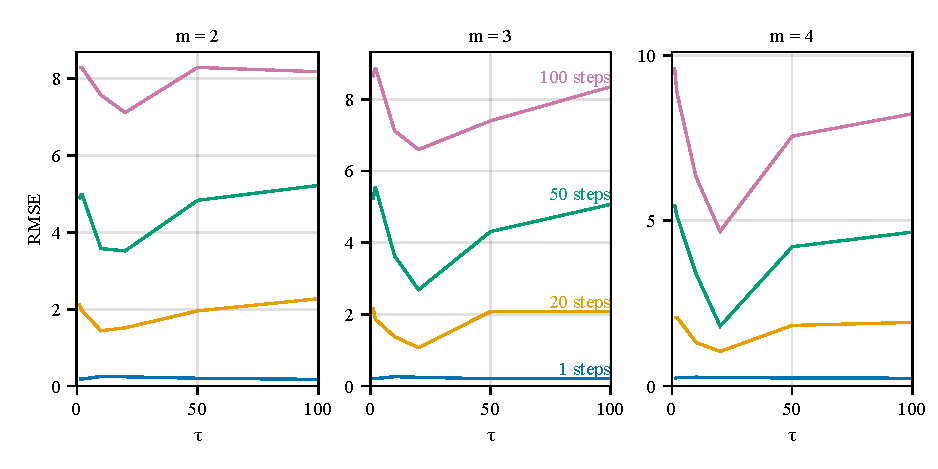
\includegraphics[width=1\textwidth]{../Images/ORSESN/ORSESN_tau_recursive_Lorenz 0_01.pdf}%[width=1.2\textwidth]
        }%[width=\textwidth,keepaspectratio]
        \caption{Iterative prediction RMSE for the ORSESN as a function of the partition delay $\tau$.}
        \label{fig:ORSESN_delay_iterative}
    \end{subfigure}

    \vspace{0em}

    \begin{subfigure}{\textwidth}
        \centering
        \makebox[\textwidth][c]{%
            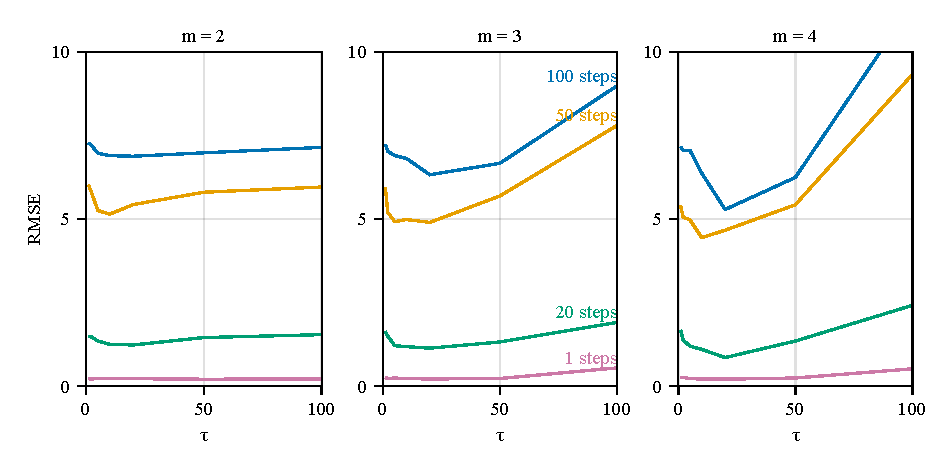
\includegraphics[width=1\textwidth]{../Images/ORSESN/ORSESN_tau_direct_Lorenz 0_01.pdf}%[width=1.2\textwidth]
        }%[width=\textwidth,keepaspectratio]
        \caption{Direct prediction RMSE for the ORSESN as a function of the partition delay $\tau$.}
        \label{fig:ORSESN_delay_direct}
    \end{subfigure}

    \caption{Prediction RMSE for the ORSESN as a function of the partition delay size $\tau$, with training data additive noise $\alpha=0.1$ and reservoir size $k=468$. Subfigures (a) and (b) correspond to iterative and direct prediction, respectively. Curves correspond to different numbers of prediction steps, and each axis represents an ORSESN with a different value for $m$.}
    \label{fig:ORSESN_delay_combined}
\end{figure}


\begin{table}
    \centering
    \begin{tabular}{lllccc}
        \toprule
        \textbf{Model} & \textbf{Dataset} & \textbf{Prediction Type} & \textbf{$m=2$} & \textbf{$m=3$} & \textbf{$m=4$} \\
        \midrule
        ORSESN & Lorenz 0.01 & Iterative & 20 & 20 & 20 \\
        ORSESN & Lorenz 0.05 & Iterative & 10 & 10 & 4 \\
        ORSESN & Rossler 0.1 & Iterative & 20 & 20 & 20 \\
        ORSESN & MG 0.5 & Iterative & 20 & 20 & 20 \\
        % ORSESN & MG 2.5 & Iterative & 50 & 50 & 50 \\
        \midrule
        ORSESN & Lorenz 0.01 & Direct & 20 & 20 & 20 \\
        ORSESN & Lorenz 0.05 & Direct & 4 & 4 & 4 \\
        ORSESN & Rossler 0.1 & Direct & 20 & 20 & 20 \\
        ORSESN & MG 0.5 & Direct & 20 & 20 & 20 \\
        % ORSESN & MG 2.5 & Direct & 50 & 50 & 20 \\
        \midrule % Separator between ORSESN and OPESN data
        OPESN & Lorenz 0.01 & Iterative & 20 & 20 & 20 \\
        OPESN & Lorenz 0.05 & Iterative & 10 & 10 & 4 \\
        OPESN & Rossler 0.1 & Iterative & 20 & 20 & 10 \\
        OPESN & MG 0.5 & Iterative & 20 & 20 & 20 \\
        % OPESN & MG 2.5 & Iterative & 50 & 50 & 50 \\
        \midrule
        OPESN & Lorenz 0.01 & Direct & 20 & 20 & 20 \\
        OPESN & Lorenz 0.05 & Direct & 4 & 4 & 4 \\
        OPESN & Rossler 0.1 & Direct & 10 & 20 & 10 \\
        OPESN & MG 0.5 & Direct & 20 & 20 & 20 \\
        % OPESN & MG 2.5 & Direct & 50 & 50 & 20 \\
        \bottomrule
    \end{tabular}
    \caption{Optimal partition delay values $\tau$ selected for ORSESN and OPESN models across different datasets and prediction types. Values are shown for each tested $m$ (ordinal pattern dimension), and were optimise to minimise RMSE.}
    \label{tab:taus}
\end{table}

\subsection{Practical considerations for the ordinal pattern dimension}

The number of possible partitions for a given value of $m$ is given by $m!$. Without additive noise the time series will visit a subset of these possible partitions, for example where $m=4$ the $x$ component of the simulated Lorenz system showed data points in 13 of the 24 possible partitions. Unsurprisingly however, with additive noise the time series will visit many more possible partitions, and for a sufficiently large noise level it will visit all possible partitions. For example where $m=4$ and with noise multipliers of $\alpha=[0.1, 0.2, 0.3]$ the $x$ component of the simulated Lorenz system showed data points in $[21, 22, 24]$ of the 24 possible partitions respectively.

For the architecture described in chapter \ref{chap:OPESNs}, the size of the reservoir is dependent on the number of expected partitions, calculated by $k_{total}=kN_{obs}$ where $N_{obs}$ is the number of observed partitions in the time series and $k$ is the desired number of nodes in each sub-reservoir. Varying the value $m$ for the same $k$ will thus produce a different total number of nodes $k_{total}$. ESNs have generally been found to produce a better prediction for a larger reservoir size~\cite{lukosevicius_and_jaeger_2009}~\cite{lukosevicius_2012_practical_guide}, so to compare between different values of $m$ we have chosen values of $k$ based on the number of observed partitions $N_{obs}$ for each time series and value of $m$ in order to produce comparable values of $k_{total}$. It is important to approximately match the total size of reservoirs to delineate the effect of dividing the reservoir into sub-reservoirs and the effect of increasing the total reservoir size. The reader should note that an OPESN with $m=5$ has up to $5!=120$ possible patterns. To allow each sub-reservoir of the OPESN to have at least $k=20$ nodes could require $k_{total} \geq 2000$, which is not feasible to test under our compute resource constraints.

For the architecture described in chapter \ref{chap:ORSESN}, the readout matrix will be of size $k \times N_{obs}$. For a reservoir of size $k=500$ and $m=5$, the readout matrix could be up to $500(5!)=60000$ parameters. An ESN reservoir with connection probability $0.05$ will have an expected number of non-zero parameters $\mathbb{E}[\|\mathbf{W}_{rec}\|_0] = 0.05(500^2) = 12500$. The reader can see that as we increase $m$, the ORSESN's readout size will scale factorially and that for $m>4$ the size of the ORSESN's readout will be far larger than the number of non-zero parameters of the reservoir, forming a degenerate kind of ESN. For this reason we have not tested the ORSESN model for $m>4$.

\subsection{Testing procedure}

To test each particular set of parameters we performed 30 trials, creating a new ESN each time. Creating a new ESN includes randomly instantiating the weights and the reservoir states, and fitting a new readout vector, ensuring that the trials are independent of one another. We aggregate the trials by finding the mean, standard deviation, minimum and maximum of the RMSE of their predictions~\cite{lukosevicius_2012_practical_guide}. We report means $\pm 1.96 \times$ standard error across the 30 trials; a mean outside the baseline CI is considered significant.

A multi-step prediction can extend to an arbitrary number of steps into future $(y_1,...,y_n)$ and these predictions could then be sub-sampled to a shorter number of prediction steps. Thus the same multistep prediction could yield error metrics for multiple different numbers of steps, but these metrics would not be independent. So for the purposes of our testing, we have regenerated the multistep predictions for each number of steps anew using a new ESN each time.

% !TEX root = ../HonoursThesis.tex

\renewcommand{\chapterlabel}{Chapter}
\chapter{Echo state network with ordinal partition based readout switching}
\label{chap:ORSESN}


The first approach uses a piecewise readout function to incorporate ordinal partition information into the structure of an ESN. In this architecture there is a different readout vector for each observed ordinal partition and at each time step, a readout vector is chosen depending on the partition of the input data. We will refer to this architecture as the Ordinal partition based Readout Switching ESN (ORSESN).

% \begin{figure}
%     \centering
%     \begin{tikzpicture}[scale=1.2]
%         \node[fill=col1,circle,inner sep=4pt,label=left:$\mathbf{x}(t)$] (input) at (0,0) {};
%         \node[fill=black,circle,inner sep=2pt,label=right:$\mathbf{y}(t)$] (output) at (10,0) {};
        
        
%         \coordinate (res_anchor) at (2,3);
%         \node[fill=black,circle,inner sep=2pt] (res1) at ({5-0.5},{0.8}) {};
%         \node[fill=black,circle,inner sep=2pt] (res2) at ({5},{-1}) {};
%         \node[fill=black,circle,inner sep=2pt] (res3) at ({5},{0.15}) {};
%         \node[fill=black,circle,inner sep=2pt] (res4) at ({5+1},{-0.1}) {};
%         \node[fill=black,circle,inner sep=2pt] (res5) at ({5-0.75},{-0.5}) {};
%         \node[fill=black,circle,inner sep=2pt] (res6) at ({5-1.25},{0.4}) {};
%         \node[fill=black,circle,inner sep=2pt] (res7) at ({5+0.65},{0.75}) {};
%         \node[fill=black,circle,inner sep=2pt] (res8) at ({5+1},{-0.9}) {};
%         \node[fill=black,circle,inner sep=2pt] (res9) at ({5-1.25},{-1}) {};
%         \node[fill=black,circle,inner sep=2pt] (res10) at ({5-1.75},{-0.25}) {};

%         \foreach \i in {1,...,10}
%             \draw[gray,line width=0.1] (input) -- (res\i);
        
%         \foreach \i in {1,...,5}
%             \foreach \j in {1,...,5} {
%                 \ifnum\i<\j
%                     \draw (res\i) -- (res\j);
%                 \fi
%             }
        
%         \draw (res6) -- (res5);
%         \draw (res6) -- (res1);
%         \draw (res6) -- (res10);
%         \draw (res10) -- (res5);
%         \draw (res9) -- (res10);
%         \draw (res9) -- (res2);
%         \draw (res7) -- (res1);
%         \draw (res7) -- (res3);
%         \draw (res7) -- (res4);
%         \draw (res8) -- (res4);
%         \draw (res8) -- (res2);
        
%         \foreach \i in {1,...,10}
%             \draw[gray,line width=0.1] (res\i) -- (output);
        
%         \begin{scope}[on background layer]
%         \draw[draw=black,fill=pale_yellow,rounded corners=8pt]  ($(res1)+(-0.1,0.3)$) -- ($(res7)+(+0.2,+0.2)$) -- ($(res4)+(0.4,0)$) -- ($(res8)+(0.2,-0.2)$) -- ($(res2)+(0,-0.2)$) -- ($(res9)+(-0.2,-0.2)$) -- ($(res10)+(-0.3,0)$) -- ($(res6)+(-0.3,0)$) -- cycle;
%         \end{scope}
%         \node at (5.2, 1.4) {$\mathbf{W}_{\text{rec}}$};
%         \node at (5, -1.6) {$\mathbf{s}(t)$};
        
%         \draw[fill=white,opacity=0.8] (1.2,-0.75) rectangle (2.0,0.75) node[midway] {$\mathbf{W}_{\text{in}}$};
%         % \draw[fill=col3,opacity=0.8] (8, -0.75+2) rectangle (8.8,0.75+2) node[midway, text=white] {$\mathbf{C}_{\text{out}}$};
%         \draw[fill=col1,opacity=0.8] (8, -0.75) rectangle (8.8,0.75) node[midway, text=white] {$\mathbf{C}_{\text{out}}$};
%         % \draw[fill=col2,opacity=0.8] (8, -0.75-2) rectangle (8.8,0.75-2) node[midway, text=white] {$\mathbf{C}_{\text{out}}$};
%     \end{tikzpicture}

%     \begin{tikzpicture}[scale=1.2]
%         \node[fill=col2,circle,inner sep=4pt,label=left:$\mathbf{x}(t)$] (input) at (0,0) {};
%         \node[fill=black,circle,inner sep=2pt,label=right:$\mathbf{y}(t)$] (output) at (10,0) {};
        
        
%         \coordinate (res_anchor) at (2,3);
%         \node[fill=black,circle,inner sep=2pt] (res1) at ({5-0.5},{0.8}) {};
%         \node[fill=black,circle,inner sep=2pt] (res2) at ({5},{-1}) {};
%         \node[fill=black,circle,inner sep=2pt] (res3) at ({5},{0.15}) {};
%         \node[fill=black,circle,inner sep=2pt] (res4) at ({5+1},{-0.1}) {};
%         \node[fill=black,circle,inner sep=2pt] (res5) at ({5-0.75},{-0.5}) {};
%         \node[fill=black,circle,inner sep=2pt] (res6) at ({5-1.25},{0.4}) {};
%         \node[fill=black,circle,inner sep=2pt] (res7) at ({5+0.65},{0.75}) {};
%         \node[fill=black,circle,inner sep=2pt] (res8) at ({5+1},{-0.9}) {};
%         \node[fill=black,circle,inner sep=2pt] (res9) at ({5-1.25},{-1}) {};
%         \node[fill=black,circle,inner sep=2pt] (res10) at ({5-1.75},{-0.25}) {};

%         \foreach \i in {1,...,10}
%             \draw[gray,line width=0.1] (input) -- (res\i);
        
%         \foreach \i in {1,...,5}
%             \foreach \j in {1,...,5} {
%                 \ifnum\i<\j
%                     \draw (res\i) -- (res\j);
%                 \fi
%             }
        
%         \draw (res6) -- (res5);
%         \draw (res6) -- (res1);
%         \draw (res6) -- (res10);
%         \draw (res10) -- (res5);
%         \draw (res9) -- (res10);
%         \draw (res9) -- (res2);
%         \draw (res7) -- (res1);
%         \draw (res7) -- (res3);
%         \draw (res7) -- (res4);
%         \draw (res8) -- (res4);
%         \draw (res8) -- (res2);
        
%         \foreach \i in {1,...,10}
%             \draw[gray,line width=0.1] (res\i) -- (output);
        
%         \begin{scope}[on background layer]
%         \draw[draw=black,fill=pale_yellow,rounded corners=8pt]  ($(res1)+(-0.1,0.3)$) -- ($(res7)+(+0.2,+0.2)$) -- ($(res4)+(0.4,0)$) -- ($(res8)+(0.2,-0.2)$) -- ($(res2)+(0,-0.2)$) -- ($(res9)+(-0.2,-0.2)$) -- ($(res10)+(-0.3,0)$) -- ($(res6)+(-0.3,0)$) -- cycle;
%         \end{scope}
%         \node at (5.2, 1.4) {$\mathbf{W}_{\text{rec}}$};
%         \node at (5, -1.6) {$\mathbf{s}(t)$};
        
%         \draw[fill=white,opacity=0.8] (1.2,-0.75) rectangle (2.0,0.75) node[midway] {$\mathbf{W}_{\text{in}}$};
%         \draw[fill=col2,opacity=0.8] (8, -0.75) rectangle (8.8,0.75) node[midway, text=white] {$\mathbf{C}_{\text{out}}$};
%     \end{tikzpicture}
%     % \caption{echo state network with readout switching.}
%     \caption{Architecture of the Ordinal partition based Readout Switching ESN (ORSESN). Input $\mathbf{x}(t)$ is projected into a reservoir of $k=10$ nodes via $\mathbf{W}_{\mathrm{in}}$ and recurrently updated via $\mathbf{W}_{\mathrm{rec}}$. Partition specific readout vectors $\mathbf{C}_{\mathrm{out}}$ are selected based on the active ordinal partition, illustrated by colours purple and orange.}
%     \label{fig:readout_switching_ESN}
% \end{figure}

% TODO discuss Ma \& Chen (2013) and their state space partitioning and compare it to this case.

\section{Implementation}

\subsection{Instantiating the weights and iterating the reservoir}

The input weights $\mathbf{W}_{in}$ and recurrence matrix $\mathbf{W}_{rec}$ of the ORSESN are generated as they would be for a traditional ESN. $\mathbf{W}_{in}$ is a vector of length $k$ drawn from a Normal distribution and $\mathbf{W}_{rec}$ is an Erd\H{o}s-R\'enyi random network adjacency matrix. The initial states $s(0)$ form a vector of length $k$ and are initialised by drawing from a Normal distribution. The ORSESN can be driven with the input and the reservoir iterated just like a traditional ESN, using the update equation:

\[
    \mathbf{s}(t + 1) = f_{act}(\mathbf{W}_{in}\mathbf{x}(t) + \mathbf{W}_{rec}\mathbf{s}(t) + \mathbf{W}_{bias}).
\]

Driving the reservoir with the training sequence and collecting the states into a matrix $\mathbf{S}$ will prepare us to fit the vectors that make up the piecewise readout function. For a training sequence of length $n_{train}$, let us collect these states into a matrix:
\[
    \mathbf{S} = [\mathbf{s}(1), ..., \mathbf{s}(n_{train})]^t \in R^{n_{train}\times k}.
\]

\subsection{Fitting the readout vectors}

To fit the readout vector for each partition $\pi$, we must filter the input time series $\mathbf{Y}$ to those data points belonging to that partition $\pi$ and filter the states $\mathbf{S}$ to those that arose immediately after that input from that partition $\pi$. We can define those inputs $\mathbf{Y}_\pi$ and states $\mathbf{S}_{\pi}$ that relate to each partition $\pi$ by indexing $\mathbf{Y}$ and $\mathbf{S}$, where $\pi_t$ represents the ordinal partition of the data at time $t$:
\begin{align*}
    \mathbf{Y}_\pi &= \{\mathbf{Y}_{t} | \pi_t = \pi\}, \\
    \mathbf{S}_\pi &= \{\mathbf{S}_{t,*} | \pi_t = \pi\},
\end{align*}
and then for each partition $\pi$, we can fit a readout vector using Ridge regression:
\[
    (\mathbf{C}_{out}^T)_\pi = (\mathbf{S}_\pi^T \mathbf{S}_\pi + \beta \mathbf{I}) \ \mathbf{S}_\pi^T \mathbf{Y}_\pi.
\]
The readout vectors for each partition can then be arranged into an $N_{obs}\times k$ matrix,
\[
    \mathbf{C}_{out} = [(\mathbf{C}_{out})_1; ...; (\mathbf{C}_{out})_{N_{obs}}],
\]
and a vector of predictions for each possible partition $\mathbf{y}_{all}(t)$ at time $t$ can be inferred for any states $\mathbf{s}(t)$:
\[
    \mathbf{y}_{all}(t) = \mathbf{C}_{out}(t)\mathbf{s}(t).
\]

To obtain just one of these predictions, we construct a mask based on the active partition at each time step. This mask $e_\pi$ will be a `one-hot encoded' vector of length $N_{obs}$, where 1 indicates the active partition at that time step and 0 indicates the other inactive partitions. By multiplying our mask and the prediction vector and summing the result, we can select the prediction for a given ordinal partition $\pi_t$:
\[
    \mathbf{y}(t) = \sum \mathbf{y}_{all}(t)e_{\pi_t}.
\]

The selection of the prediction does not necessarily need to be one-hot like this, but could use an informed combination of predictions, as do other mixture-of-experts models~\cite{babinec_pospichal_2009}~\cite{laan_vicente_2015}. One such relevant method could be to weight the predictions of each of the partition readouts depending on the transition probabilities of the active ordinal partition, however we have not trialed this hypothesis.

Here we have defined a method for `switching' the readout of an ESN based on the ordinal partition of the input data.%Figure \ref{fig:readout_switching_ESN} visualises the switching of just the readout vector using the colour coding of ordinal partitions introduced in chapter \ref{chap:ordinal_partitions}.




\section{Results}



\subsection{Lorenz - iterative prediction}

First we will consider the mean RMSE created by iterative predictions of the Lorenz time series with a $\Delta t = 0.01$. At a single recursive prediction step, the traditional ESN achieves the lowest mean RMSE of 0.173 ($\pm 0.025$), outperforming the ORSESN for all ordinal pattern dimensions ($m$). For $m=2$, $3$, and $4$, the mean RMSEs are 0.237 ($\pm 0.015$), 0.258 ($\pm 0.012$), and 0.268 ($\pm 0.010$), respectively. This shows that for short term predictions, increasing the ordinal pattern dimension $m$ leads to a higher mean RMSE for the ORSESN, and that the traditional ESN is optimal for very short-term predictions. However, as the number of recursive prediction steps increases, this relationship changes. After two and three steps, the RMSEs for all models increase, but the gap between the traditional ESN and the ORSESN with higher $m$ begins to narrow. For example, at 3 steps, the traditional ESN has a mean RMSE of 0.334 ($\pm 0.055$), while the ORSESN with $m=4$ has a mean RMSE of 0.341 ($\pm 0.034$).

The significant change occurs at longer prediction horizons, as shown in Figure \ref{fig:ORSESN_iterative_0_01}. By 10 steps, the traditional ESN's mean RMSE rises to 1.093 ($\pm 0.159$), while the ORSESN with $m=4$ achieves a significantly lower (95\% CI) mean RMSE of 0.739 ($\pm 0.086$).
At 20 steps, the error rates have reversed: the traditional ESN's RMSE increases to 2.072 ($\pm 0.230$), whereas the ORSESN achieves significantly lower (95\% CI) errors for all $m$, with $m=4$ reaching the lowest RMSE of 1.004 ($\pm 0.092$). This advantage becomes even more pronounced as the prediction horizon extends further, with the ORSESN with $m=4$ achieving a mean RMSE of approximately 3.174 ($\pm 0.254$) at 70 steps compared to the traditional ESN's 6.915 ($\pm 0.732$). However for $m=2$, the trend does not significantly hold, with the $m=2$ ORSESN's mean RMSE failing to be significantly lower for most prediction horizons. The $m=3$ ORSESN ceases to provide a significant benefit at 200 prediction steps, beyond which all four models diverge from the signal.
These results demonstrate that, although the traditional ESN is best for immediate predictions, the ORSESN with higher ordinal pattern dimension $m$ provides significantly more accurate and stable predictions for longer prediction horizons.

The ORSESN also demonstrates greater consistency in its predictions compared to the traditional ESN, as measured by the standard deviation of RMSE across trials. Since each trial uses a newly instantiated set of states and weights, and regenerates the additive noise for the time series, the standard deviation of the RMSEs generated by each trial can represent how robust each architecture is to its random initial conditions. The ORSESN achieves a lower standard deviation of RMSE across trials, especially at longer prediction horizons. At 10 recursive steps, the traditional ESN shows a standard deviation of 0.159, while the ORSESN with $m=4$ has a much lower value of 0.086. This pattern continues at 30 steps (0.511 vs. 0.116) and 50 steps (0.679 vs. 0.147). Notably, the variability decreases as the ordinal pattern dimension increases, with $m=4$ consistently showing the lowest standard deviations in the medium-term prediction range.

When examining the Lorenz system with a larger time step size of $\Delta t=0.05$, we observe similar patterns although less pronounced. The traditional ESN has a mean RMSE of 1.330 ($\pm 0.040$) at a single prediction step, which is comparable to the ORSESN with $m=3$ (1.337 $\pm 0.055$) and $m=4$ (1.328 $\pm 0.059$). Compared to the Lorenz series with $\Delta t=0.01$, the performance of the ORSESN improves over the traditional ESN at even shorter prediction lengths. After just 2 recursive prediction steps, the ORSESN with $m=4$ already demonstrates significantly (95\% CI) superior performance with a mean RMSE of 1.483 ($\pm 0.040$) compared to the traditional ESN's 1.535 ($\pm 0.017$). The ORSESN with $m=3$ demonstrates significantly superior performance at 20 time steps, and $m=2$ at 30, but by 70 prediction steps, all three models have converged, as shown in Figure \ref{fig:ORSESN_iterative_0_05}.
% For 20 recursive prediction steps and beyond, the ORSESN models also showed consistently lower standard deviations.


\begin{figure}
    \centering

    \begin{subfigure}{\textwidth}
        \caption{Mean iterative prediction RMSE on the Lorenz series with time step size $\Delta t = 0.01$ for the ORSESN with delay $\tau=20$, noise level $\alpha=0.1$, and total reservoir size $k=500$.}
        \label{fig:ORSESN_iterative_0_01}
        \centering
        \makebox[\textwidth][c]{%
            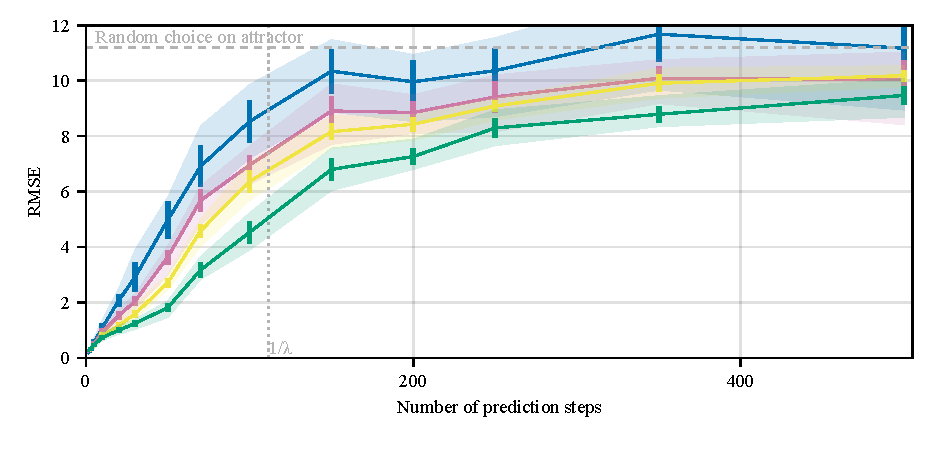
\includegraphics[width=1.1\textwidth,trim=0 8mm 0 0,clip]{../Images/ORSESN/ORSESN_topline_recursive_Lorenz 0_01.pdf}
        }
    \end{subfigure}

    \vspace{0.5em}

    \begin{subfigure}{\textwidth}
        \caption{Mean iterative prediction RMSE on the Lorenz series with time step size $\Delta t=0.05$ for the ORSESN with delays $\tau=10,10,4$ for $m=2,3,4$ respectively, noise level $\alpha=0.1$, and total reservoir size $k=500$.}
        \label{fig:ORSESN_iterative_0_05}
        \centering
        \makebox[\textwidth][c]{%
            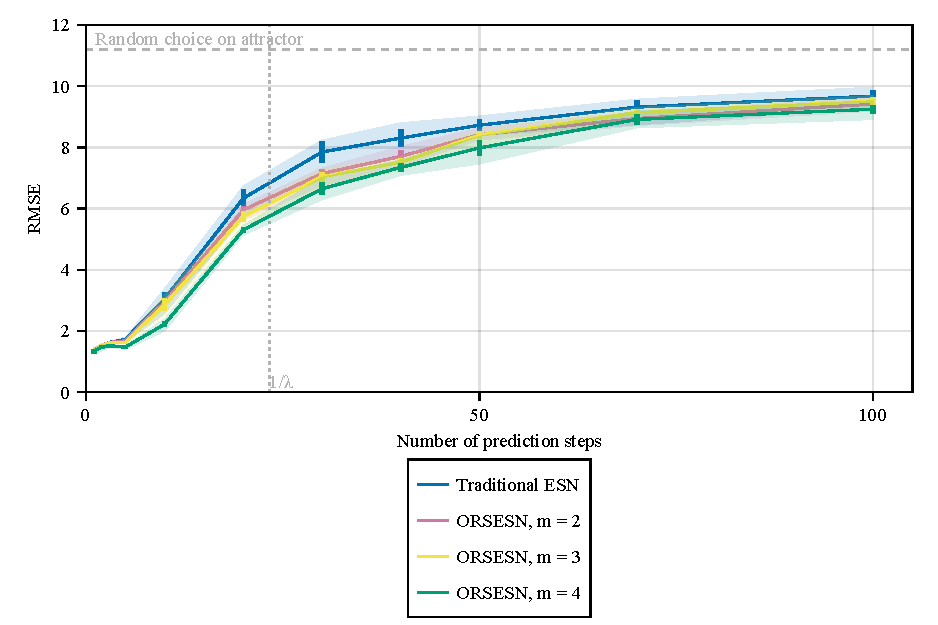
\includegraphics[width=1.1\textwidth]{../Images/ORSESN/ORSESN_topline_recursive_Lorenz 0_05.pdf}
        }
    \end{subfigure}

    % \caption{Mean iterative prediction RMSE for the ORSESN for Lorenz x component time series with two different time steps: (a) $\Delta t=0.01$ and (b) $\Delta t=0.05$, both with additive noise $\alpha=0.1$, delay $\tau=20$ and total reservoir size $k=468$. The standard deviations between trials are represented by vertical bars and the range of trial results is represented by the shaded regions.}
    \caption{Mean iterative prediction RMSE for the ORSESN on the Lorenz $x$-component time series with additive noise $\alpha=0.1$ and total reservoir size $k=500$. Subfigure (a) shows results for time step size $\Delta t=0.01$, delay $\tau=20$ for all $m$; subfigure (b) shows results for time step size $\Delta t=0.05$, delays $\tau=10,10,4$ for $m=2,3,4$, respectively. Standard deviations between trials are represented by vertical bars and shaded regions indicate the full range of trial results.}
\end{figure}



\subsection{Lorenz - direct prediction}


Here we will analyse the ability of the ORSESN to generate direct predictions. For the Lorenz system with time step size $\Delta t=0.01$, as shown in Figure \ref{fig:ORSESN_direct_0_01}, the traditional ESN initially performs well for short prediction horizons, achieving a mean RMSE of 0.228 ($\pm 0.033$) after 1 step. The ORSESN models show slightly higher errors at this prediction length, with mean RMSEs of 0.243 ($\pm 0.020$), 0.233 ($\pm 0.017$), and 0.228 ($\pm 0.021$) for $m=2$, $m=3$, and $m=4$, respectively. But mirroring what we observed in the iterative predictions, the ORSESN models perform better at longer prediction lengths. At 20 prediction steps, all three ORSESN models achieve a statistically significant (95\% CI) lower mean RMSE than the traditional ESN, with a higher $m$ producing a lower RMSE over the whole tested range of prediction lengths.

For direct prediction on the Lorenz system with time step size $\Delta t=0.05$ (Figure \ref{fig:ORSESN_direct_0_05}), the ORSESN with $m=4$ outperforms the traditional ESN from the start (mean RMSE of $0.239\pm 0.019$ vs. $0.311\pm 0.025$ at 1 step) and maintains this advantage throughout longer horizons ($0.759\pm 0.045$ vs. $1.175\pm 0.076$ at 5 steps; $5.003\pm 0.088$ vs. $6.214\pm 0.254$ at 20 steps). The ORSESN with $m=3$ also reliably outperforms the traditional ESN, however the ORSESN with $m=2$ fails to significantly improve (95\% CI) the traditional ESN at many prediction lengths.

Both direct and iterative prediction methods confirm the same conclusion: while traditional ESNs are superior or on-par for short-term forecasts, the ORSESN provides more accurate and stable predictions for medium to long-term horizons, with performance improving as the ordinal pattern dimension increases. The direct prediction results further confirm that the ORSESN's superior performance is not an artifact of error accumulation in iterative prediction but rather reflects a genuine improvement in the model's ability to capture the underlying dynamics of the chaotic system. There is a consistent pattern of lower errors for the ORSESN at longer prediction horizons across both forms of prediction.


\begin{figure}
    \centering

    \begin{subfigure}{\textwidth}
        \caption{Mean direct prediction RMSE on the Lorenz series with time step size $\Delta t=0.01$ for the ORSESN with delay $\tau=20$, noise level $\alpha=0.1$, and total reservoir size $k=500$.}
        \label{fig:ORSESN_direct_0_01}
        \centering
        \makebox[\textwidth][c]{%
            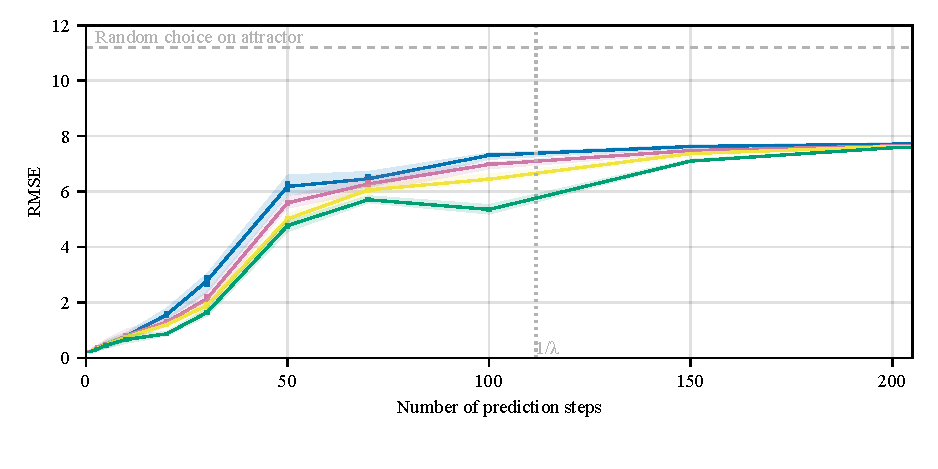
\includegraphics[width=1.1\textwidth,trim=0 8mm 0 0,clip]{../Images/ORSESN/ORSESN_topline_direct_Lorenz 0_01.pdf}
        }
    \end{subfigure}

    \vspace{0.5em}

    \begin{subfigure}{\textwidth}
        \caption{Mean direct prediction RMSE on the Lorenz series with time step size $\Delta t=0.05$ for the ORSESN with delay $\tau=4$, noise level $\alpha=0.1$, and total reservoir size $k=500$.}
        \label{fig:ORSESN_direct_0_05}
        \centering
        \makebox[\textwidth][c]{%
            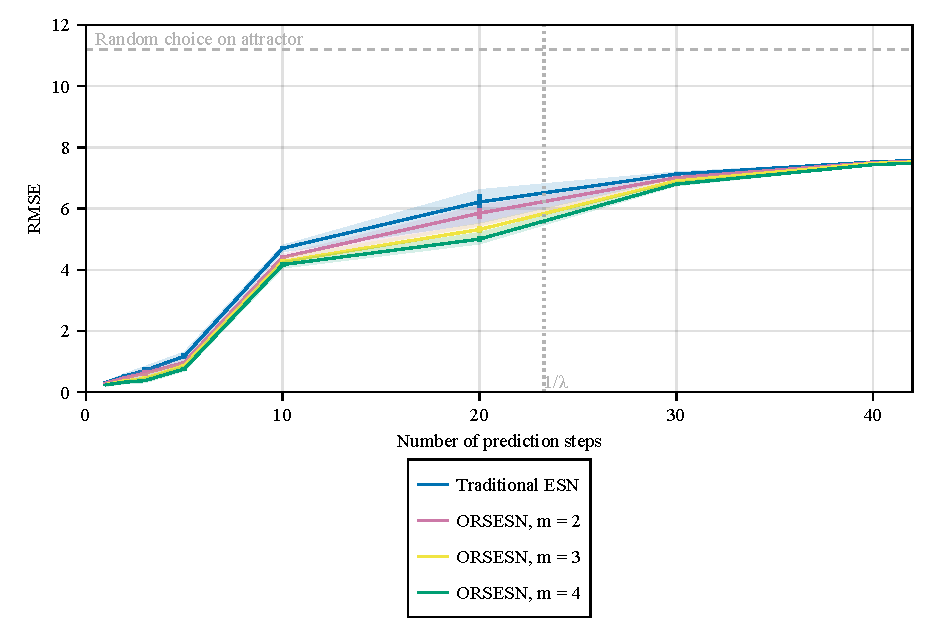
\includegraphics[width=1.1\textwidth]{../Images/ORSESN/ORSESN_topline_direct_Lorenz 0_05.pdf}
        }
    \end{subfigure}

    \caption{Mean direct prediction RMSE for the ORSESN on the Lorenz $x$-component time series with additive noise $\alpha=0.1$ and total reservoir size $k=500$. Subfigure (a) shows results for time step size $\Delta t=0.01$, delay $\tau=20$ for all $m$; subfigure (b) shows results for time step size $\Delta t=0.05$, delay $\tau=4$ for all $m$. Standard deviations between trials are represented by vertical bars and shaded regions indicate the full range of trial results.}
    \label{fig:ORSESN_direct}
\end{figure}



\subsection{Comparison across attractors}

\subsubsection{R\"ossler system}

For the R\"ossler system integrated with a time step size of $\Delta t=0.1$ (Figure~\ref{fig:ORSESN_rossler_iterative}), the results show a similar pattern to the Lorenz attractor. The traditional ESN exhibits lower error for very short term predictions, but after 5 recursive steps the mean RMSE of the ORSESN with $m=4$ ($0.374 \pm 0.0190$) and $m=3$ ($0.385 \pm 0.022$) significantly (95\% CI) outperform the traditional ESN ($0.482 \pm 0.041$). Like those predictions for the Lorenz series, this advantage becomes more pronounced at longer horizons; for instance, at 200 steps, ORSESN with $m=4$ achieves a significantly lower mean RMSE of 2.176 ($\pm 0.250$) compared to 4.393 ($\pm 1.126$) for the traditional ESN. Furthermore, the ORSESN with $m=4$ demonstrates remarkable prediction stability at this horizon, with a standard deviation of only 0.250, whereas the traditional ESN has a standard deviation of 1.126.

The ORSESN with $m=2$ fails to be significantly more accurate at multiple prediction lengths, and the ORSESN with $m=3$ provides insignificant improvement after 150 prediction steps. After 200 prediction steps, the ORSESN with $m=4$ no longer significantly outperforms the traditional ESN, but this can be seen to be a result of the higher standard deviation in the results of the traditional ESN.

Comparing these findings with the Lorenz system, the general performance characteristics are consistent. Traditional ESNs tend to be more accurate for shorter prediction lengths, however ORSESN models outperform on accuracy and stability for longer predictions lengths, particularly where $m=4$.
The crossover point, where ORSESN models begin to outperform traditional ESNs, typically occurs within the first 10 prediction steps for both chaotic systems.

What appears peculiar is the comparably low mean RMSE and small variance of the ORSESN with $m=4$. Figure \ref{fig:ORSESN_rossler_freerun} shows iterative predictions over 200 prediction steps (Rossler with $\Delta t = 0.1$) for the ORSESN and traditional ESN. Simply inspecting these predictions, all four models appear to predict the dynamics of only approximately one cycle before reverting to an `average' periodic prediction. However the ORSESN with $m=4$ appears to be able to predict the dynamics of 2 to 3 cycles to varying degrees of success before reverting to the `average' periodic prediction.



\begin{figure}
    \centering

    \centering
    \makebox[\textwidth][c]{%
        \includegraphics[width=1.1\textwidth,trim=0 0 0 0,clip]{../Images/ORSESN/ORSESN_topline_recursive_rossler 0_1.pdf}
    }

    \caption{Mean iterative prediction RMSE for the ORSESN for R\"ossler $x$ component time series with time step size $\Delta t=0.1$ and additive noise $\alpha=0.1$, delay $\tau=20$ and total reservoir size $k=500$. The standard deviations between trials are represented by vertical bars and the range of trial results is represented by the shaded regions.}
    \label{fig:ORSESN_rossler_iterative}
\end{figure}

\begin{figure}
    \centering
    \makebox[\textwidth][c]{%
        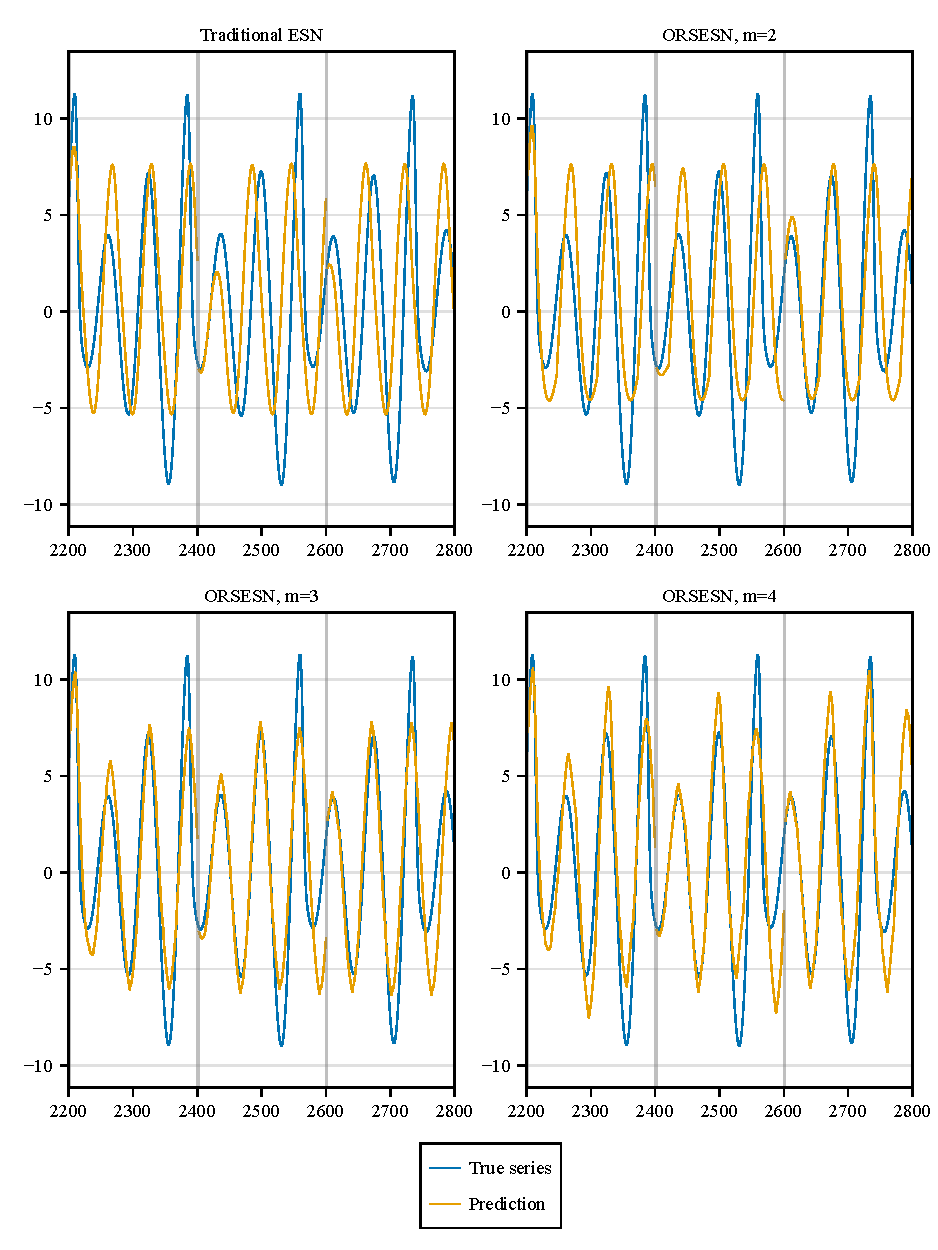
\includegraphics[width=1\textwidth,trim=0 0 0 0,clip]{../Images/ORSESN/ORSESN_freerun_recursive_Rossler.pdf}
    }
    \caption{Iterative free-run predictions for the Rössler system ($x$ component) with time step size $\Delta t=0.1$. The figure compares the traditional ESN with ORSESN models of varying ordinal pattern dimensions ($m=2,3,4$) over 200 prediction steps. All models were configured with a delay $\tau=20$, additive noise $\alpha=0.1$, and a total reservoir size $k=500$. Each grey vertical line indicates the beginning of prediction chunk, where the echo state network changes from being driven by the true signal to being driven by its own predictions.}
    \label{fig:ORSESN_rossler_freerun}
\end{figure}



The direct prediction performance on the Rössler system (Figure \ref{fig:ORSESN_rossler_direct}) is consistent with the iterative prediction trends. The benefit of the ORSESN appears more pronounced for the Rossler time series than the Lorenz time series.
Direct predictions on the Rossler series again shows the traditional ESN with slightly lower error for short predictions but the ORSESN models with higher ordinal pattern dimensions ($m$) generally achieve better accuracy for longer predictions. At 20 prediction steps, ORSESN with $m=4$ (mean RMSE $0.701\pm 0.058$) is significantly (95\%CI) more accurate than the traditional ESN (mean RMSE $1.094\pm 0.155$).
The mean prediction RMSE for all models converges, similar to the direct predictions for the Lorenz series, at approximately 350 prediction steps.
% A prediction at this length simply reflects the ESN's ability to match the periodicity of the data rather than its ability to represent the dynamics of the attractor.


\begin{figure}

    \centering
    \makebox[\textwidth][c]{%
        \includegraphics[width=1.1\textwidth,trim=0 0 0 0,clip]{../Images/ORSESN/ORSESN_topline_direct_rossler 0_1.pdf}
    }

    \caption{Mean direct prediction RMSE for the ORSESN for R\"ossler $x$ component time series with time step size $\Delta t=0.1$ and additive noise $\alpha=0.1$, delay $\tau=20$ and total reservoir size $k=500$. The standard deviations between trials are represented by vertical bars and the range of trial results is represented by the shaded regions.}
    \label{fig:ORSESN_rossler_direct}
\end{figure}



\subsubsection{Mackey-Glass system}

% apple
The iterative prediction results for the Mackey-Glass system with a time step size $\Delta t=0.5$ are illustrated in Figure \ref{fig:ORSESN_mg_iterative}.
Like the Lorenz and R\"ossler attractors, the traditional ESN demonstrates a clear advantage in single time step prediction for this system.

Similarly again, the ORSESN models generally show significantly (95\% CI) improved performance over the traditional ESN as the prediction horizon grows. For instance, at 20 recursive prediction steps, the traditional ESN has a mean RMSE of 0.110 ($\pm 0.010$), while the ORSESN with $m=2$ achieves 0.071 ($\pm 0.003$), $m=3$: 0.070 ($\pm 0.003$), and $m=4$: 0.039 ($\pm 0.001$).

Unlike the other attractors, the ORSESN models with $m=2$ and $m=3$ maintain significantly (95\% CI) improved accuracy only up to around 70 prediction steps, while the ORSESN with $m=4$ continues to provide improved accuracy for much longer predictions.

The ORSESN with $m=4$ achieves a consistent significantly (95\% CI) improved accuracy for all tested prediction lengths 5 time steps or longer. It maintains a much lower mean RMSE and a smaller standard deviation compared to both the traditional ESN and the other ORSESN configurations ($m=2,3$) for longer prediction horizons. For example, the performance at 100 steps is 62\% lower in error than the traditional ESN at 100 steps, with standard deviation of 0.002 much lower than the traditional ESN's 0.017. An example of the prediction of all four models can be found in Figure \ref{fig:ORSESN_mg_freerun}, however unlike the Rossler system, a simple qualitative explanation for the outperforming ORSESN with $m=4$ is not apparent.

\begin{figure}
    \centering

    % \begin{subfigure}{\textwidth}
        % \caption{Mean iterative prediction RMSE on the Mackey-Glass series with time step $\Delta t=0.5$ for the ORSESN with delay $\tau=20$.}
        % \label{fig:ORSESN_mg_iterative_0_5}
        % \centering
        \makebox[\textwidth][c]{%
            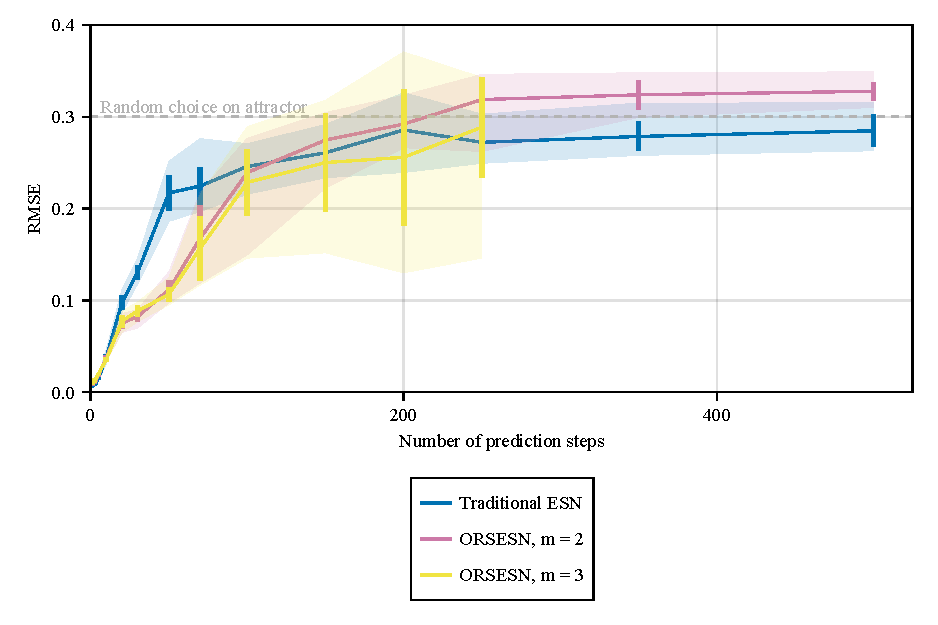
\includegraphics[width=1.1\textwidth,trim=0 0 0 0,clip]{../Images/ORSESN/ORSESN_topline_recursive_MG 0_5.pdf}
        }
    % \end{subfigure}

    % \vspace{0.5em}

    % \begin{subfigure}{\textwidth}
    %     \caption{TODO MORE TRIALS AND LONGER TEST SERIES Mean iterative prediction RMSE on the Mackey-Glass series with time step $\Delta t=2.5$ for the ORSESN with delay $\tau=50$.}
    %     \label{fig:ORSESN_mg_iterative_2_5}
    %     \centering
    %     \makebox[\textwidth][c]{%
    %         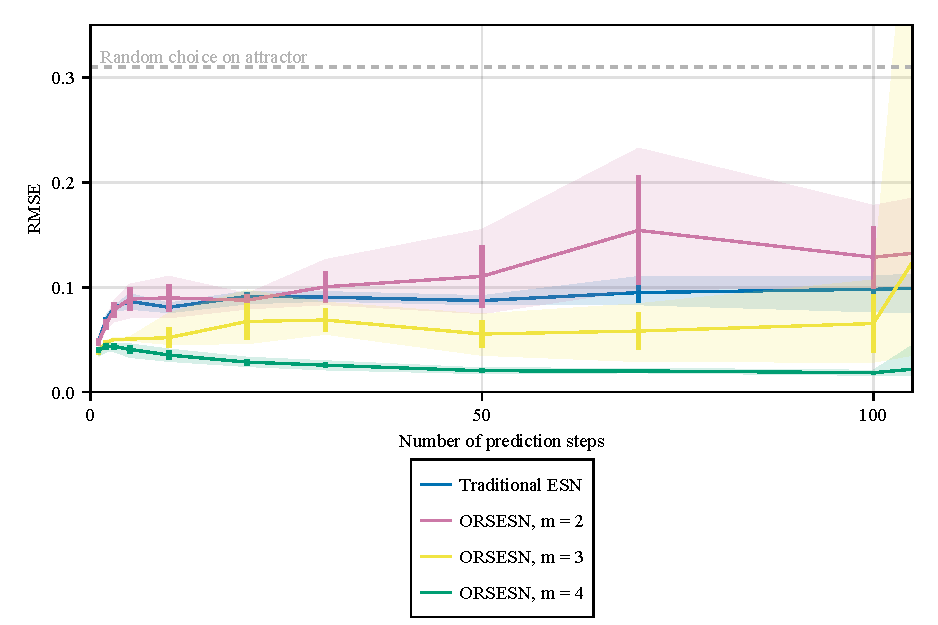
\includegraphics[width=1.1\textwidth]{../Images/ORSESN/ORSESN_topline_recursive_MG 2_5.pdf}
    %     }
    % \end{subfigure}

    % \caption{Iterative prediction RMSE for the ORSESN for Mackey-Glass time series with two different time steps: (a) $\Delta t=0.5$ (delay $\tau=20$) and (b) $\Delta t=2.5$ (delay $\tau=50$), both with additive noise $\alpha=0.1$ and total reservoir size $k=468$. The standard deviations between trials are represented by vertical bars and the range of trial results is represented by the shaded regions.}
    \caption{Iterative prediction RMSE for the ORSESN for Mackey-Glass time series with $\Delta t=0.5$, delay $\tau=20$, additive noise $\alpha=0.1$ and total reservoir size $k=500$. The standard deviations between trials are represented by vertical bars and the range of trial results is represented by the shaded regions.}
    \label{fig:ORSESN_mg_iterative}
\end{figure}

\begin{figure}
    \centering
    \makebox[\textwidth][c]{%
        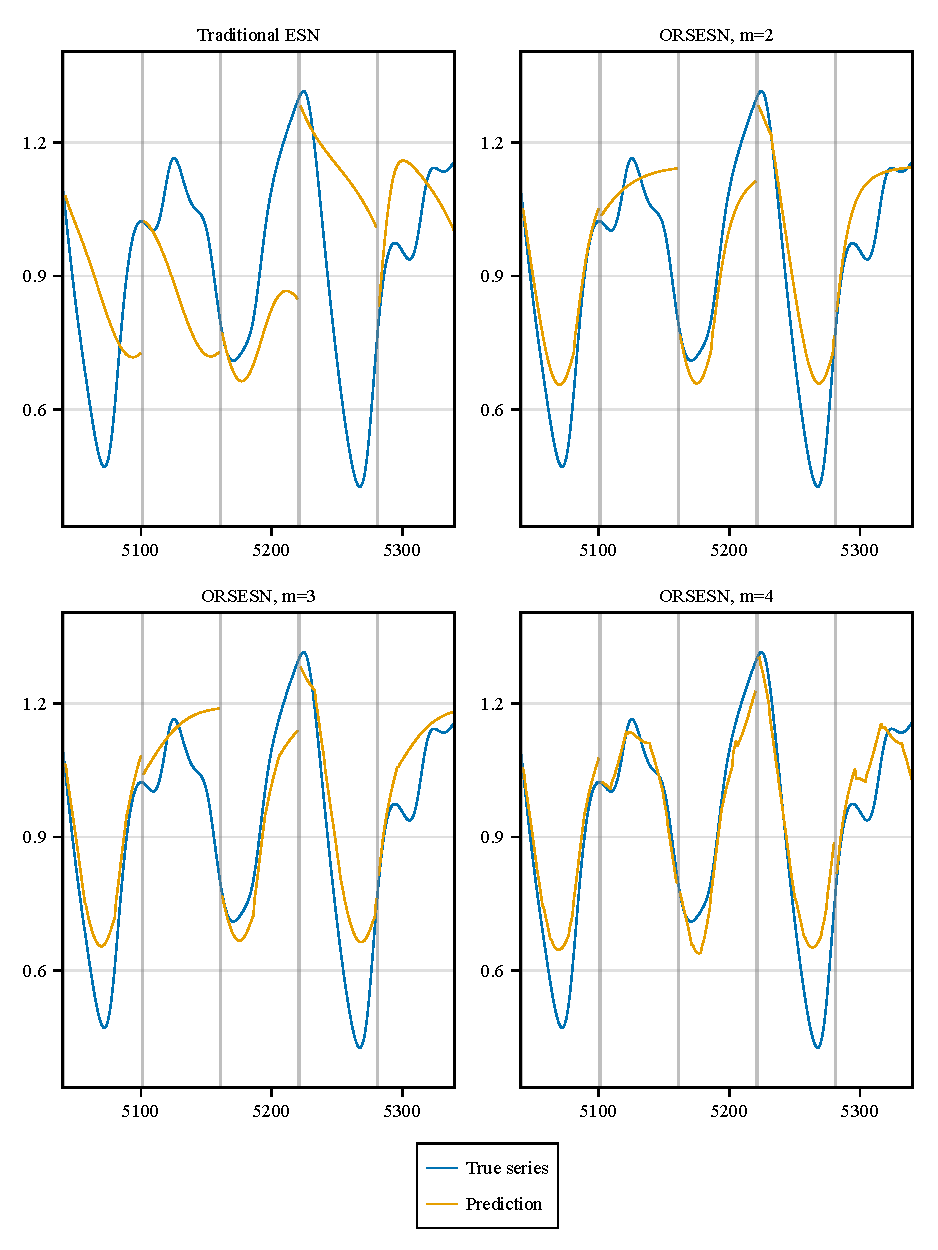
\includegraphics[width=1\textwidth]{../Images/ORSESN/ORSESN_freerun_recursive_Mackey_Glass.pdf}%
    }
    \caption{Example of iterative prediction for the Mackey-Glass system ($\Delta t=0.5$, additive noise $\alpha=0.1$). Predictions from the traditional ESN ($m=1, \tau=1$) and ORSESN ($m \in \{2,3,4\}, \tau=20$) are compared against the true series. All models use a total reservoir size $k=500$. Each grey vertical line indicates the beginning of prediction chunk, where the echo state network changes from being driven by the true signal to being driven by its own predictions.}
    \label{fig:ORSESN_mg_freerun}
\end{figure}

% apple
The direct prediction results for the Mackey-Glass system (Figure \ref{fig:ORSESN_mg_direct}) show a clear and consistent trend: the ORSESN produces a consistently lower mean RMSE, with $m=4$ achieving a significantly (95\%CI) superior result across all tested prediction lengths. This contrasts with the iterative prediction setting, where the advantage of higher $m$ is limited to shorter horizons and can degrade at longer ones; direct prediction has no crossover or degradation of performance for $m=2$ or $m=3$ at longer steps.

These results suggest that while the ORSESN with $m=2$ and $m=3$ can initially outperform the traditional ESN for medium length iterative predictions, they may be less effective at correcting for accumulating errors as the prediction length grows. This behavior leads to a crossover where the traditional ESN eventually matches or surpasses their performance.

However, this limitation is mitigated when the ordinal pattern dimension is increased to $m=4$. The ORSESN with $m=4$ not only maintains its initial advantage but also demonstrates sustained accuracy and stability across all tested prediction horizons. The mean RMSE for the $m=4$ ORSESN is 66\% lower than the traditional ESN at 10 direct prediction steps, and 51\% lower at 100 direct prediction steps. This indicates that a higher ordinal pattern dimension enables the ORSESN to capture more relevant dynamical information, resulting in both improved short term accuracy and greater resilience to error accumulation in long term predictions.




\begin{figure}
    \centering

    % \begin{subfigure}{\textwidth}
    %     \caption{Mean direct prediction RMSE on the Mackey-Glass series with time step $\Delta t=0.5$ for the ORSESN with delay $\tau=20$.}
    %     \label{fig:ORSESN_mg_direct_0_5}
    %     \centering
        \makebox[\textwidth][c]{%
            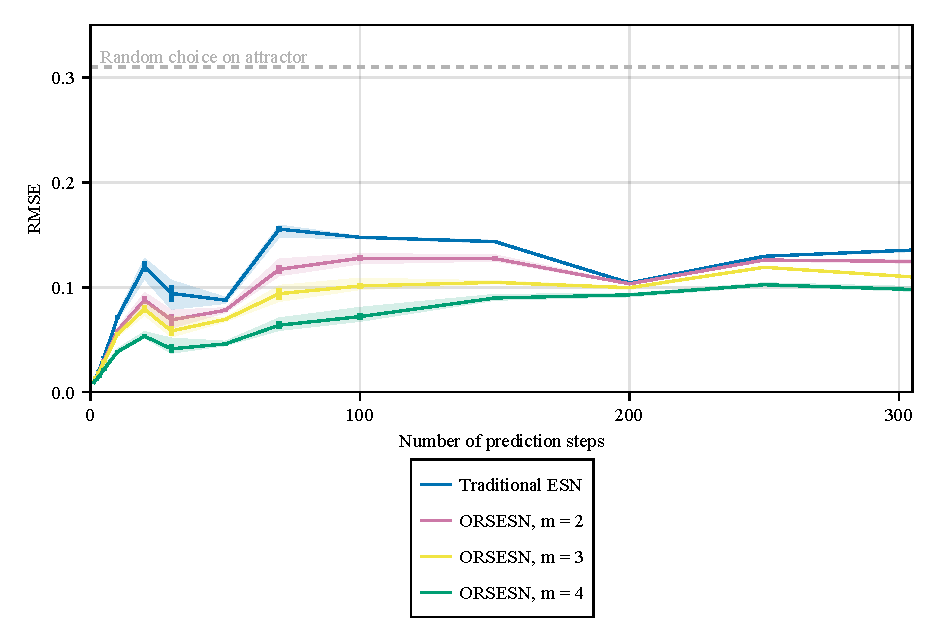
\includegraphics[width=1.1\textwidth]{../Images/ORSESN/ORSESN_topline_direct_MG 0_5.pdf}
        }
    % \end{subfigure}

    % \vspace{0.5em}

    % \begin{subfigure}{\textwidth}
    %     \caption{TODO MORE TRIALS AND LONGER TEST SERIES Mean direct prediction RMSE on the Mackey-Glass series with time step $\Delta t=2.5$ for the ORSESN with delays $\tau=50,50,20$ for $m=2,3,4$ respectively.}
    %     \label{fig:ORSESN_mg_direct_2_5}
    %     \centering
    %     \makebox[\textwidth][c]{%
    %         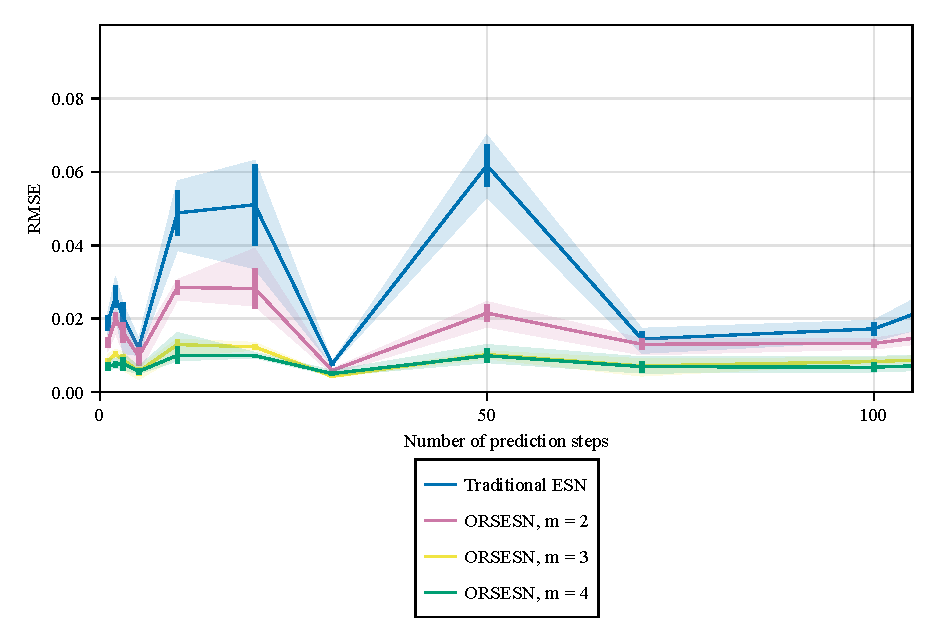
\includegraphics[width=1.1\textwidth]{../Images/ORSESN/ORSESN_topline_direct_MG 2_5.pdf}
    %     }
    % \end{subfigure}

    % \caption{Mean direct prediction RMSE for the ORSESN for Mackey-Glass time series with two different time steps: (a) $\Delta t=0.5$ (delay $\tau=20$) and (b) $\Delta t=2.5$ (delay $\tau=50$), both with additive noise $\alpha=0.1$ and total reservoir size $k=468$. The standard deviations between trials are represented by vertical bars and the range of trial results is represented by the shaded regions.}
    \caption{Mean direct prediction RMSE for the ORSESN for Mackey-Glass time series with $\Delta t=0.5$, delay $\tau=20$, additive noise $\alpha=0.1$ and total reservoir size $k=500$. The standard deviations between trials are represented by vertical bars and the range of trial results is represented by the shaded regions.}
    \label{fig:ORSESN_mg_direct}
\end{figure}





\subsection{Gating}


The ORSESN introduces a new architectural feature, the readout gating mechanism, and drives the gating using ordinal partition information of the incoming data. We would like to confirm whether it is the ordinal partition information that is creating the improved predictions rather than just the gating mechanism itself. To test this, we supplied the ORSESN with the Lorenz time series with $\Delta t=0.01$ accompanied by a random selection of the readout and compared it to the readout selection driven by the ordinal partition. Figure \ref{fig:ORSESN_routing_ordinal_vs_random} shows the performance of the ORSESN when its readout is gated via the ordinal partitions of the data compared to its performance when the gating of the readout is determined by random selection, for each of $m=2,3,4$. The performance of the ORSESN with random gating is insignificantly (95\% CI) different from the performance of our traditional ESN benchmark, with the mean RMSE value across trials lying within one standard deviation of the traditional ESN across all tested lengths of iterative prediction. We can infer from this testing that the predictive advantage of the ORSESN is likely conferred by the ordinal partition information rather than the use of the multiple readout vector gating mechanism by itself.

\begin{figure}
    \centering

    \begin{subfigure}{\textwidth}
        \caption{ORSESN Readout Gating - Ordinal Partition Driven vs. Random Selection, $m=2$}
        \label{fig:ORSESN_routing_m_2}
        \centering
        \makebox[\textwidth][c]{%
            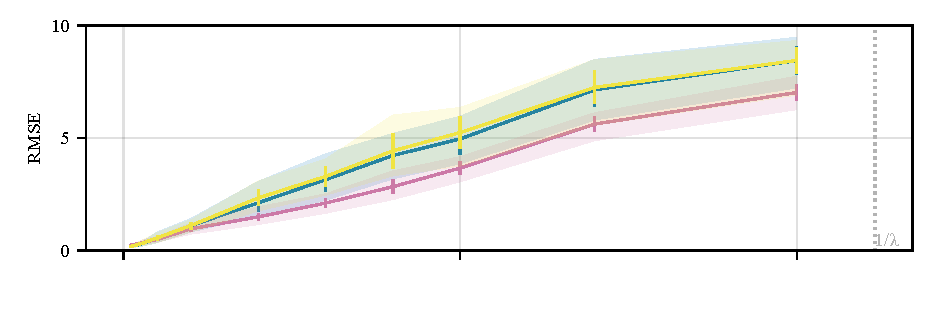
\includegraphics[width=1.1\textwidth,trim=0 0 0 3mm,clip]{../Images/ORSESN/ORSESN_routing_ordinal_vs_random_m=2.pdf}%
        }
    \end{subfigure}

    \vspace{0em}

    \begin{subfigure}{\textwidth}
        \caption{ORSESN Readout Gating - Ordinal Partition Driven vs. Random Selection, $m=3$}
        \label{fig:ORSESN_routing_m_3}
        \centering
        \makebox[\textwidth][c]{%
            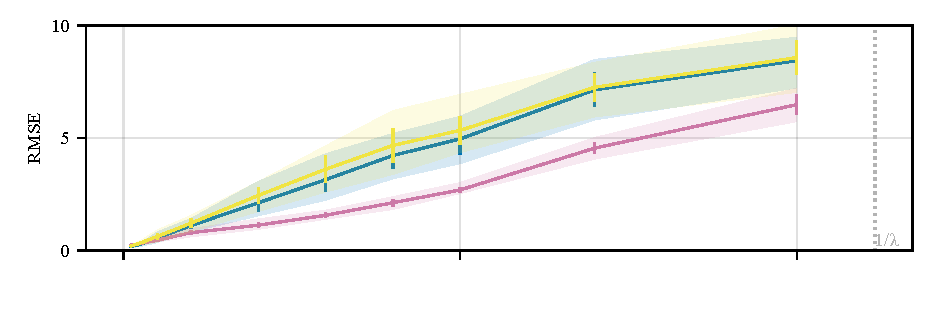
\includegraphics[width=1.1\textwidth,trim=0 0 0 3mm,clip]{../Images/ORSESN/ORSESN_routing_ordinal_vs_random_m=3.pdf}%
        }
    \end{subfigure}

    \vspace{0em}

    \begin{subfigure}[t]{\textwidth}
        \caption{ORSESN Readout Gating - Ordinal Partition Driven vs. Random Selection, $m=4$}
        \label{fig:ORSESN_routing_m_4}
        \centering
        \makebox[\textwidth][c]{%
            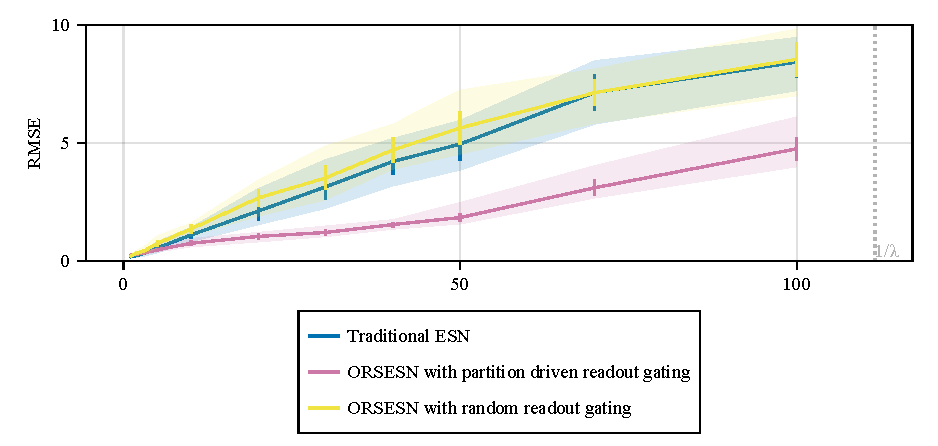
\includegraphics[width=1.1\textwidth,trim=0 0 0 3mm,clip]{../Images/ORSESN/ORSESN_routing_ordinal_vs_random_m=4.pdf}%
        }
    \end{subfigure}

    % \caption{Mean iterative prediction RMSE across trials for the ORSESN compared with a variant that chooses the readout randomly rather than dependent on the ordinal partition of the input, for delay $\tau=20$, noise level $\alpha=0.1$, and total reservoir size $k=468$. Subfigures (a), (b), and (c) correspond to $m=2$, $m=3$, and $m=4$, respectively. The standard deviations between trials are represented by vertical bars and the range of trial results is represented by the shaded regions.}
    \caption{Mean iterative prediction RMSE across trials for the ORSESN on the Lorenz $x$-component time series with time step size $\Delta t=0.01$, delay $\tau=20$, additive noise $\alpha=0.1$, and total reservoir size $k=468$, compared to a variant that selects the readout randomly rather than by ordinal partition. Subfigures (a), (b), and (c) correspond to $m=2$, $m=3$, and $m=4$, respectively. Standard deviations between trials are represented by vertical bars and shaded regions indicate the full range of trial results.}
    \label{fig:ORSESN_routing_ordinal_vs_random}
\end{figure}



\subsection{Resilience to noise}

We can test the resilience of models to noise by adding increasing levels of noise to the training data and testing the resulting prediction performance. We can then compare the effect of noise on the model's ability to create predictions. Figure \ref{fig:ORSESN_noise_resilience_direct} shows the mean direct prediction RMSE of multiple trials across values of noise $\alpha\in[0.0, 1.0]$, with four curves representing different numbers of prediction steps. As to be expected, as the level of noise increases so does the prediction RMSE for both the traditional ESN ($m=1$) and the ORSESN models ($m=2,3,4$). Compared to the traditional ESN, the ORSESN models appear to be less resilient to noise as the relative increase in RMSE is greater over noise levels $0.0$ to $1.0$. However the absolute mean RMSE is still lower (or approximately equal) for all $\alpha \in [0.0, 1.0]$ despite this lesser resilience to noise.

\begin{figure}
    \centering
    % ensure the graphic is centered and scaled to the text width without overflow
    \makebox[\textwidth][c]{%
        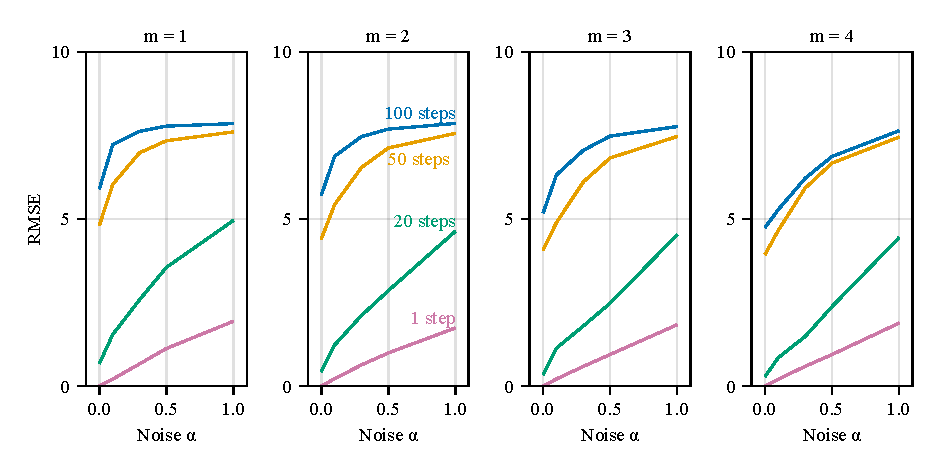
\includegraphics[width=1.1\textwidth]{../Images/ORSESN/ORSESN_direct_noise_resilience.pdf}%[width=1.2\textwidth]
    }%[width=\textwidth,keepaspectratio]
    % \caption{Mean direct prediction RMSE across trials for the OPESN as a function of simulated data noise level $\alpha$, with delay $\tau=20$ and reservoir size $k=468$. Curves correspond to different numbers of prediction steps, and each axis represents an ORSESN with a different value for $m$. The axis labeled $m=1$ refers to the traditional ESN.}
    \caption{Mean direct prediction RMSE across trials for the ORSESN on the Lorenz $x$-component time series with time step size $\Delta t=0.01$ as a function of simulated data noise level $\alpha$, with delay $\tau=20$ and total reservoir size $k=468$. Curves correspond to different numbers of prediction steps, and each panel represents an ordinal pattern dimension $m$ (with $m=1$ denoting the traditional ESN).}
    \label{fig:ORSESN_noise_resilience_direct}
\end{figure}

Figure \ref{fig:ORSESN_noise_resilience_iterative} shows the same noise analysis performed with iterative prediction instead of direct prediction. Iterative prediction yields similar results, where the traditional ESN appears to be more resilient to noise however the ORSESN has a lower (or approximately the same) mean prediction RMSE for $0.0 \leq \alpha \leq 1.0$. The reader can see that as the noise level increases, the predictive performance initially improves between $\alpha = 0.0$ and $\alpha = 0.1$ before degrading between $\alpha = 0.1$ and $\alpha = 1.0$. This `sweet spot' has been observed previously, where a modest amount of noise in training data lowers the prediction error of an ESN when producing iterative predictions~\cite{jaeger_2001}\cite{lukosevicius_and_jaeger_2009}. The benefit has been interpreted as a `mild stochastic regularisation', broadening the set of states seen during training so that the readout is less likely to compound small errors during iterative prediction. For the purposes of testing the performance of the traditional ESN and the ORSESN we have chosen the `sweet spot' value of $\alpha = 0.1$.

\begin{figure}
    \centering
    % ensure the graphic is centered and scaled to the text width without overflow
    \makebox[\textwidth][c]{%
        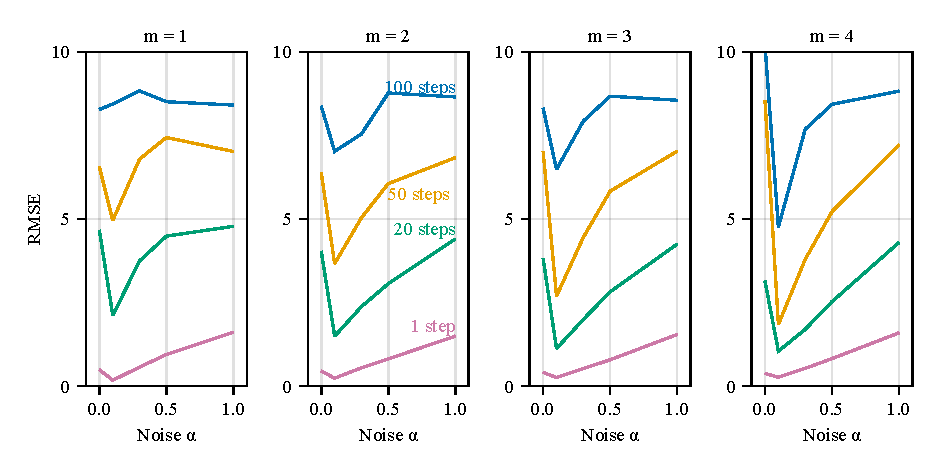
\includegraphics[width=1.1\textwidth]{../Images/ORSESN/ORSESN_recursive_noise_resilience.pdf}%[width=1.2\textwidth]
    }%[width=\textwidth,keepaspectratio]
    % \caption{Iterative prediction RMSE for the ORSESN as a function of simulated data noise level $\alpha$, with delay $\tau=20$ and reservoir size $k=468$. Curves correspond to different numbers of prediction steps, and each axis represents an ORSESN with a different value for $m$. The axis labeled $m=1$ refers to the traditional ESN.}
    \caption{Mean iterative prediction RMSE across trials for the ORSESN on the Lorenz $x$-component time series with time step size $\Delta t=0.01$ as a function of simulated data noise level $\alpha$, with delay $\tau=20$ and total reservoir size $k=468$. Curves correspond to different numbers of prediction steps, and each panel represents an ordinal pattern dimension $m$ (with $m=1$ denoting the traditional ESN).}
    \label{fig:ORSESN_noise_resilience_iterative}
\end{figure}

In an effort to explain this result, one should note that ordinal partitions are invariant to monotonic transformations but they are not immune to misclassification when the signal is noisy. Figures \ref{fig:ORSESN_noise_resilience_direct} and \ref{fig:ORSESN_noise_resilience_iterative} show that prediction error grows faster with $\alpha$ for ORSESN than for the traditional ESN, because additive noise can flip the relative order of nearby samples and therefore trigger an incorrect readout. In other words, as we increase $\alpha$ we are pushing the gating mechanism to become random - the effects of which have been tested above. Nevertheless ORSESN preserves an absolute advantage up to $\alpha=1.0$ in the present setting, implying that its gains outweigh the extra sensitivity unless measurement noise is extreme. For applications where noise cannot be pre-filtered, a softened gating strategy such as weighting readouts by the posterior probability of each partition rather than enforcing a hard mask may retain accuracy while dampening the noise penalty.



\subsection{Extended discussion}

Across all three benchmark systems, the traditional ESN delivers the lowest error at the one-step horizon, but the ORSESN with ordinal dimension $m = 4$ steadily outperforms it for medium and long-term forecasts. We suggest this arises from the different ways each model embeds past inputs: the ESN's echo state property produces a fading-memory embedding that weights recent samples more than past samples, while a backward ordinal pattern of length $m\tau + 1$ encodes all samples in its window equally. In the ORSESN, separate readouts are trained on states gated by each ordinal partition - reducing the data per readout but ensuring that each specializes on homogeneous dynamical conditions. For short predictions, the ESN's single readout trained on the full set of reservoir states interprets the dynamics of the recency biased reservoir more effectively. By contrast, the ORSESN's partitioned readouts each receive less training data and may underfit, resulting in poorer short-term accuracy. For extended horizons, however, the ORSESN readouts capture longer-timescale structure, counteract the ESN's biased memory, and thus yield more accurate medium and long-term predictions.

The random-gating experiment (Figure \ref{fig:ORSESN_routing_ordinal_vs_random}) confirms that the improvement stems from the ordinal structure, not from the mere presence of multiple readouts. Thus the ORSESN not only provides strong evidence that ordinal partitions are an effective predictive feature for ESNs, but is also an effective architecture to take advantage of this feature.


\begin{appendices}
\chapter{Appendix Title}

Appendix A content
\end{appendices}

\printindex
\bibliographystyle{abbrv}
\bibliography{Bibliography/bibliography}

\end{document}
